%%%%%%%%%%%%%%%%%%%%%%%%%%%%%%%%%%%%%%%%%
% Masters/Doctoral Thesis
% LaTeX Template
% Version 1.43 (17/5/14)
%
% This template has been downloaded from:
% http://www.LaTeXTemplates.com
%
% Original authors:
% Steven Gunn
% http://users.ecs.soton.ac.uk/srg/softwaretools/document/templates/
% and
% Sunil Patel
% http://www.sunilpatel.co.uk/thesis-template/
%
% License:
% CC BY-NC-SA 3.0 (http://creativecommons.org/licenses/by-nc-sa/3.0/)
%
% Note:
% Make sure to edit document variables in the Thesis.cls file
%
%%%%%%%%%%%%%%%%%%%%%%%%%%%%%%%%%%%%%%%%%

%----------------------------------------------------------------------------------------
%	PACKAGES AND OTHER DOCUMENT CONFIGURATIONS
%----------------------------------------------------------------------------------------

\documentclass[11pt, oneside]{Thesis} % The default font size and one-sided printing (no margin offsets)

\graphicspath{{Pictures/}} % Specifies the directory where pictures are stored
\usepackage[x11names,table]{xcolor}
\usepackage[utf8]{inputenc}
\usepackage[T1]{fontenc}
\usepackage{lmodern}
\usepackage{textcomp}
\usepackage{dsfont}
\usepackage{subfig}
\usepackage[spanish]{babel}
\usepackage{float}
\usepackage{acronym}
\usepackage{comment}
\usepackage{csquotes}
\usepackage{multirow}
\usepackage{minted}
\usepackage[colorinlistoftodos,prependcaption,textsize=tiny]{todonotes}
\usepackage[square, numbers, comma, sort&compress]{natbib} % Use the natbib reference package - read up on this to edit the reference style; if you want text (e.g. Smith et al., 2012) for the in-text references (instead of numbers), remove 'numbers'
\hypersetup{urlcolor=blue, colorlinks=true} % Colors hyperlinks in blue - change to black if annoying
\title{\ttitle} % Defines the thesis title - don't touch this
\setlength{\parindent}{12pt}
\begin{document}

\frontmatter % Use roman page numbering style (i, ii, iii, iv...) for the pre-content pages

\setstretch{1.3} % Line spacing of 1.3

% Define the page headers using the FancyHdr package and set up for one-sided printing
\fancyhead{} % Clears all page headers and footers
\rhead{\thepage} % Sets the right side header to show the page number
\lhead{} % Clears the left side page header

\pagestyle{fancy} % Finally, use the "fancy" page style to implement the FancyHdr headers

\newcommand{\HRule}{\rule{\linewidth}{0.5mm}} % New command to make the lines in the title page

% PDF meta-data
\hypersetup{pdftitle={\ttitle}}
\hypersetup{pdfsubject=\subjectname}
\hypersetup{pdfauthor=\authornames}
\hypersetup{pdfkeywords=\keywordnames}

%----------------------------------------------------------------------------------------
%	TITLE PAGE
%----------------------------------------------------------------------------------------

\begin{titlepage}
\begin{center}

\textsc{\LARGE Facultad de Ingeniería \\ Universidad de Buenos Aires}\\[1.5cm] % University name
\textsc{\Large PROYECTO DE TESIS DE INGENIERÍA ELECTRÓNICA}\\[0.5cm] % Thesis type

\HRule \\[0.4cm] % Horizontal line
{\huge \bfseries Diseño de un miniradar y caracterización en radio frequencia de cuerpos}\\[0.4cm] % Thesis title
\HRule \\[1.5cm] % Horizontal line

\begin{minipage}{0.4\textwidth}
\begin{flushleft} \large
\emph{Autor:}\\
{José Francisco Soler} % Author name - remove the \href bracket to remove the link
\end{flushleft}
\end{minipage}
\begin{minipage}{0.4\textwidth}
\begin{flushright} \large
\emph{Director:} \\
{Ing. Adrián Rosa} \\
\emph{Co Director:} \\
{Ing. Pablo Marino} % Supervisor name - remove the \href bracket to remove the link
\end{flushright}
\end{minipage}\\[3cm]

%\large \textit{A thesis submitted in fulfilment of the requirements\\ for the degree of \degreename}\\[0.3cm] % University requirement text
%\textit{in the}\\[0.4cm]
Departamento de electrónica\\[2cm] % Research group name and department name

%{\large \today}\\[4cm] % Date

\includegraphics[width=4cm]{Logo2.png} % University/department logo - uncomment to place it

\vfill
\end{center}

\end{titlepage}

%----------------------------------------------------------------------------------------
%	DECLARATION PAGE
%	Your institution may give you a different text to place here
%----------------------------------------------------------------------------------------

% \Declaration{
%
% \addtocontents{toc}{\vspace{1em}} % Add a gap in the Contents, for aesthetics
%
% I, \authornames, declare that this thesis titled, '\ttitle' and the work presented in it are my own. I confirm that:
%
% \begin{itemize}
% \item[\tiny{$\blacksquare$}] This work was done wholly or mainly while in candidature for a research degree at this University.
% \item[\tiny{$\blacksquare$}] Where any part of this thesis has previously been submitted for a degree or any other qualification at this University or any other institution, this has been clearly stated.
% \item[\tiny{$\blacksquare$}] Where I have consulted the published work of others, this is always clearly attributed.
% \item[\tiny{$\blacksquare$}] Where I have quoted from the work of others, the source is always given. With the exception of such quotations, this thesis is entirely my own work.
% \item[\tiny{$\blacksquare$}] I have acknowledged all main sources of help.
% \item[\tiny{$\blacksquare$}] Where the thesis is based on work done by myself jointly with others, I have made clear exactly what was done by others and what I have contributed myself.\\
% \end{itemize}
%
% Signed:\\
% \rule[1em]{25em}{0.5pt} % This prints a line for the signature
%
% Date:\\
% \rule[1em]{25em}{0.5pt} % This prints a line to write the date
% }
%
% \clearpage % Start a new page

%----------------------------------------------------------------------------------------
%	QUOTATION PAGE
%----------------------------------------------------------------------------------------

% \pagestyle{empty} % No headers or footers for the following pages
%
% \null\vfill % Add some space to move the quote down the page a bit
%
% \textit{``Thanks to my solid academic training, today I can write hundreds of words on virtually any topic without possessing a shred of information, which is how I got a good job in journalism."}
%
% \begin{flushright}
% Dave Barry
% \end{flushright}
%
% \vfill\vfill\vfill\vfill\vfill\vfill\null % Add some space at the bottom to position the quote just right
%
% \clearpage % Start a new page

%----------------------------------------------------------------------------------------
%	ABSTRACT PAGE
%----------------------------------------------------------------------------------------
%
\addtotoc{Abstract} % Add the "Abstract" page entry to the Contents

\abstract{\addtocontents{toc}{\vspace{1em}} % Add a gap in the Contents, for aesthetics

\todo[inline]{completar el maldito abstract, quizas robar algo de la otra tesis :D}
}

\clearpage % Start a new page

%----------------------------------------------------------------------------------------
%	ACKNOWLEDGEMENTS
%----------------------------------------------------------------------------------------

\setstretch{1.3} % Reset the line-spacing to 1.3 for body text (if it has changed)

\acknowledgements{\addtocontents{toc}{\vspace{1em}} % Add a gap in the Contents, for aesthetics

Quiero agradecer enormemente a toda mi familia, quienes me apoyaron durante todos estos años. A mis hermanas, que me recibieron
en su casa durante tantos fines de semana y por sobre todas las personas a mis queridos padres. No tengo palabras para expresar
la enorme gratitud que tengo dado que nunca perdieron la fe en mi, siempre me apoyaron y siempre estuvieron ahí cuando los necesité.
También quiero agradecer a todos los amigos que fui haciendo durante los años facultativos y en especial a Leandro y Ezequiel,
quienes siempre me dieron palabras de aliento para los peores momentos. Y por último, quiero agradecer a Pablo, quien sin él 
este trabajo no hubiese sido posible.\ldots
}
\clearpage % Start a new page

%----------------------------------------------------------------------------------------
%	LIST OF CONTENTS/FIGURES/TABLES PAGES
%----------------------------------------------------------------------------------------

\pagestyle{fancy} % The page style headers have been "empty" all this time, now use the "fancy" headers as defined before to bring them back

\lhead{\emph{Contenidos}} % Set the left side page header to "Contents"
\tableofcontents % Write out the Table of Contents

\lhead{\emph{Lista de figuras}} % Set the left side page header to "List of Figures"
\listoffigures % Write out the List of Figures

\lhead{\emph{Lista de cuadros}} % Set the left side page header to "List of Tables"
\listoftables % Write out the List of Tables

%----------------------------------------------------------------------------------------
%	ABBREVIATIONS
%----------------------------------------------------------------------------------------

\clearpage % Start a new page

% \setstretch{1.5} % Set the line spacing to 1.5, this makes the following tables easier to read
%
% \lhead{\emph{Abbreviations}} % Set the left side page header to "Abbreviations"
% \listofsymbols{ll} % Include a list of Abbreviations (a table of two columns)
% {
% \textbf{LAH} & \textbf{L}ist \textbf{A}bbreviations \textbf{H}ere \\
% %\textbf{Acronym} & \textbf{W}hat (it) \textbf{S}tands \textbf{F}or \\
% }
\lhead{\emph{Acrónimos}}
\chapter*{Acrónimos}

\begin{acronym}[UML]

	\acro{FMCW}{Onda Contínua Modulada en Frecuencia (del inglés)}
	\acro{PRI}{Intervalo de Repetición del Pulso (del inglés)}
	\acro{IPP}{Período ente pulsos (del inglés)}
	\acro{PRF}{Frecuencia del pulso (del inglés)}
\acro{RF}{Radio Frequencia}


\acro{CE}{Electrónica Central (del inglés)}
\acro{RFDN}{Red de distribución de RF (del inglés)}
\acro{PSC}{Divisor/combinador de potencia de RF (del inglés)}
\acro{TRM}{Módulo de transmisión/recepción (del inglés)}
\acro{TR}{transmisión/recepción}
\acro{RM}{Módulo radiante (del inglés)}
\acro{ER}{Elemento radiante}
\acro{LTI}{Lineal e invariante en el tiempo (del inglés)}

\acro{SAR}{Radar de apertura sintética (del inglés)}

\acro{PA}{Conjunto de antenas controladas en fase (del inglés)}
\acro{LCI}{Lazo de calibración interna}
\acro{VHF}{Muy alta frecuencia (del inglés)}
\acro{UHF}{Ultra alta frecuencia (del inglés)}

\acro{VNA}{Analizador de redes vectorial (del inglés)}
\acro{SWR}{Relación de onda estacionaria (del inglés)}
\acro{ROE}{Relación de onda estacionaria}

\acro{E-ERS}{Relación de onda estacionaria}
\acro{SIR-C}{Relación de onda estacionaria}
\end{acronym}
%----------------------------------------------------------------------------------------
%	PHYSICAL CONSTANTS/OTHER DEFINITIONS
%----------------------------------------------------------------------------------------

% \clearpage % Start a new page
%
% \lhead{\emph{Physical Constants}} % Set the left side page header to "Physical Constants"
%
% \listofconstants{lrcl} % Include a list of Physical Constants (a four column table)
% {
% Speed of Light & $c$ & $=$ & $2.997\ 924\ 58\times10^{8}\ \mbox{ms}^{-\mbox{s}}$ (exact)\\
% % Constant Name & Symbol & = & Constant Value (with units) \\
% }

%----------------------------------------------------------------------------------------
%	SYMBOLS
%----------------------------------------------------------------------------------------

% \clearpage % Start a new page
%
% \lhead{\emph{Symbols}} % Set the left side page header to "Symbols"
%
% \listofnomenclature{lll} % Include a list of Symbols (a three column table)
% {
% $a$ & distance & m \\
% $P$ & power & W (Js$^{-1}$) \\
% % Symbol & Name & Unit \\
%
% & & \\ % Gap to separate the Roman symbols from the Greek
%
% $\omega$ & angular frequency & rads$^{-1}$ \\
% % Symbol & Name & Unit \\
% }

%----------------------------------------------------------------------------------------
%	DEDICATION
%----------------------------------------------------------------------------------------

% \setstretch{1.3} % Return the line spacing back to 1.3
%
% \pagestyle{empty} % Page style needs to be empty for this page
%
% \dedicatory{For/Dedicated to/To my\ldots} % Dedication text
%
% \addtocontents{toc}{\vspace{2em}} % Add a gap in the Contents, for aesthetics

%----------------------------------------------------------------------------------------
%	THESIS CONTENT - CHAPTERS
%----------------------------------------------------------------------------------------

\mainmatter % Begin numeric (1,2,3...) page numbering

\pagestyle{fancy} % Return the page headers back to the "fancy" style

% Include the chapters of the thesis as separate files from the Chapters folder
% Uncomment the lines as you write the chapters

%% Chapter 1

\chapter{Introducción} % Chapter title

\label{ch:introduccion} % For referencing the chapter elsewhere, use \autoref{ch:introduccion}
\lhead{\emph{Introducción}} % Change X to a consecutive number; this is for the header on each page - perhaps a shortened title

%----------------------------------------------------------------------------------------
En esta capítulo se introduce brevemente la problemática a resolver asi como la estructura de la tesis.

En la Sección \ref{sc:definitions} se introducen la definiciones previas, necesarias, para el desarrollo de la tesis, utilizadas
luego como conocimientos de base, necesarias para poder comprender el trabajo en su totalidad.

En la Sección \ref{sc:context} se introduce el contexto del problema, para poder comprender el marco de area de estudio
propuesto, el tipo de antena objeto de estudio, los tipos de calibración y la importancia de la calibración interna.

En la Sección \ref{sc:motivation} se introduce cual es la motivación para la realización de la presente tesis. Se hace foco
en la calibración interna, sus virtudes y defectos y la necesidad de resolver problemas que la calibración clásica no resuelve.
Existen diversos métodos pero en todos se propone la incorporación de HW externo adicional lo cual en algunos casos puede ser
no implementable.

En la Sección \ref{sc:objective} se introduce el Objeto de la Tesis. Se propone un método para complementar al método clásico
de calibración interna sin necesidad de tener que agregar HW externo. Se proponen todos los puntos a desarrollar a lo largo de
esta tesis. Por ejemplo, el desarrollo de un modelo de base en RF sobre el cual probar la propuesta.

En la Sección \ref{sc:specifications} se introducen las Especificaciones del Problema. Es decir, las hipótesis de base que se
toman como necesarias para poder implementar el método propuesto.

En la Sección \ref{sc:methodology}, se explica la metodología utilizada a lo largo del proceso de desarrollo de la tesis.

En la sección \ref{sc:contribution} se introduce la contribución del presente trabajo de tesis a la comunidad científica.

En la sección \ref{sc:structure}, se introduce la Estructura de la tesis, en donde se detallan los capítulos de la tesis y su
contenido.


\section{Definiciones previas} \label{sc:definitions}

A continuación se introducen algunas definiciones previas necesarias para el desarrollo de la tesis.


{\textbf{Antena:}} Es un objeto eléctrico el cual convierte potencia eléctrica en ondas de radio y viceversa. Usualmente es
utilizada con un transmisor o receptor de radio. En transmisión, el transmisor provee una corriente eléctrica oscilando en
RF en los terminales de la antena, y la antena radía dicha energía como ondas electromagnéticas (ondas de radio). En
recepción, una antena intercepta parte de la onda electromagnética en orden de producir una mínima tensión en sus terminales,
que es aplicado al receptor a ser amplificado \cite{AntennaWiki}.

{\textbf{Polarización:}} La polarización de una onda de radio en general hace referencia a la orientación del campo
eléctrico (plano-E) de la onda de radio con respecto a la superficie terrestre (ver figura \ref{fig:hvPolarizations}). La antena
que la genera determina, de acuerdo con su estructura física y orientación, qué tipo de polarización tendrá la onda emitida.
Por dar un ejemplo, una antena que sea simplemente un cable recto poseerá una polarización cuando se la monta verticalmente, y
otra diferente cuando sea horizontalmente. Como una onda transversal, el campo magnético de una onda de radio es perpendicular
al eléctrico en campo lejano, pero, por convención, la polarización hace referencia a la dirección del campo eléctrico
\cite{AntennaWiki}.

\begin{figure}[H]
 \centering
 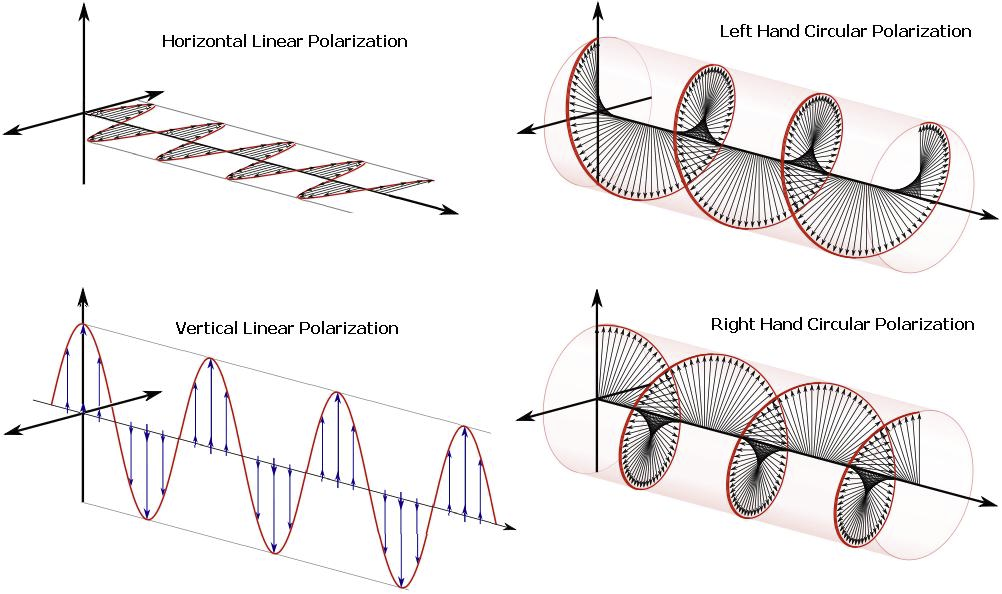
\includegraphics[width=10cm]{gfx/polarizations.png}
 \caption{Distintos tipos de polarizaciones \cite{polarization}}
 \label{fig:hvPolarizations}
\end{figure}

{\textbf{Diagrama de radiación:}} Es la representación gráfica de la densidad de potencia de las ondas radiadas por la antena
en función del ángulo. Típicamente se lo respresenta en un gráfico de tres dimensiones o en diagramas de dos dimensiones de
cortes transversales horizontales y verticales \cite{AntennaWiki}.

\begin{figure}[H]
 \centering
 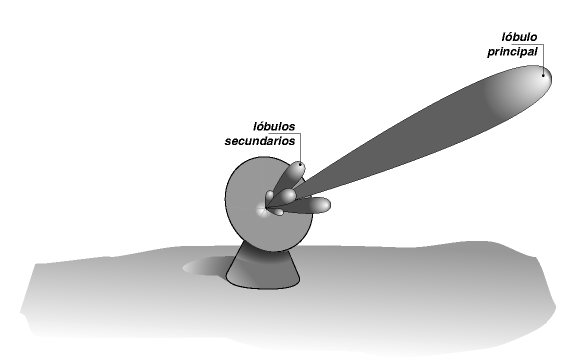
\includegraphics[width=10cm]{gfx/arrayPattern.png}
 \caption{Ejemplo de diagrama de radiación \cite{diagramaRadiacion}.}
\end{figure}

{\textbf{Apuntamiento del haz:}} Es cambiar la dirección del lóbulo principal de un diagrama de radiación \cite{BeamSteering}.

{\textbf{Huella:}} Es el área terrestre visible para el satélite \cite{Footprint}. 

{\textbf{VNA:}} Un VNA es un instrumento que mide los parámetros eléctricos de una red. Hoy, dichos analizadores miden los 
parámetros S porque las reflexiones y transmisiones de redes eléctricas son fácilmente medibles en alta frecuencia. Normalmente
caracterizan redes de dos puertos \cite{NetworkAnalyzer}.

{\textbf{Directividad:}} Es una figura de mérito de una antena. Es el cociente entre la densidad de pontencia radiada en la
dirección de máxima emisión y la densidad de potencia radiada utilizando un radiador isotrópico (el cual emite uniformemente
en toda dirección) \cite{DirectivityWiki}.

{\textbf{SWR o ROE:}} Es una medida de adaptación entre la carga y la impedancia característica de una línea de transmisión. Las
desadaptaciones de impedancias resultan en ondas estacionarias a lo largo de dicha línea de transmisión. El SWR está
efinido como la relación entre la amplitud de la onda reflejada y la amplitud de la onda incidente \cite{swrWiki}.

{\textbf{Adaptación de impedancias:}} La máxima transferencia de potencia requiere que la impedancia de un sistema de
antena esté adaptada al complejo conjugado de la impedancia del transmisor o receptor. En el caso de un transmisor,
la impedancia adaptada deseada no necesariamente corresponde a la impedancia de salida dinámica del transmisor analizado
como una impedancia sino al valor de diseño (típicamente de $50 \Omega$) requerido para una operación eficiente
y segura del circuito de transmisión. Normalmente, la impedancia deseada es resistiva pero un transmisor (y algunos receptores)
pueden tener ajustes adicionales para cancelar una cierta cantidad de reactancia en orden de obtener dicha adaptación. Cuando
una linea de transmisión es utilizada entre la antena y el transmisor (o receptor) uno generalmente desearía un sistema de antena
con una impedancia resistiva cercana a la impedancia característica de dicha línea de transmisión, para minimizar el SWR
e incrementar la transmisión \cite{AntennaWiki}.

{\textbf{Conjunto de Antena con fase variable (en inglés: Phased Array):}} es un conjunto de antenas en que las fases relativas
de las señales con que se alimenta cada antena se varían intencionadamente con objeto de alterar el diagrama de radiación del
conjunto. Lo normal es reforzar la radiación en una dirección concreta y suprimirla en direcciones indeseadas. Si todos los
elementos del conjunto están contenidos en el mismo plano y la señal con que se alimentan es de la misma fase,
entonces se estará reforzando la dirección perpendicular a ese plano. Si se altera la fase relativa de las señales se podrá
\enquote*{mover} el haz (en realidad lo que se está haciendo es cambiar la dirección en la cual las interferencias son
constructivas). Se consigue de este modo hacer barridos sin necesidad de movimiento físico, con la ventaja añadida de que
se pueden barrer ángulos del orden de miles de grados por segundo. Esto permite utilizar la antena para compaginar
simultáneamente funciones de detección y de seguimiento muchos blancos individuales, asi como para obtener imágenes de
apertura sintética. Su uso se va extendiendo debido a la confiabilidad derivada del hecho de que no tienen partes móviles.
Casi todos los radares militares modernos se basan en phased arrays, relegando los sistemas basados en antenas rotatorias a
aplicaciones donde el costo es un factor determinante (tráfico aéreo, meteorología, etc) Su uso está también extendido en
aeronaves militares debido a su capacidad de seguir múltiples objetivos. El primer avión en usar uno fue el B-1B Lancer, y
el primer caza, el MiG-31 ruso.\\

{\textbf{Calibración:}} Operación que, bajo determinadas condiciones, en un primer paso, establece una relación entre
valores cuantitativos con incertidumbres de medición provistas por estándares de medición e indicaciones correspondientes
con incertidumbres asociadas (del instrumento calibrado o estándar secundario) y, en un segundo paso, usa
esta información para establecer una relación para obtener un resultado de una medición desde una indicación \cite{CalDef}.

{\textbf{Calibración interna:}} Las mediciones obtenidas utilizando este sistema son útiles solamente al utilizarlas en
conjuto a los resultados de los test realizados en tierra, los cuales definen la relación entre lo observado y la
performance de los párametros del sistema. Ejemplos de satélites para los cuales se utilizó calibración interna son el
E-ERS-1 y el SIR-C.

Los tests realizados en tierra para dichos sistemas complejos son sobre la electrónica de RF, la electrónica digital y la
antena sobre temperatura; para los cuales es preferible realizarlos, cuando sea posible, en un ambiente al vacío. Los
parámetros clave del sistema, como: potencia transmitida, pérdidas de transmisión o recepción, ganancia de recepción,
ganancia y diagrama de radiación de la antena, linealidad de la electrónica digital/RF, rango dinámico, y fase/amplitud vs
estabilidad de la frecuencia son medidos en función de la temperatura para cada seteo de ganancia del radar y PRF (Pulse
Repetition Frequency). Los elementos de calibración, como medidores de temperatura, de corriente y de potencia, podrán
permitir la determinación dela modela en RF. la performance del sistema en función de la variación de dichos parámetros.

Esta técnica asume que la variación en la performance del sistema puede ser modelada en función de los parámetros observables.
También, se asume que los componentes de calibración están correctamente calibrados y son estables en el paso del tiempo.
Además de estos tests, en la mayoría de los sistemas de radar se realizan mediciones de componentes de RF utilizando lazos de
calibración \cite{Curlander1991}.

{\textbf{Caracterización:}} significa medir (el desempeño de) los parámetros de la antena con el objeto de describir en
forma comprensible su comportamiento \cite{Mittermayer2007}.

{\textbf{Caracterización del sistema:}} adicionalmente incluye la determinación de las curvas de características basadas
en los modelos y en las mediciones indirectas de los parámetros, en el caso en que los parámetros no pueden ser medidos
en forma directa \cite{Mittermayer2007}.

{\textbf{Calibración:}} significa el ajuste de la representación de los parámetros físicos en los productos que arroje la
antena de manera que los mismos puedan ser medidos dentro la especificación \cite{Mittermayer2007}.

{\textbf{Verificación:}} significa mostrar mediante mediciones apropiadas que un sistema o subsistema trabaja dentro de su
especificación (o conjunto de especificaciones) o que un producto cumple con su especificación \cite{Mittermayer2007}.

\section{Contexto} \label{sc:context}

Una antena es un transductor que transforma la energía eléctrica conducida en energía electromagnética radiada cuando
trabaja como transmisora, o viceversa cuando actúa como receptora.

Hay una amplia variedad de antenas en la actualidad, se realiza una agrupación simplificada en la tabla \ref{tab:type_antennas}.

\begin{table}[H]
  \footnotesize
  \centering
  \begin{tabular}{|c|p{9cm}|}
	\hline
	\textbf{Tipo Antena} & \textbf{Características} \\\hline
	Isotrópica & Es una antena hipotética, la cual radía la misma potencia en todas las direcciones.\\\hline
	Monopolo & Es un único módulo radiante, generalmente un simple cilindro de metal conectado en una punta a un plano de
	tierra y en la otra a la línea de alimentación. Usos: Radio AM/FM, walkie talkie, etc. \\\hline
	Dipolo & Es el tipo de antena más comunmente utilizada, consiste en dos RMs simétricos, los cuales son cilindros
	metálicos o cables. Usos: antena de canales de tv VHF, antena de televisión analógica, etc. \\\hline
	Conjunto & Consiste en múltiples antenas trabajando como una única antena. Usos: Transmisión de canales de tv en VHF,
	detección de misiles, comunicaciones satelitales, etc.\\\hline
	Lazo & Consiste en una o múltiples vueltas de cable. Trabajan con campos magnéticos en vez de eléctricos. Usos: receptora
	de canales UHF de tv, receptoras de radio de Amplitud Modulada, etc.\\\hline
	Apertura & Son el principal tipo de antenas direccionales utilizadas en frecuencias microondas. Consisten en una antena
	del tipo dipolo o Lazo junto a una estructura que guía las ondas en una dirección determinada. Usos: Comunicaciones
	satelitales, comunicaciones marinas, etc.\\\hline
  \end{tabular}
  \caption{Cacacterísticas de cada grupo principal de antenas}
  \label{tab:type_antennas}
\end{table}

La presente tesis se enfoca en el tipo \enquote*{conjunto de antena de fase controlada de manera electrónica}, en inglés
\enquote*{phase array electronically controlled antenna}. Este tipo de antenas son ampliamente utilizadas de manera masiva
en aplicaciones donde es necesario realizar apuntamientos en diferentes direcciones con altas velocidades. Por ejemplo,
comunicaciones móviles \cite{Chen2012}, aéreas \cite{MHong1989} y espaciales \cite{Shimada1995}\cite{Makhoul2012}. En el capítulo
\ref{ch:phasedArray} se explica el principio de funcionamiento básico de dicho tipo de antena.

Para generar diversos productos, por ejemplo imágenes satelitales en radares SAR \cite{Freeman1992}, es necesario que la
antena se encuentre correctamente calibrada \cite{Luscombe1990}\cite{Seifert1996}\cite{Dall1994}. Esto implica, que las
tolerancias de fase y amplitud se mantengan en el tiempo y/o sus valores sean bien conocidas para cada elemento del conjunto.

Un método de calibración en tierra para estas antenas es la de utilización de fuentes externas de campo lejano o cercano
\cite{Agrawal2003}. Sin embargo, en aplicaciones aéreas o espaciales, la utilización de dichas fuentes es impráctica o
difícil de implementar \cite{Aumann1989}. Para estos casos se utilizan esquemas de calibración externa e interna.

Hay dos grupos principales de calibración externa a saber,
\begin{itemize}
	\item Calibración utilizando blancos puntuales: Los blancos puntuales son dispositivos construidos por el hombre, generalmente
		corner reflectors, transponders, generadores de tono o receptores. La característica de estos dispositivos es que no
		solo son muy chicos con respecto a la mínima área de observación de una antena y que el eco de la señal de dichos
		dispositivos posee mucha más intensidad que dicha área, sino que el reflejo es bien conocido. Por lo tanto, con su uso
		se puede deducir la potencia transmitida.
	\item Calibración utilizando blancos distribuidos: Se refiere a la utilización de blancos naturales de largas áreas con
		propiedades de dispersión homogéneas. Se utiliza la suposición que dichas propiedades son estables o que su variación es
		bien conocida.
\end{itemize}

El mayor problema de dichos esquemas de calibración es que el tiempo de revisita a dichos lugares de calibración en tierra es muy
grande y solo se puede calibrar la ganancia absoluta del conjunto de antena en su totalidad. Para disminuir el tiempo entre
calibraciones y para poder calibrar cada elemento del conjunto de forma individual surge diversos esquemas de calibración
interna.

El primer método a mencionar es el llamado método REV, el cual calibra de a un módulo radiante a la vez utilizando una
antena externa al panel como receptora. En el proceso de calibración se transmite de a un módulo radiante a la vez
y se va variando su fase hasta obtener la máxima potencia recibida. Repitiéndose el proceso para todos los elementos.

Otro método es el convencional (descripto en el capítulo \ref{ch:classicalCalibration}), el cual implementa lazos internos
para calibrar los caminos de transmisión y recepción de la antena de forma independiente \cite{Makhoul2012}
\cite{Luscombe1990}\cite{Seifert1996}\cite{Dall1994}\cite{Freeman1995}\cite{Bibby2003}\cite{Bast2003}\cite{Stove2004}
\cite{Srivastava1996}\cite{Wang2010}. Para ello, la señal de calibración recibida se la compara con la potencia transmitida,
obteniendo así, que dicha diferencia se corresponde con el desfasaje de potencia y fase de cada camino de transmisión/
recepción. Luego, se opta por caracterizar todos aquellos componentes que no pertenecen a ningún lazo de calibración
\cite{Freeman1995}. Este método presenta algunos inconvenientes. Por dar un par de ejmplos se puede mencionar que los recursos
necesarios (tiempo, personal) durante la campaña de ensayos previa al lanzamiento impactan en todo el desarrollo de actividades,
o las consecuencias que puede traer el hecho que la caracterización no sea válida porque un determinado componente
envejece con el paso del tiempo.

En este contexto, se investiga y propone un método que permita reducir costos asociados a la calibración y por ende a los
proyectos:

\begin{enumerate}
    \item Evitando la necesidad de realizar caracterizaciones previas del conjunto de antena.
    \item Permitiendo conocer en tiempo real, y para el estado real de la antena, los valores reales de fase y amplitud en
		vuelo que transmite la antena, independientemente de su estado de envejecimiento.
\end{enumerate}

En este sentido se investiga y aprovecha el concepto acoplamiento mutuo inherente entre los módulos radiantes de la antena
\cite{Aumann1989}, pero de manera complementaria al enfoque tradicional. Este método calibra tanto los caminos de transmisión
como recepción a la vez, para ello, se transmite en una polarización y se recibe en otra de a un módulo radiante a la vez.
Una ventaja que tiene frente a los otros métodos realizados es que no solo calibra la antena en su totalidad, sino también
sirve para determinar si hay módulos radiantes en mal funcionamiento o directamente inhabilitados.

\section{Motivación} \label{sc:motivation}

Para poder hacer un uso adecuado del PA es necesario conocer la fase y atenuación de cada uno de los elementos del mismo, tanto
cuando transmiten como cuando recibe. Sn embargo, si bien uno controla la fase y atenuación de cada elemento, la RFDN no permite
necesariamente asegurar que la fase y atenuación con que sale la señal sea realmente la deseada. Hay fenomenos de dispersion en
la RFDN debidos a la temperatura que hacen que la fase deseada y la requerida sean diferentes \cite{Keizer2011}.

El método de calibración tradicional, por lazos de calibración internos, permite calibrar un conjunto de antena, aunque
adolece de algunos defectos entre los cuales se incluyen:

\begin{enumerate}
    \item Un mal funcionamiento o directamente la inhabilitación de un elemento radiante, el cual está fuera del lazo de
		calibración interno, no es detectado por la calibración interna.
    \item Existen elementos que quedan fuera del lazo de calibración interna. Como por ejemplo los circuladores. Esto lleva a
		la necesidad de realizar caracterizaciones en tierra, lo cual implica un consumo de recursos de proyecto importantes,
		además de tener que confiar que dicha caracterización será válida (o sea que no habrá envejecimiento de los mismo)
		durante toda la vida útil de la antena.
    \item Cada lazo de calibración no se interrelaciona con el resto haciendo que no se pueda disminuir el error de medición por
		multiplicidad de caminos.
\end{enumerate}

El conocimiento de dichas limitaciones llevan a investigar opciones superadoras, que den lugar a un método de calibración que 
permita ser complementario al tradicional. 
\begin{enumerate}
	\item Evitando la necesidad de realizar costosas caracterizaciones en tierra
	\item Previendo que los componentes en vuelo puedan envejecer y por ende modificar sus características.
	\item Permitiendo detectar fallas en elementos que en la calibración interna tradicional están fuera del lazo de calibración.
	\item Disminuyendo la incertidumbre en la determinación de la fase y amplitud de salida.
\end{enumerate}

El método proupesto en esta tesis, denominado de \enquote*{diseño y calibración de una antena polarimétrica por 
acoplamientos mutuos}, toma la idea de mediciones por acoplamiento mutuo \cite{Agrawal2003}\cite{Shipley2000} \cite{Aumann1989}
\cite{Chen2012} para integrarla de manera complementaria al método tradicional sin necesidad de agregar hardware adicional. 
Además, se establecen los requerimientos electrónicos para poder implementarla. Para poder comparar el coportamiento y 
eficiencia de ambos métodos, se realiza un modelo de antena polarimétrica.

\section{Objetivo de la Tesis} \label{sc:objective}

La presente tesis tiene varios objetivos:

\begin{enumerate}
    \item Presentar conceptualmente el método tradicional de calibración interna de una antena polarimétrica. Con sus 
		virtudes y defectos. Mencionar algunas misiones de ejemplo en las cuales el mismo se ha utilizado.
    \item Investigar, desarrollar y presentar conceptualmente un método alternativo de calibración interna que introduzca
		mejoras al método tradicional sin necesidad de introducir hardware adicional y con la premisa fundamental de
		reducir los costos asociados a las caracterizaciones que el método tradicional incluye. Introducir los
		requerimientos necesarios para poder implementarlo.
    \item Investigar e implementar el modelo de antena polarimétrico que será utilizado para poder comparar el 
		método tradicional y el alternativo. Dicho modelo debe representar el comportamiento en RF básico de las señales al 
		propagarse por el sistema.
    \item Implementar los sistemas de calibración tradicional y alternativo que actúen sobre el modelo de antena. 
    \item Sacar conclusiones respecto a los pros y contras del método propuesto, en particular en referencia al método
		tradicional, por medio de algunos parámetros objetivos como ser tiempo de calibración, caracterizaciones necesarias,
		incertidumbre de medición, entre otros.
\end{enumerate}


\section{Especificaciones del problema} \label{sc:specifications}

Para poder aplicar e implementar el método de acoplamientos mútuos se deben cumplir las siguinetes hipótesis de base, que a su
vez son consideradas las especificaciones del problema.

\begin{enumerate}
    \item Modularización de los componentes de la antena: La antena debe estar compuesta por defasadores, atenuadores, cables,
		divisores de potencia y elementos radiantes.

	\item Modelización de los componentes en RF: Los componentes de la antena deben caracterizarse utilizando parámetros de alta
		frecuencia.

    \item Sistemas LTI: La aplicación deberá reproducir el comportamiento del sistema, el cual será LTI (lineal e invariante
		en el tiempo).

	\item Adaptación de impedancias: Todos los componentes se encuentran perfectamente adaptados.

    \item Variabilidad para determinados componentes: Se deben poder utilizar distintos divisores/combinadores de potencia.
		La diferencia entre ellos es la cantidad de puertos de salida.

    \item Dimensión de antena: Se debe poder configurar la cantidad de elementos radiantes por columna y fila de la antena.
    \item Distancia entre elementos radiantes: Se debe poder configurar la distancia entre elementos radiantes.
    \item Configuración individual de componentes: Se debe poder configurar los atributos que afecten la modelización de cada
		componente de la antena. Largo, atenuación y defasaje por metro de cables.

    \item Modelizaciones dispersiones: Se debe poder configurar la dispersión en el comportamiento de cada componente de la
		antena de forma independiente.

    \item Introducción de elementos de control en el lazo de calibración: Se deben poder configurar los atenuadores y
		defasadores a la hora de realizar la calibración.

    \item Calibración clásica: La aplicación debe poder calibrar una antena polarimétrica con el método de calibración convencional.

    \item Calibración alternativa: La aplicación debe poder calibrar una antena polarimétrica con el método de calibración alternativo.

    \item Calibración ganancia: La aplicación debe poder calibrar la ganancia de transmisión y recepción.

    \item Calibración fase: La aplicación debe poder calibrar la fase de transmisión y recepción.

    \item Cal. pol. horizontal: La aplicación debe poder calibrar en la polarización horizontal.
    \item Cal. pol. vertical: La aplicación debe poder calibrar en la polarización vertical.
    \item Cal. Tx: La aplicación debe poder calibrar en transmisión.
    \item Cal Rx: La aplicación debe poder calibrar en recepción.

    \item Calibración independiente del estado inicial: Se debe poder alcanzar el estado de calibración deseado partiendo
		cualquier estado inicial en los defasadores y atenuadores.

    \item Transmisión vs recepción por polarizaciones cruzadas: Para calibrar se debe transmitir y recibir en polarizaciones
		diferentes.

    \item Planitud de antena: La antena tiene que ser perfectamente plana. No deben haber imperfecciones.

    \item Frecuencia de RF: Se debe poder configurar la frecuencia de trabajo.

    \item Dispersión señal de calibración entre pulsos: Se debe poder configurar los parámetros de dispersión (desvío estándar) para
		la ganancia y fase de la chirp utilizada entre pulsos.

    \item Dispersión chirp réplica: Se debe poder configurar los parámetros de dispersión (desvío estándar) para la
		ganancia y fase de la chirp réplica utilizada a la hora de realizar la calibración convencional.

    \item Dispersión walsh: Se debe poder configurar los parámetros de dispersión (desvío estándar) para la fase de la
		codificación utilizada a la hora de realizar la calibración convencional.

    \item Simulación falla componente: Se debe poder simular, configurar la destrucción total de los TRMs o RMs de la antena.
\end{enumerate}


\section{Metodología de la tesis} \label{sc:methodology}

\todo{comence a cambiar por aca}
En la presente tesis se investiga sobre las posibles modulaciones de la señal transmitida y las distintas topoligías del radar
de onda contínua modulada en frecuencia (FMCW).

Posteriormente, en función de lo investigado previamente, la tarea a determinar en el área de investigación y las 
características de cada componente, se determina la topología del radar en su totalida.

Luego, se construye un modelo de ingeniería del radar para determinar cuan preciso puede llegar a ser y deterimnar las posibles
complicaciones. Para validar se desarrolla un modelo del radar, donde se puede simular una adquisición completa. 

Finalmente se prueban, analizan y documentan los resultados obtenidos de distintas mediciones con el radar, haciendo mención de
posibles mejoras y cambios a realizar tanto en el programa que procesa la señal recibida como de la topología del radar.


\section{Contribución} \label{sc:contribution}

Como contribución se desarrolla un simulador que modela el radar, la señal transmitida, recibida y el blanco iluminado. 
Cumpliendo así con todos los requerimientos del problema previamente mencionados, logrando así, que sea representativo en RF.
A su vez, se construye un modelo de ingeniería del radar para tomar mediciones y determinar la matriz de parámetros S de los
blancos iluminados. Se puede utilizar dicho modelo de ingeniería para futuros proyectos de mayor envergadura. 


\section{Estructura de la Tesis} \label{sc:structure}

Los siguientes capítulos se organizan de la siguiente manera:

\begin{enumerate}
	\item Capítulo 2: Se presenta y detalla una antena polarimétrica, haciendo hincapié en el diagrama de radiación y como
    se realiza su modelización en RF.
	\item Capítulo 3: Se presenta y detalla el método de calibración clásica plantenado sus ventajas y desventajas.
	\item Capítulo 4: Se presenta y detalla el método de calibración por acoplamientos mutuos planteando sus ventajas y
		desventajas.
	\item Capítulo 5: Se detalla la modelización y estructura del modelo de la antena implementado para realizar los ensayos.
	\item Capítulo 6: Se presentan los ensayos realizados sobre el modelo de antena utilizando distintos factores de errores y
		comparando los resultados obtenidos por ambos calibradores.
	\item Capítulo 7: Se presentan los resultados obtenidos, conclusiones y posibles trabajos futuros a realizar.
	\item Apéndices
\end{enumerate}


%% Chapter 2

\chapter{Introducción a las antenas polarimétricas} % Chapter title
\label{ch:phasedArray}
\lhead{\emph{Introducción a las antenas polarimétricas}}
%----------------------------------------------------------------------------------------

\section{Antenas polarimétricas}

Una antena polarimétrica es una antena que es utilizada, por ejemplo, en radares y satélites. Las mismas pueden ser activas 
o pasivas, esto es, para el primer caso, que el sistema emita su propia energía, para luego medir el eco de la misma (por 
ejemplo el radar SIR-C \cite{Curlander1991}). Para el segundo caso, el radar no emite ninguna señal, simplemente recibe el eco 
de algún otro sistema emisor/receptor.

\begin{figure}[H]
 \centering
 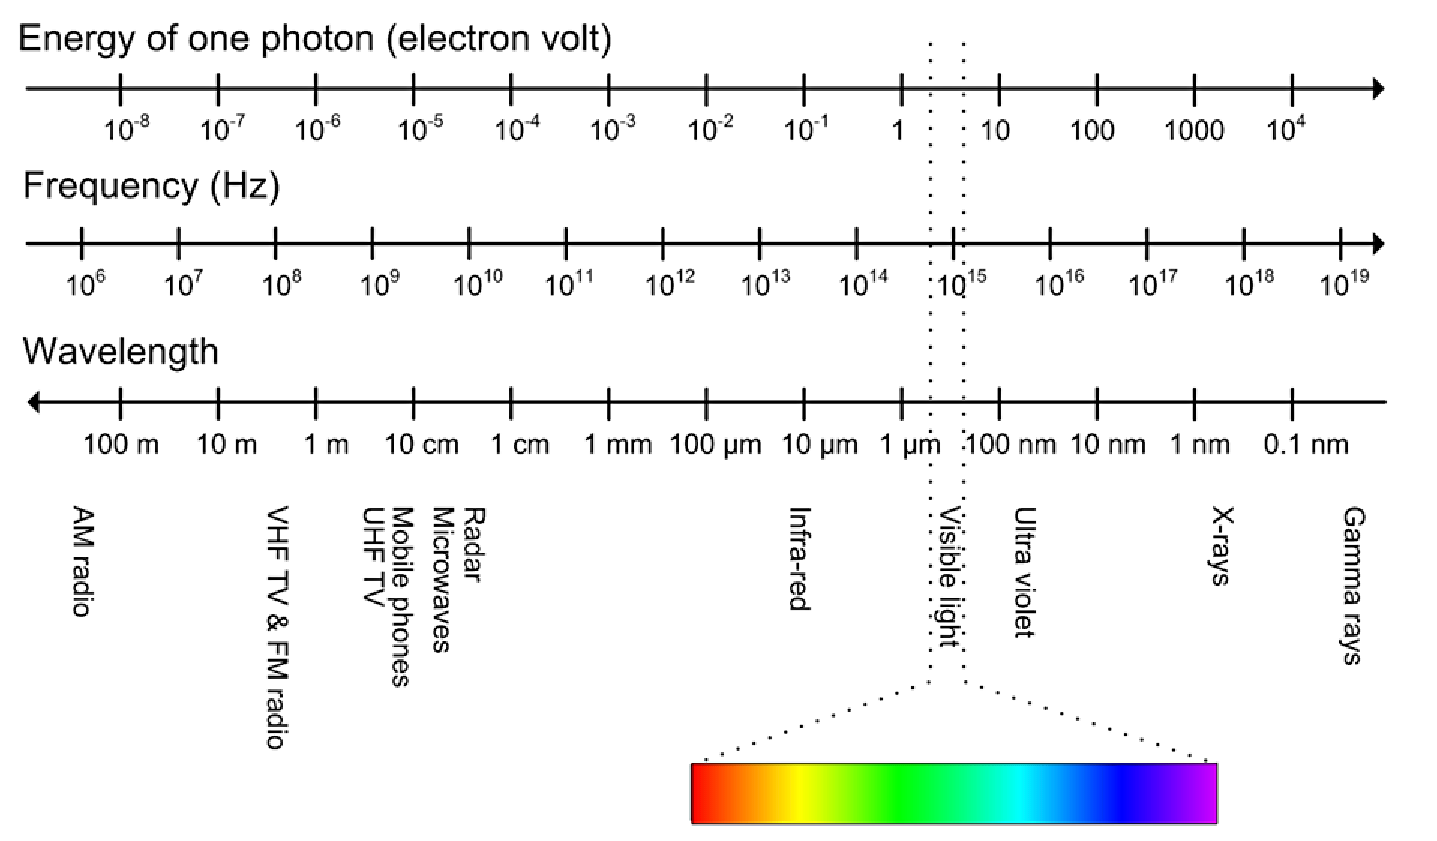
\includegraphics[width=10cm]{gfx/electromagneticSpectrum.png}
 \caption{Espectro Electromagnético \cite{electromagneticField}}
 \label{fig:spectrum}
\end{figure}

Dado que la frecuencia de trabajo mayormente utilizada en este tipo de antenas comprende la región microondas del espectro
electromagnético, el cual comprende desde los 300 MHz hasta los 300 GHz (ver figura \ref{fig:spectrum}), y dado que en dicho rango la 
opacidad de la atmósfera es casi nula (ver figura \ref{fig:atmosphere}), puede decirse, en terminos generales, que dichas 
antenas poseen la capacidad de trabajar independientemente de las condiciones atmosféricas. En otras palabras, la señal casi no es 
atenuada por la atmósfera, tampoco es interferida ni por las lluvias ni por las nubes. Por ejemplo, si se usa como parte de un 
radar de apertura sintetica, luego de un post procesamiento de la señal recibida, es posible obtener información sobre la 
textura del terreno y sobre los sustratos inferiores de las coberturas boscosas. Dependiendo de que longitud de onda del rango de
trabajo, se tiene de 3 cm a 30 cm de penetración.

\begin{figure}[H]
 \centering
 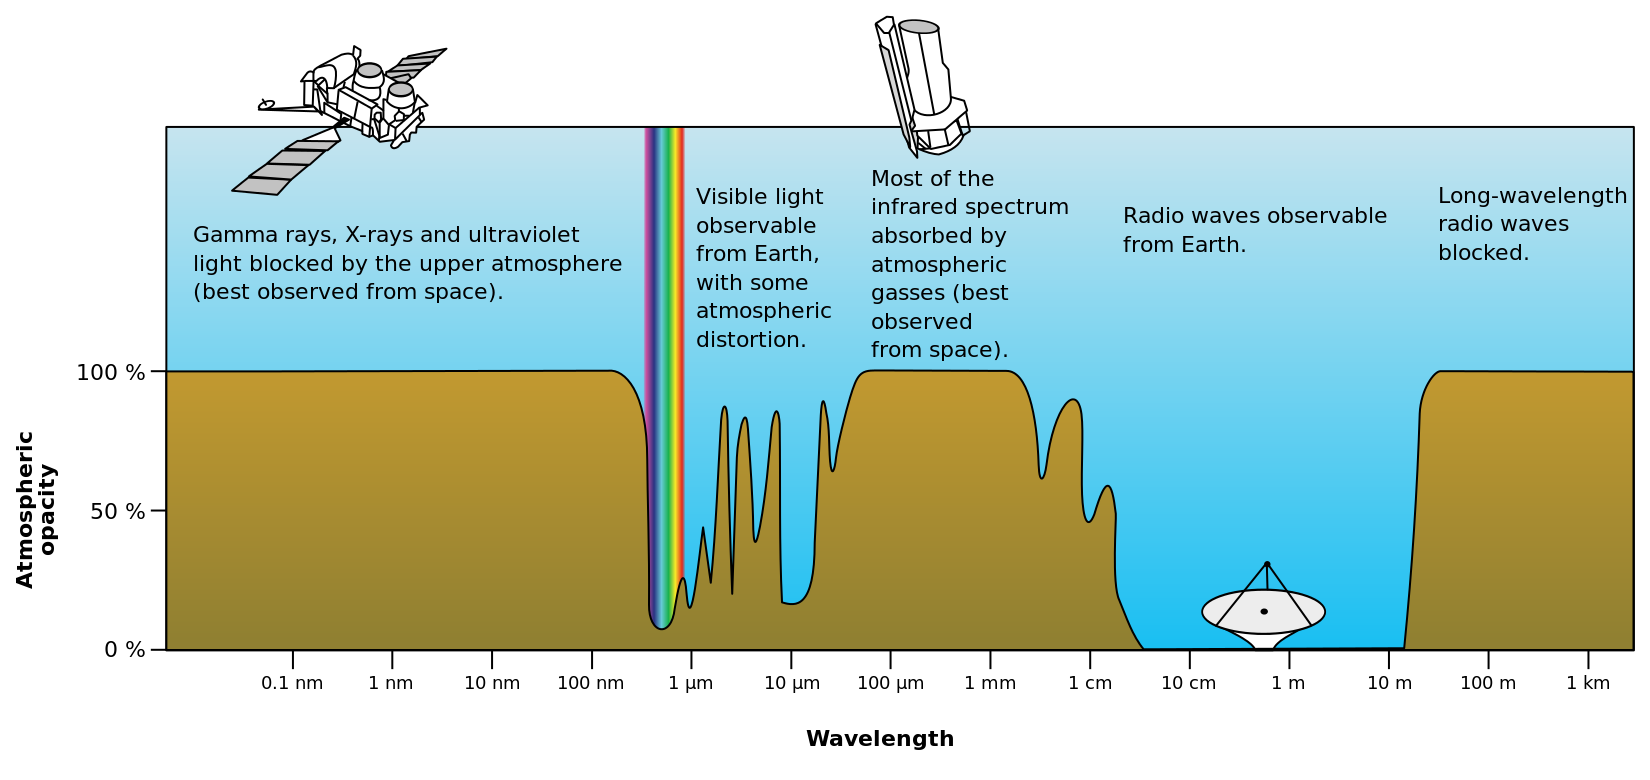
\includegraphics[width=10cm]{gfx/AtmosphericOpacity.png}
 \caption{Opacidad atmosférica vs longitud de onda \cite{electromagneticOpacity}}
 \label{fig:atmosphere}
\end{figure}

Por convención, el eje de referencia paralelo a la dirección del recorrido del satélite es llamado azimuth y la
dirección del eje perpendicular, rango. El nadir es el punto más cercano de la tierra al satélite; en otras palabras,
es el punto en la superficie terrestre que es cortado por una recta perpendicular que también corta al satélite.

La antena nunca apunta diréctamente hacia abajo porque, de esta forma, se perdería mucha información en rango. Al apuntar
en diagonal, y gracias a que el blanco no es puntual, el eco de la señal de la zona iluminada más cercana al nadir llega
antes al satélite que la más alejada, logrando así, tomar muestras de distintos lugares espaciados en rango (ver figura
\ref{fig:antena_ilumination}).

\begin{figure}[H]
 \centering
 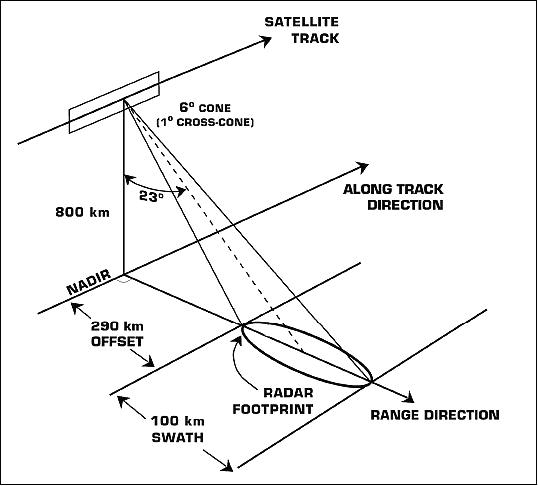
\includegraphics[width=7cm]{gfx/satellite.png}
 \caption{Footprint del satélite \cite{FootprintSatellite}.}
 \label{fig:antena_ilumination}
\end{figure}

El tamaño de la zona iluminada se llama huella. Dicho tamaño depende tanto de las dimensiones de la antena como de la
órbita del satélite o de la altura del avion en que está colocada dicha antena. Como se observa en la imagen
\ref{fig:footprint}, mientras más larga es la antena, más angosto es el footprint, logrando así mejorar la resolución
espacial.

\begin{figure}[H]
 \centering
 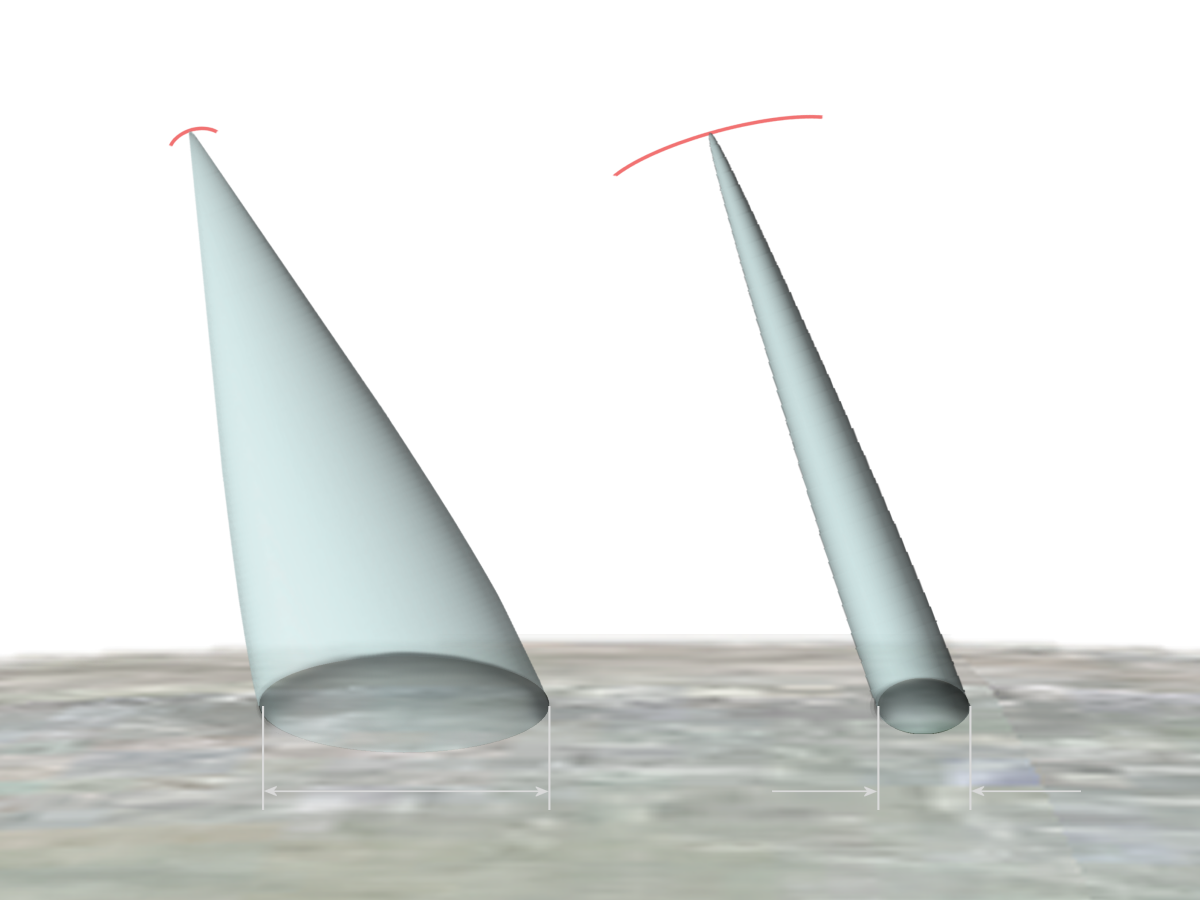
\includegraphics[width=7cm]{gfx/footprint.png}
 \caption{El footprint depende del largo de la antena \cite{FootprintAntenna}.}
 \label{fig:footprint}
\end{figure}

\subsection{Composición de una antena}

Un conjunto de antena polarimétrica consta de una colección de $N$ elementos radiantes. Se asume que dichos elementos poseen el
mismos diagrama de radiación y que están orientados en el mismo sentido y dirección en un ambiente tridimensional. No es
necesario que estén espaciados regularmente ni que emitan los mismos valores de potencia y fase, pero si se asume
que todos están alimentados con la misma frecuencia de trabajo. En la figura \ref{fig:phasedArrayAntenna} se pueden observar
dos tipos de distribuciones comunmente utilizadas.

\begin{figure}[H]
	\centering
 	\subfloat[]{
		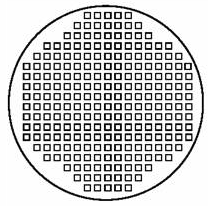
\includegraphics[width=4cm]{gfx/phasedArrayAntenna.png}}
	\subfloat[]{
		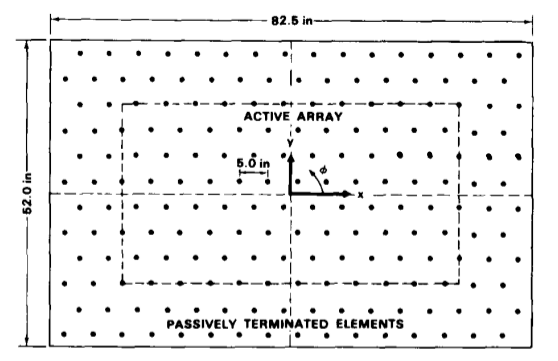
\includegraphics[width=6cm]{gfx/frontAntenna.png}}
		\caption{Conjuntos de antena: (a) Circular \cite{AntennaFront}. (b) Rectangular \cite{Aumann1989}.}
	\label{fig:phasedArrayAntenna}
\end{figure}

Este tipo de antenas está compuesto por dos bloques principales a saberi: la red de distribución (o RFDN) y los elementos 
radiantes (ver figura \ref{fig:compositionAntenna}).

\begin{figure}[H]
 \centering
 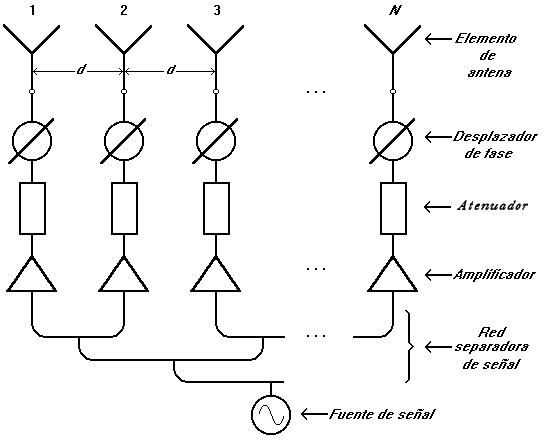
\includegraphics[width=10cm]{gfx/CompositionAntenna.png}
 \caption{Composición de un conjunto de antena}
 \label{fig:compositionAntenna}
\end{figure}

El generador puede emitir distitnos tipos de modulaciones. Ej, cuadrada, chirp, senoidal, triangular, etc. Las ventajas y
desventajas de cada una se lista en el cuadro \ref{tab:modulations}

\begin{table}[H]
  \footnotesize
  \centering
  \begin{tabular}{|c|p{9cm}|}
	\hline
	\textbf{Modulación} & \textbf{Cacarcterísticas} \\
	Cuadrada & Esta modulación es utilizada para mediciones muy precisas a cortas distancias comparando las fases de los dos
	semiciclos de la señal recibida. La desventaja es que los distintos ecos de los distintos blancos no pueden distinguirse.\\\hline
	Chirp & Es la modulación mayormente utilizada, se obtienen mediciones con las mayores distancias posibles.\\\hline
	Triangular & Con esta modulación se logra distinguir fácilmente la velocidad de la posición del blanco. \\\hline
	Escalonada & Es utilizada para mediciones de interferometría y para expandir el rango de medición sin ambig\"uedades.\\\hline
  \end{tabular}
  \caption{Cacacterísticas de cada modulación de la señal emitida}
  \label{tab:modulations}
\end{table}

La red de distribución, llamada RFDN, es la encargada de transmitir la señal a todos los elementos radiantes de la antena.
Dicha red posee una estructura de árbol, de forma tal, que la longitud de todos los caminos entre las hojas del mismo a
la raíz son iguale (Los nodos son los PSC y las hojas los RMs). Es necesraio que todos los caminos sean iguales para que las
señales transmitidas posean la misma fase y atenuación. Los componentes utilizados para distribuir la señal son los siguientes:

\begin{itemize}
	\item Divisor/Combinador de potencia de RF: este componente es el encargado de dividir la señal transmitida en tantos puertos 
		de salida tenga y la de sumar/combinar las potencias recibidas.
	\item Cable: este componente es el utilizado para unir el resto de los componentes.
	\item Módulo de Transmisión y Recepción: Este componente es el elemento de control de fase y atenuación de la señal emitida y
		recibida por la antena. Para la modelización realizada, se considera que hay uno por cada elemento radiante.
	\item Defasador: Este componente simplemente defasa la señal, hay uno por cada elemento radiante, se lo utiliza
		para poder calibrar la antena tanto en transmisión como en recepción, logrando así, que cada camino de transmisión/
		recepción de las hojas a la raíz defasen lo mismo. A su vez, se lo utiliza para poder direccionar el beam de la señal
		emitida.
	\item Elemento Radiante: Este componente es el emisor de la señal a transmitir y/o el receptor. En este tipo de antenas un
		RM puede cumplir una o ambas funcionalidades.
	\item Circulador: Este componente posee tres puertos y es utilizado para separar los caminos de la señal transmitida (Tx) de 
		la recibida (Rx) cuando un mismo elemento radiante posee las funcionalidades de transmisión y recepción. 
\end{itemize}

Se pueden conectar los elementos radiantes de tal forma que puedan transmitir en dos polarizaciones distintas, H y V (Ver figura
\ref{fig:polarizations}), para esto, se debe duplicar la RFDN. Haciendo uso de ambas polarizaciones se puede caracterizar
los blancos observados, dado que, cada cuerpo responde de forma distinta a cada tipo de polarización.

\begin{figure}[H]
 \centering
 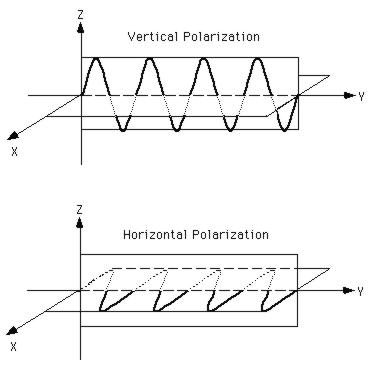
\includegraphics[width=7cm]{gfx/HAndVPolarizations.png}
 \caption{Polarizaciones verticales y horizontales}
 \label{fig:polarizations}
\end{figure}


\subsection{Diagrama de radiación de antena}

Un conjunto de antena puede armarse recursivamente, esto es, que un elemento sea, en si mismo, un conjunto. Un diagrama de antena es
un diagrama de radiación polar que resulta de reemplazar cada elemento por un radiador isotrópico. Si se asume que el diagrama de
radiación de cada elemento es idéntico al del resto, tomando una cierta incertidumbre, el diagrama de radiación total resulta de
la multiplicación de todos los diagramas de todos los elementos. Este resultado no depende de si se consideran los diagramas de
potencia o de amplitud/fase.

\begin{figure}[H]
 \centering
 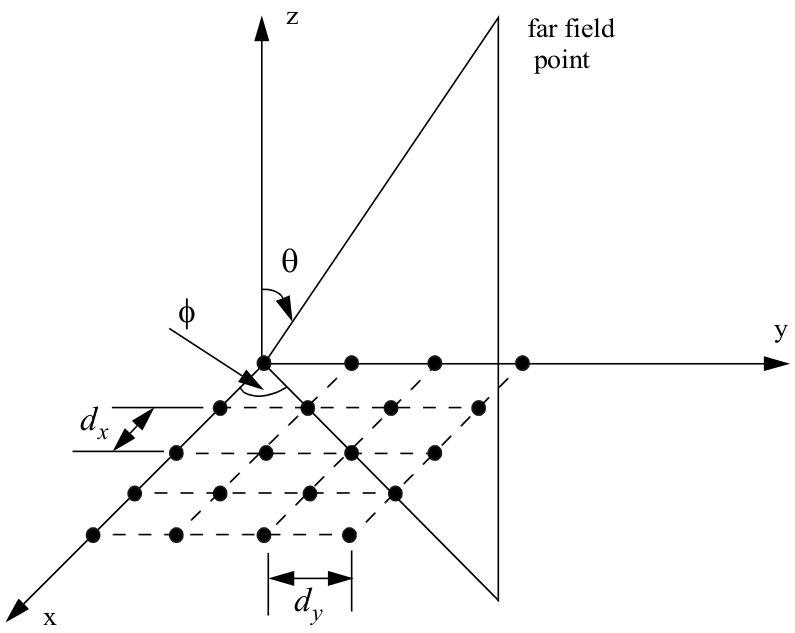
\includegraphics[width=7cm]{gfx/rectangularArrayGeometry.png}
 \caption{Conjunto de geometría rectangular \cite{Mahafza2004}}
 \label{fig:arrayGeometry}
\end{figure}

Considerese un conjunto de antena de $NxM$ elementos, como se muestra en la figura \ref{fig:arrayGeometry}, el diagrama de
radiación de campo lejano se lo calcula de la siguiente forma \cite{Mahafza2004}.

\begin{equation}
	E(\theta, \phi) = \sum_{n=0}^{N-1}\sum_{m=0}^{M-1} I_{n,m} e^{jk(d_xn\sin\phi\cos\theta + d_ym\sin\phi\sin\theta)}
\end{equation}

Donde $\theta$ corresponde al ángulo al eje x, $\phi$ corresponde al ángulo al eje z, $k$ es el número de onda y es igual
a $2\pi/\lambda$, $I_{n,m}$ es la amplitud compleja del elemento $n,m$. La figura \ref{fig:arrayPattern} muestra el diagrama de
radiación en tres dimensiones, donde el eje $Z$ (representado con colores) es la potencia radiada. A su vez, se puede apreciar 
uno de los cortes que se realizan generalmente sobre los mismos (elevacion o azimuth).

\begin{figure}[H]
 \centering
	\subfloat[]{
		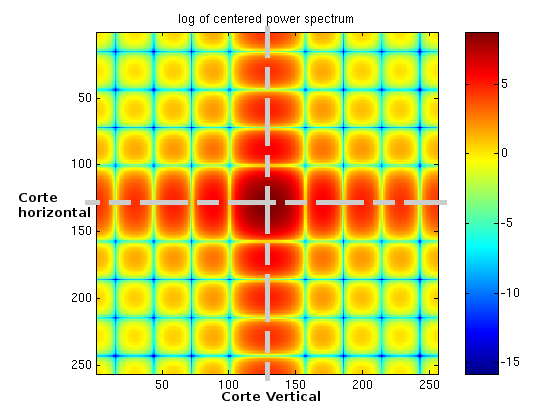
\includegraphics[width=7cm]{gfx/arrayPattern3D.png}}
 	\subfloat[]{
		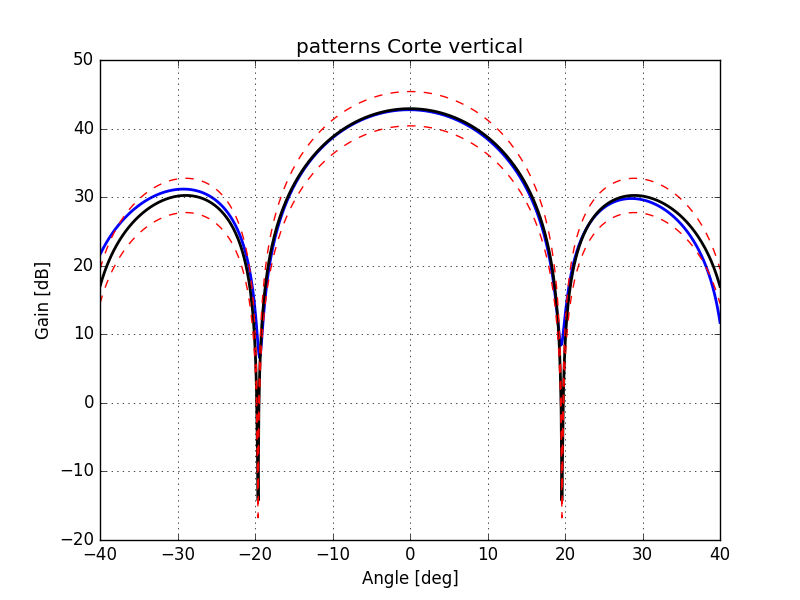
\includegraphics[width=7cm]{gfx/arrayPatternCut.png}}
	\caption{diagramas de radiación de un conjunto de antena (a) diagrama en 3 dimensiones \cite{arrayPattern} (b) corte horizontal}
 \label{fig:arrayPattern}
\end{figure}

Los tres parámetros más importantes del diagrama de radiación son la directividad, el ancho del lóbulo principal y el nivel
de los lóbulos secundarios \cite{Hsiao1985}. Es importante incrementar lo más posible la diferencia de potencia entre los 
lóbulos secundarios y el principal. Para lo cual, si se desea realizar un achicamiento de los lóbulos secundarios sin modificar 
la directividad como el ancho del lóbulo principal, es necesario incrementar el tamaño del conjunto de antena \cite{Hsiao1985}. 
Lamentablemente los errores, incertidumbres y desvíos en el comportamiento del conjunto limitan los niveles que se pueden 
obtener de los lóbulos secundarios \cite{Hsiao1985}.

A continuación se muestran gráficos representando la potencia del campo radiado, asumiendo campo lejano. La potencia decae
con la relación de $1/r$, donde $r$ es la distancia del punto de medición al elemento radiado. Se debe tomar en cuenta también
la fase con que emite el elemento y el retardo de fase que se debe a la distancia recorrida por la señal para llegar a los 
distintos lugares del espacio. Dicho retardo es expresado como $2\pi r/\lambda$, siendo $\lambda$ la longitud de onda de la 
señal emitida por el elemento radiado. Los gráficos \ref{fig:twoArrayPat} y \ref{fig:fourArrayPat} muestran las curvas de 
nivel de diagramas de radiación de pontencia polar, donde los elementos radiantes están distribuidos uniformemente sobre el eje
x (eje horizontal) y emiten en fase.

\begin{figure}[H]
	\centering
	\subfloat[]{
		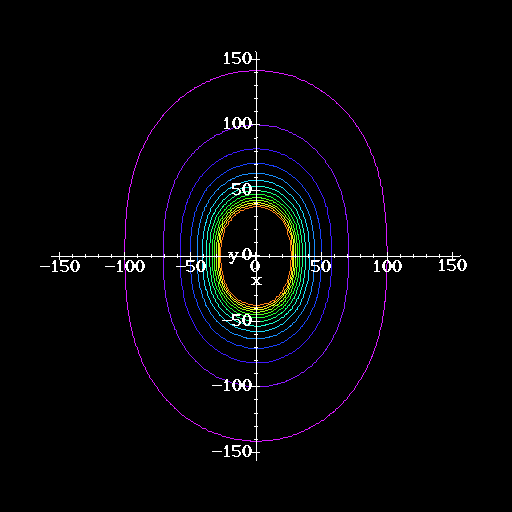
\includegraphics[width=5cm]{gfx/TwoIsoQuartDist.png}}
	\subfloat[]{
		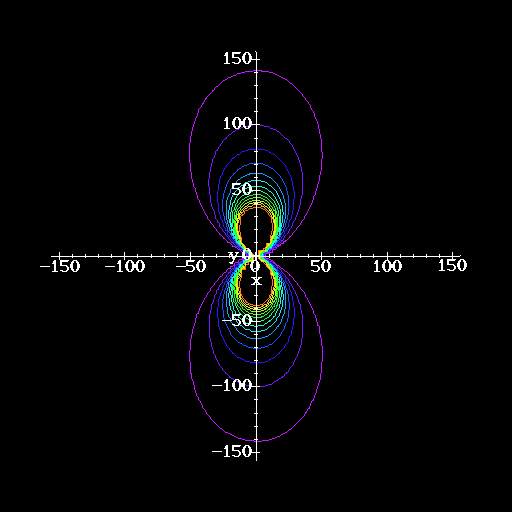
\includegraphics[width=5cm]{gfx/TwoIsoHalfDist.png}}
	\caption{Diagramas de radiación de potencia. Dos RMs con separación de: a) $1/4$ de longitud de onda, b) $1/2$ de longitud de onda}
	\label{fig:twoArrayPat}
\end{figure}

\begin{figure}[H]
	\centering
	\subfloat[]{
		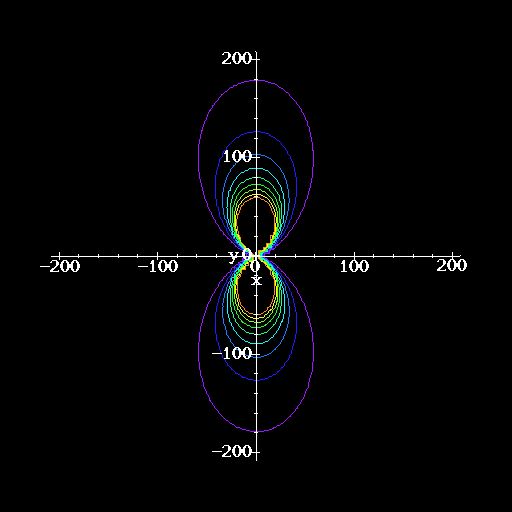
\includegraphics[width=5cm]{gfx/FourIsoQuartDist.png}}
	\subfloat[]{
		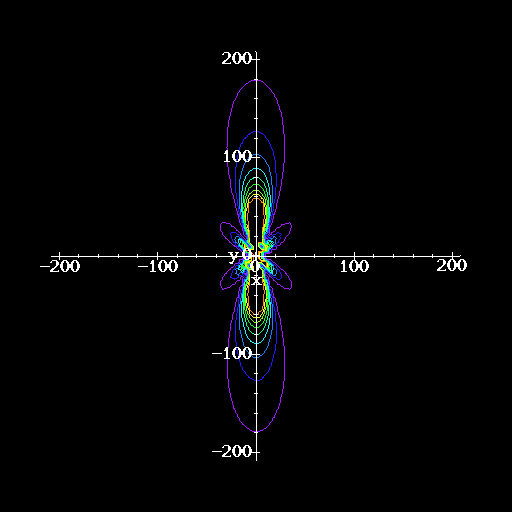
\includegraphics[width=5cm]{gfx/FourIsoHalfDist.png}}
	\caption{Diagramas de radiación de potencia. Cuatro RMs con separación de: a) $1/4$ de longitud de onda, b) $1/2$ de longitud
		de onda}
	\label{fig:fourArrayPat}
\end{figure}

Se puede observar que aumentando la cantidad de elementos radiantes, se logra que el haz principal (lóbulo principal de
potencia) sea más angosto, por lo tanto se obtenga una mayor resolución del cuerpo observado. La figura \ref{fig:directArrayPat} 
muesra que la fase con que emiten los elementos radiados modifica el apuntamiento de la antena.

\begin{figure}[H]
	\centering
	\subfloat[]{
		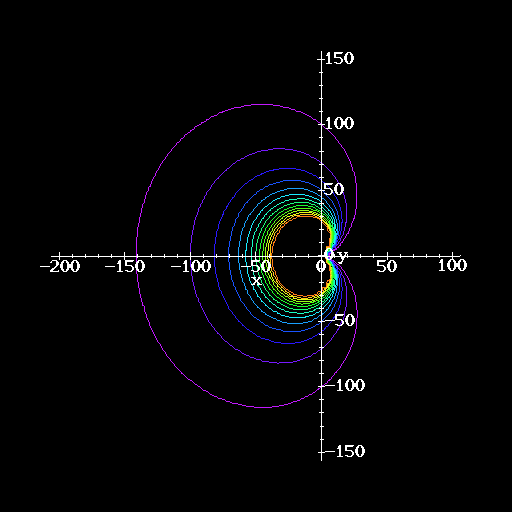
\includegraphics[width=5cm]{gfx/TwoQuarterPhase.png}}
	\subfloat[]{
		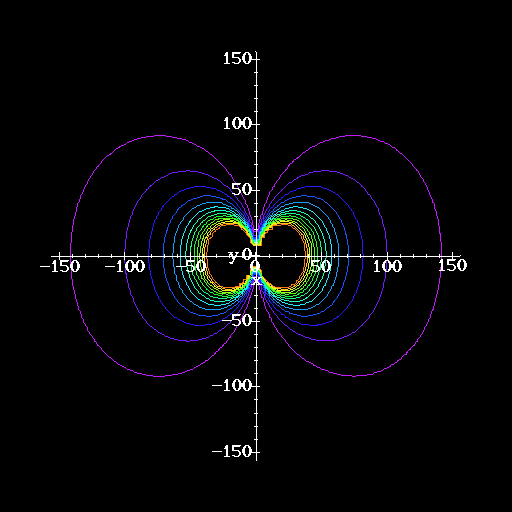
\includegraphics[width=5cm]{gfx/TwoAntiPhase.png}}
	\caption{Diagrama de radiación de potencia. Dos RMs en contrafase y con separación de: a) $1/4$ de longitud de onda. b) $1/2$ 
		de longitud de onda}
	\label{fig:directArrayPat}
\end{figure}


\subsection{Apuntamiento de una antena}\label{ssec:beamSteering}

Para que la suma de todas las señales emitidas con todos los elementos radiantes apunte a un mismo punto, es necesario que
todas las ondas lleguen al objetivo con la misma fase. Es por esto que se debe saber determinar cual es la fase individual que
debe tener cada uno de los elementos radiantes.

Como primer simplificación, se puede asumir que todas las rectas de cada uno de los elementos radiantes al punto lejano son
paralelas entre ellas. A su vez, como el camino recorrido desde cada elemento radiante al punto lejano es diferente, es
necesario calcular dicha diferencia para luego relacionarla con la fase. De esta forma, se puede retrasar la fase emitida de
los elementos más alejados al punto para que todas las señales lleguen en fase, logrando así, una onda plana.

La figura \ref{fig:beamSteering} muestra como se realiza el apuntamiento de un conjunto de antena en una sola dirección,
para la dirección perpendicular, el razonamiento es totalmente análogo.

\begin{figure}[H]
 \centering
 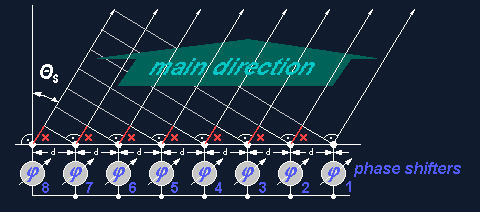
\includegraphics[width=10cm]{gfx/beamSteering.png}
 \caption{Apuntamiento con una conjunto de antena \cite{BeamSteering}.}
 \label{fig:beamSteering}
\end{figure}

Como se puede observar en la figura \ref{fig:beamSteering}, la diferencia de fase entre dos elementos consecutivos,
$\Delta\varphi$, es constante y es llamada incremento de fase \cite{BeamSteering}. Se la puede relacionar con la diferencia
de distancia que tiene que recorrer el haz emitido por cada elemento radiante. Dicha diferencia de distancia se la calcula con
la siguiente relación matemática,


\begin{equation}
	x = d\cdot \sin{\theta_s}
	\label{eq:steering}
\end{equation}

Donde $d$ es la distancia entre dos elementos consecutivos y $\theta_s$ es el apuntamiento deseado del haz emitido. Para calcular
el defasaje de una onda en una cierta distancia $x$, se debe tener en cuenta que depende de su longitud de onda.

\begin{equation}
	\dfrac{2\pi}{\Delta\varphi} = \dfrac{\lambda}{x}
	\label{eq:dist2angle}
\end{equation}

Donde $\Delta\varphi$ es el incremento de fase entre elementos radiantes, $\lambda$ es la longitud de onda transmitida.
Utilizando las ecuaciones \ref{eq:steering} en \ref{eq:dist2angle} se puede obtener el incremento de fase entre RMs contiguos 
necesario para cumplir con el apuntamiento deseado. La ecuación matemática a continuación.

\begin{equation}
	\Delta\varphi = \dfrac{2\pi\cdot d\cdot\sin{\theta_s}}{\lambda}
\end{equation}

\subsection{Calibración interna de una antena polarimétrica}

La respuesta de los componentes varía por el envejecimiento de los mismos al pasar del tiempo, por variaciones de la temperatura
de operación, el manejo imprudente de los mismos, interferencias electromagnéticas (radiadas o conducidas), etc. Dichas 
variaciones deben ser corregidas, buscando que no solo todos los caminos de recepción atenúen y defasen exactamente lo
mismo, sino que también sea un valor conocido. En transmisión el objetivo es el mismo, con la salvedad que se busca que cada
TRM trabaje en su punto de compresión (generalmente cerca de los 6dB) y que la fase de cada elemento depende del apuntamiento
deseado.

Para calibrar la antena por medio de lazos de calibración, la electrónica central se comporta como un VNA (representado en la 
figura \ref{fig:calibrationLoop}). La misma emite una señal por un canal y la compara con lo recibido en el otro canal, 
midiendo el S21 (transmisión directa) de los parámetros S de la antena. Para ello, se debe descontar a la señal recibida, la 
señal emitida. Dicha calibración determina las características de la antena para un determinado instante, si los componentes 
cambian sus características en el tiempo, se debería realizar el proceso de calibración nuevamente para obtener los nuevos 
parámetros S.

\begin{figure}[H]
 \centering
 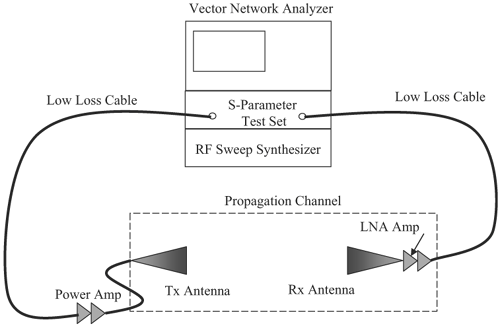
\includegraphics[width=10cm]{gfx/calibrationLoop.png}
 \caption{Lazo de calibración utilizando un VNA \cite{Reed2012}.}
 \label{fig:calibrationLoop}
\end{figure}

La figura \ref{fig:nonCalPattern} muestra la comparación de dos diagramas de radiación de antena, uno calibrado e ideal y el
otro sin calibrar. Se puede observar como los niveles de los lóbulos secundarios y el ancho del lóbulo principal se incrementan.

\begin{figure}[H]
 \centering
 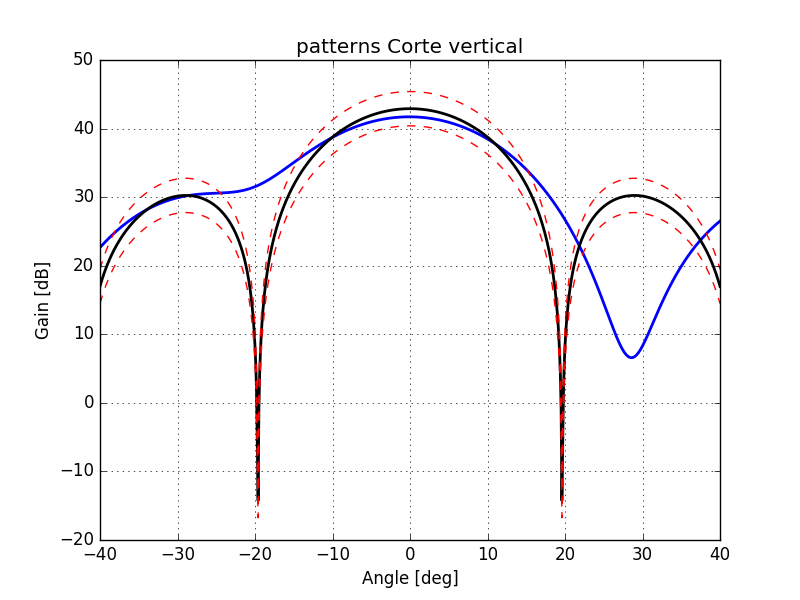
\includegraphics[width=10cm]{gfx/nonCalPattern.png}
 \caption{Diagrama de radiación de antena calibrado vs no calibrado.}
 \label{fig:nonCalPattern}
\end{figure}

\section{Parámetros S de cada componente}

Los componentes que son ideales, se los trata como si estuviesen perfectamente adaptados, logrando así que los coeficientes
de reflexión sean nulos, esto es $S_{11} = S_{22} = 0$. Para mayor información sobre que son los parámetros S ver el apéndice
\ref{sc:appendixSParam}.

\subsection{Elemento Radiante (RM)}

El elemento radiante es un módulo de un único puerto y es pasivo, por lo tanto el parámetro S que lo define es $S_{11}$ y su
valor varía entre -1 y 1.

\begin{itemize}
	\item Cortocircuito ideal: $S_{11} = -1$
	\item Conexión ideal: $S_{11} = 0$
	\item Circuito abierto ideal: $S_{11} = 1$
\end{itemize}

Los casos de cortocircuito y circuito abierto son casos de falla del módulo radiante. Cualquier otro valor intermedio implica
una desadaptación de impedancias.

\subsection{Cable ideal}
Un cable se comporta como una línea de transmisión, y su matriz es la siguiente

$$
\mathbf{S} = \begin{pmatrix} 0 & e^{-\gamma l}\\e^{-\gamma l} & 0\end{pmatrix}
$$

Donde $\gamma = \alpha + j\beta$ es una constante de propagación compleja. $\alpha$ es la atenuación de la línea en [neper/m]
y $\beta = 2\pi/\delta$ con la longitud de onda $\delta$. Para una línea sin pérdidas se obtiene $|S_{21}| = 1$

\subsection{Desplazador de fase ideal}


$$
\mathbf{S} = \begin{pmatrix} 0 & e^{-j\phi_{12}}\\e^{-j\phi_{21}} & 0\end{pmatrix}
$$

Un defasador recíproco posee $\phi_{12} = \phi_{21}$.

\subsection{Atenuador ideal}

$$
\mathbf{S} = \begin{pmatrix} 0 & e^{-\beta}\\e^{-\alpha} & 0\end{pmatrix}
$$

Si el atenuador es recíproco, $\alpha = \beta$. El factor de atenuación, $\alpha$, está en neper. La atenuación en decibeles
viene dado por $A = '20\log_{10}(S_{21})$, $1N = 8.686dB$.


\subsection{Amplificador ideal}

$$
\mathbf{S} = \begin{pmatrix} 0 & 0\\G & 0\end{pmatrix}
$$

Con $G > 1$.


\subsection{Módulo de transmisión recepción ideal}

Dicho componente está compuesto por un defasador ideal junto a un amplificador. Es un componente de tres puertos, el primero 
puede transmisitir o recibir señal, el segundo solamente transmitir y el tercero recibir. Su matriz de parámetros S es la siguiente.

$$
	S_{PSC} = \begin{pmatrix} 0&0&Ge^{-j\phi_{13}} \\ Ge^{-j\phi_{21}}&0&0 \\ 0&0&0\end{pmatrix} 
$$

Este componente se lo puede configurar para unir el primer puerto con el segundo o con el tercero por medio de un interruptor, 
por lo tanto no se lo puede utilizar para transmitir y recibir a la vez. 

\begin{figure}[H]
 \centering
 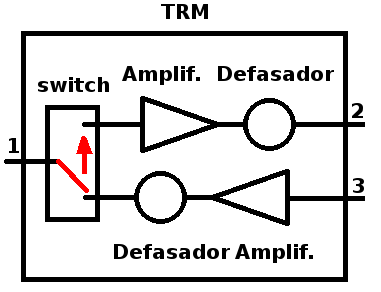
\includegraphics[width=4cm]{gfx/trm.png}
 \caption{módulo de transmisión/recepción}
 \label{fig:trm}
\end{figure}


\subsection{Circulador ideal}

El circulador ideal es sin pérdidas y adaptado en todos sus puertos. La señal entrante por un puerto es exclusivamente
transmitida al puerto siguiente en el sentido de la flecha.

\begin{figure}[H]
 \centering
 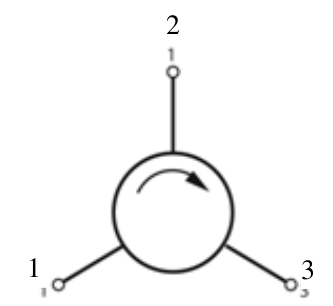
\includegraphics[width=4cm]{gfx/circulator.png}
 \caption{circulador de 3 puertos}
 \label{fig:circulator}
\end{figure}

La matriz de parámetros S es como sigue.

$$
\mathbf{S} = \begin{pmatrix} 0 & 0 & 1\\1 & 0 & 0\\0 & 1 & 0\end{pmatrix}
$$


\subsection{Divisor/Combinador de potencia en RF (PSC)}

El tipo de PSC modelado consiste en una red recíproca y adaptada en todos sus puertos, pero con pérdidas. Puede ser un
componente de 3 o más puertos. A continuación se muestra la matriz de parámetros S genérica para una red de n puertos
(matriz de nxn).

$$
\mathbf{S} = \begin{pmatrix} 0 & \dfrac{1}{n-1} & ... & \dfrac{1}{n-1}\\
							 \dfrac{1}{n-1} & 0 & ... & \dfrac{1}{n-1}\\
							 ... & ... & ... & ... \\
							 \dfrac{1}{n-1} & \dfrac{1}{n-1} & ... & 0 \end{pmatrix}
$$

\subsection{Acoplamientos mútuos}

El acoplamiento mútuo entre módulos radiantes es modelizado con el mismo comportamiento al de un cable, pero con las
propiedades de atenuación y defasaje de una onda en el vacío. Las cuales son:

\begin{equation}
	S12 = S21 = \dfrac{e^{-j\dfrac{\pi}{\lambda}r}}{4\pi r^2}
\end{equation}

siendo r la distancia recorrida por la señal. La matriz de parámetros S resulta,

$$
\mathbf{S} = \begin{pmatrix} 0 & \dfrac{e^{-j\dfrac{\pi}{\lambda}r}}{4\pi r^2}\\\dfrac{e^{-j\dfrac{\pi}{\lambda}r}}{4\pi r^2} & 0\end{pmatrix}
$$

\section{Ejemplo parámetros S}

En esta sección se ejemplifica el armado de las matrices de parámetros S de la antena en una sola polarización desde el punto 
de transmisión a cada elemento radiante. Se asume que se tiene una antena de dos elementos radiantes con la configuración de 
RFDN de la figura \ref{fig:antennaS}. Dicha figura muestra solamente la red de distribución en una sola polarización, para la 
otra polarización, este esquema se repite.

\begin{figure}[H]
 \centering
 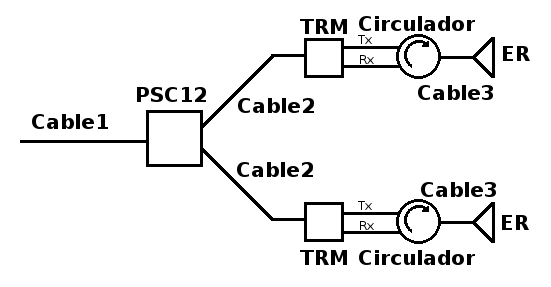
\includegraphics[width=9cm]{gfx/RFDN.png}
 \caption{RFDN para una polarización del esquema de antena.}
 \label{fig:antennaS}
\end{figure}

La tabla \ref{tab:componentSParameters} muestra la cantidad de puertos que posee cada componente y la conexión de cada puerto.

\begin{table}[H]
  \footnotesize
  \centering
  \begin{tabular}{|c|c|p{6cm}|}
	\hline
	\textbf{Componente de Antena} & \textbf{Cantidad de puertos} & \textbf{Notas} \tabularnewline \hline
	cable1 &  2 & \tabularnewline \hline
	\multirow{3}{*}{PSC12} & & Puerto1: conexión cable1 \tabularnewline
	 & 3 & Puerto2: conexión Cable2 (superior) \tabularnewline
	 & & puerto3: conexión Cable2 (inferior) \tabularnewline \hline
	Cable2 & 2 & \tabularnewline \hline
	\multirow{3}{*}{TRM} & & Puerto1: conexión cable2 \tabularnewline
	 & 3 & puerto2: conexión Tx \tabularnewline
	 & & puerto3: conexión Rx \tabularnewline \hline
	\multirow{3}{*}{Circulador} & & Puerto1: conexión Tx \tabularnewline
	 & 3 & puerto2: conexión Cable3 \tabularnewline
	 & & puerto3: conexión Rx \tabularnewline \hline
	Cable3 & 2 & \tabularnewline \hline
	RM & 1 & \tabularnewline \hline
  \end{tabular}
  \caption{Propiedades físicas de cada componente de una antena}
  \label{tab:componentSParameters}
\end{table}

Para la obtención de la respuesta del sistema desde el punto de transmisión/recepción a cada elemento radiante se debe
transformar las matrices de 3 puertos en matrices de 2 puertos. Para ello se deben determinar los puertos de conexión utilizados
para la obtención de dicha matriz asumiendo que se desea obtener la respuesta del sistema de transmisión del elemento radiante
2 (camino en rojo de la figura \ref{fig:antennaSLoop}).

\begin{figure}[H]
 \centering
 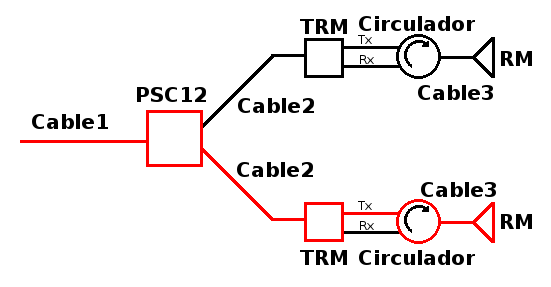
\includegraphics[width=9cm]{gfx/RFDNLoop.png}
 \caption{RFDN para una polarización del esquema de antena. En rojo, cascada de redes de dos puertos.}
 \label{fig:antennaSLoop}
\end{figure}

Como los puertos utilizados por el PSC en el camino rojo de la figura \ref{fig:antennaSLoop} son el 1 y 3, la conversión de
parámetros S resuta ser,

$$
	S_{PSC} = \begin{pmatrix} S11&S12&S13 \\ S21&S22&S23 \\ S31&S32&S33\end{pmatrix} \Rightarrow
	S_{PSC_{13}} = \begin{pmatrix} S11&S13 \\ S31&S33 \end{pmatrix}
$$

Los puertos utilizados por el TRM como el circulador son el 1 y 2, por lo tanto, la conversión de ambos parámetros S resulta
equivalente.

$$
	S_{TRM} = \begin{pmatrix} S11&S12&S13 \\ S21&S22&S23 \\ S31&S32&S33\end{pmatrix} \Rightarrow
	S_{TRM_{12}} = \begin{pmatrix} S11&S12 \\ S21&S22 \end{pmatrix}
$$

$$
	S_{Circulador} = \begin{pmatrix} S11&S12&S13 \\ S21&S22&S23 \\ S31&S32&S33\end{pmatrix} \Rightarrow
	S_{Circulador_{12}} = \begin{pmatrix} S11&S12 \\ S21&S22 \end{pmatrix}
$$

Como se desea caracterizar la respuesta de una cascada de redes de dos puertos, se transforman todas las matrices de cada
componente a parámetros T (ver equaciones \ref{eq:s2t}), se multiplican todas las matrices como se muestra en la ecuación
\ref{eq:cascade} i luego, la matriz resultante se la vuelve a convertir a parámetros S (ver ecuaciones \ref{eq:t2s}).

$$
\begin{aligned}
	S_i &\Rightarrow T_i \\
	T_{in,rm2} &= T_{Cable1}T_{PSC_{13}}T_{Cable2}T_{TRM_{12}}T_{Circulador_{12}}T_{Cable3}T_{RM}\\
	T_{in,rm2} &\Rightarrow S_{in,rm2}
\end{aligned}
$$

Para el caso de querer caracterizar la respuesta inversa de la antena (desde el elemento radiante al receptor) del mismo camino
mostrado en rojo de la figura \ref{fig:antennaSLoop}, el procedimiento es el mismo, salvo que se utilizan los puertos 2 y 3 del
circulador y los puertos 1 y 3 del TRM.

$$
	S_{TRM} = \begin{pmatrix} S11&S12&S13 \\ S21&S22&S23 \\ S31&S32&S33\end{pmatrix} \Rightarrow
	S_{TRM_{13}} = \begin{pmatrix} S11&S13 \\ S31&S33 \end{pmatrix}
$$

$$
	S_{Circulador} = \begin{pmatrix} S11&S12&S13 \\ S21&S22&S23 \\ S31&S32&S33\end{pmatrix} \Rightarrow
	S_{Circulador_{23}} = \begin{pmatrix} S22&S23 \\ S32&S33 \end{pmatrix}
$$

Se vuelven a realizar los pasos de cascada de parámetros T y conversión a parámetros S de la matriz resultante. Pero, como
dicho resultado sigue siendo desde el receptor al módulo radiante, se deben reacomodar los elementos de la matriz

$$
	S_{out,rm2} = \begin{pmatrix} S11&S12 \\ S21&S22\end{pmatrix} \Rightarrow
	S_{rm2, out} = \begin{pmatrix} S22&S21 \\ S12&S11 \end{pmatrix}
$$

%Capítulo 3

\chapter{Procesamiento de la señal de un radar FMCW}
\label{ch:classicalCalibration}
\lhead{\emph{Procesamiento de la señal de un radar FMCW}}
%----------------------------------------------------------------------------------------




Hay distintos tipos de señales con las que se puede transmitir utilizando dicho tipo de radar, las cuales están resumidas en 
el cuadro \ref{tab:signalTypes}.
\todo[inline]{completar la tabla}
\begin{table}[H]
  \footnotesize
  \centering
  \begin{tabular}{|c|c|}
	\hline
	\textbf{Tipo de señal} & \textbf{Característica} \tabularnewline \hline 
	triangular &  1275000000 [Hz] \tabularnewline\hline 
	diente de sierra & 0 [dB] \tabularnewline \hline 
	cuadrada & 0 [deg] \tabularnewline \hline 
	desiredTxPower & 6 [dB] \tabularnewline \hline 
  \end{tabular}
  \caption{Configuración de la antena común para todos los ensayos.}
  \label{tab:signalTypes}
\end{table}

En esta tesis se utiliza el diente de sierra en frecuencia. La figura \ref{fig:sawtoothSignal} ilustra para un caso general los parámetros 
que definen dicha señal, los cuales son el ancho de banda de la señal transmitida ($B$) y el tiempo de repetición de dicho 
pulso ($PRT$).

\todo[inline]{hacer una firgura doble donde muestra la repeticion de chirp y la señal en frecuencia}
\begin{figure}[H]
 \centering
 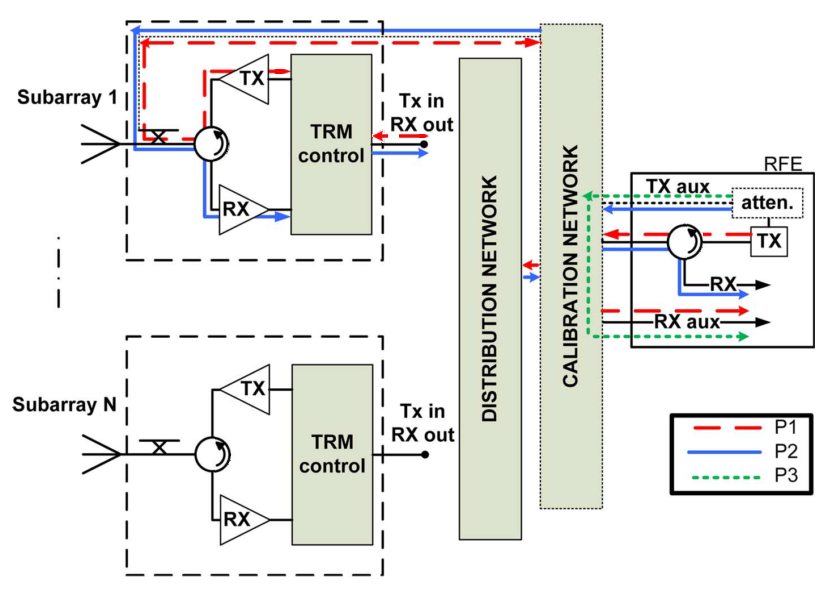
\includegraphics[width=10cm]{gfx/classic_cal_scheme.png}
 \caption{señal diente de sierra en frecuencia.} 
 \label{fig:sawtoothSignal}
\end{figure}

La ecuación que define cada repetición del pulso está descripta a continuación:
\begin{equation}
	f(t) = f_0 + \dfrac{B}{T}(t-\dfrac{T}{2}),\quad 0 \le t < T
	\label{eq:signalFrequency}
\end{equation}

Dado que la fase de una señal es la integral de su frecuencia sumada a una constante, se obtiene la fase instantánea transmitida a partir de
la ecuación \ref{eq:signalFrequency},
\begin{equation}
	\varphi_t(t) = 2\pi f_0t + \dfrac{2\pi B}{2T}(t^2-Tt) + \phi_0,\quad 0 \le t < T
	\label{eq:signalFrequency}
\end{equation}

El eco recibido por un objeto puntual en un rango $R$ y defasando la señal en $\theta$ llega al radar con la fase, 
\begin{equation}
	\varphi_r(t) = w_0(t-\tau) + \dfrac{2\pi B}{2T}((t - \tau)^2-T(t - \tau)) + \theta + \phi_0,\quad 0 \le t < T
	\label{eq:signalFrequency}
\end{equation}

\todo{buscar la e del error}
Donde $\tau=2R\sqrt{e_r}/c$ es el tiempo ida y vuelta de la señal entre el transmisor y receptor del radar.
\todo[inline]{buscar bibliografia del mixer dado que faltan todos los armónicos}
Luego, la señal recibida se la multiplica con la transmitida, por identidad trigonométrica, se obtiene 
\begin{equation}
	x(t) = \dfrac{A_tA_r}{2}(\cos(\varphi_t(t)+\varphi_r(t)) - \cos(\varphi_t(t)- \varphi_r(r)))
	\label{eq:signalFrequency}
\end{equation}

Donde $A_r$ es la amplitud de la señal recibida, la cual es modificada por el ida y vuelta del medio y por el blanco donde se 
genera el eco de la señal.
Que, luego del pasabajos, el término donde está la suma de fases posee una frecuencia de $2w_0$ queda completamente atenuado, 
quedando solamente el término donde está la resta de fases,
\begin{equation}
	x_d(t) = \dfrac{A_tA_r}{2}\cos(w_0\tau + \dfrac{2\pi B\tau}{T}(t - \dfrac{T}{2}) - \dfrac{2\pi B\tau^2}{2T} - \theta)
	\label{eq:signalFrequency}
\end{equation}


Es importante notar que la fase inicial de transmisión se elimina, por lo tanto no importa cual es la fase inicial de cada pulso
transmitido, tampoco importa si varía pulso a pulso dado que se elimina al realizar la mezcla.

Del resultado de la ecuación \ref{eq:signalFrequency} se observa que la fase está compuesta por cuatro términos.
\begin{itemize}
	\item $w_0\tau$ es el término utilizado para determinar distancias con alta precisión en blancos conocidos. \todo{poner 
		referenciaPhase-sensitive FMCW radar system for high-precision Antarctic ice shelf profile monitoring}
	\item $\dfrac{2\pi B\tau}{T}(t - \dfrac{T}{2})$ es un término de fase lineal con el tiempo que representa la frecuencia de la 
		señal.
	\item $\dfrac{2\pi B\tau^2}{2T}$ es un offset en la señal, usualmente pequeño.
	\item $\theta$ es el término de fase originada por el blanco donde incidió la señal transmitida. 
\end{itemize}

Derivando la fase obtenida en la ecuación \ref{eq:signalFrequency} y utilizando la definición de $\tau$, se obtiene la 
frecuencia de dicha señal:
\begin{equation}
	w_d = \dfrac{2\pi B\tau}{T} \rightarrow f_d = \dfrac{2BR\sqrt{e_r}}{cT}
\end{equation}


\begin{comment}
\section{Calibración clásica}

Como fue introducido previamente, una antena es alimentada por un generador y consta de una RFDN y un panel de elementos 
radiantes. Como pueden haber dispersiones en el comportamiento de cada componente, se hace uso de la calibración para 
compensarlas. En particular, este método se lo utiliza para poder medir, detectar y corregir el mal funcionamiento de parte de 
la RFDN, en particular todas las desviaciones se las atribuyen los módulos de Transmisión/Recepción. A su vez, también se 
puede detectar si uno de dichos módulos queda inhabilitado a causa que cierta parte de la cadena de transmisión/recepción 
o dicho componente se destruyó.

Una de las principales limitaciones, esta calibración interna no puede medir las partes pasivas del sistema que están fuera del
lazo de calibración interna (por ejemplo los módulos radiantes), ni la ganancia absoluta, debido a la ausencia de un blanco 
estándar de calibración \cite{Wang2010}.

En la figura \ref{fig:classic_cal_scheme} se muestra el esquema de calibración, en el cual se observan tres modos de
calibración. Cada uno posee distintos caminos, \textbf{P1} (líneas rojas) caracteriza el camino de transmisión, \textbf{P2}
(línea azul) caracteriza el camino de recepción y \textbf{P3} la electrónica central (CE) junto a los puertos auxiliares de
transmisión/recepción. \textbf{P3} es utilizado para corregir posibles variaciones en los pulsos \textbf{P1} y \textbf{P2}
\cite{Makhoul2012}. Se puede apreciar que, para este esquema en praticular, tanto los elementos radiantes como sus cables de 
interconexión quedan fuera de los lazos de calibración.

\begin{figure}[H]
 \centering
 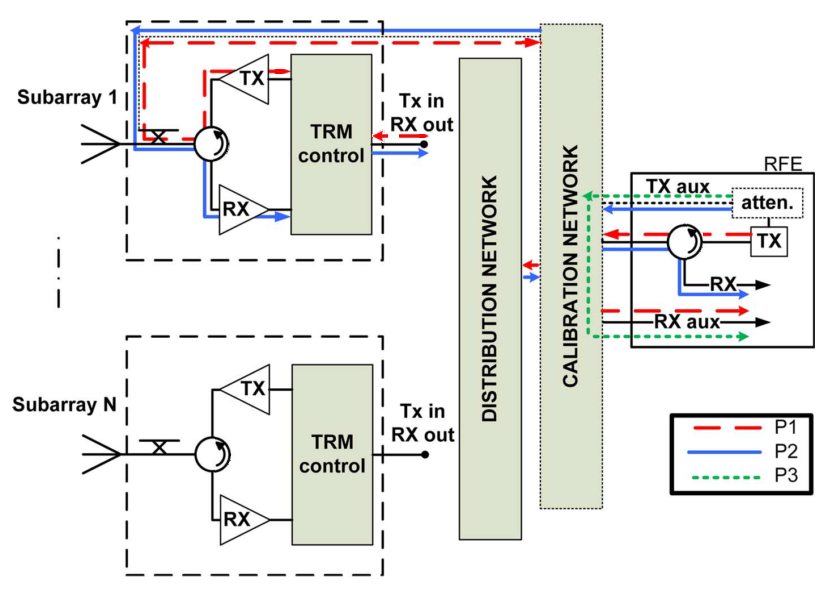
\includegraphics[width=10cm]{gfx/classic_cal_scheme.png}
 \caption{Esquema de calibración interna: camino de calibración de pulsos \textbf{P1} (Tx) en rojo, \textbf{P2} (Rx) en azul
 y \textbf{P3} (electrónica central) en verde \cite{Makhoul2012}.}
 \label{fig:classic_cal_scheme}
\end{figure}

Como ejemplos de satélites que utilizaron dicho método, se los puede nombrar al E-ERS-1, el SIR-C \cite{Curlander1991}, el
terraSAR-X \cite{Schwerdt2005} y el ENVISAT ASAR \cite{Loop}. La figura \ref{fig:calibrMethods} muestra los esquemas
de calibración de los primeros dos sistemas mencionados.

\begin{figure}[H]
	\centering
	\subfloat[]{
		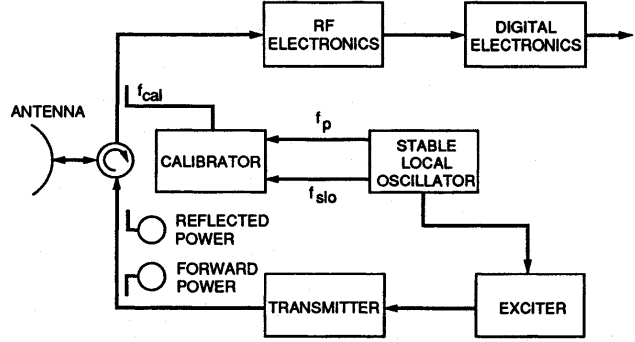
\includegraphics[width=7cm]{gfx/sirCalibration.png}}
 	\subfloat[]{
		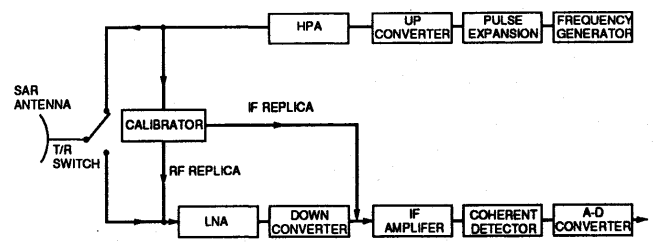
\includegraphics[width=7cm]{gfx/eersCalibration.png}}
	\caption{Esquemas de calibración del SIR-C y E-ERS-1 \cite{Curlander1991}.}
	\label{fig:calibrMethods}
\end{figure}


\subsection{Método} \label{ssc:classicalMethod}

A parte de la medición de la estabilidad del instrumento, es necesario obtener el funcionamiento de los TRMs de forma
individual, dado que el apuntamiento y la planitud de la señal dependen de la configuración de estos componentes. El uso de 
datos de telemetría (por ejemplo, temperaturas y tensiones de los TRMs) junto a una caracterización apropiada en tierra, 
solamente sirve para obtener información limitada del comportamiento de la antena \cite{Br2007}.

Una estrategia para mediciones individuales de cada TRM requiere que el resto de dichos componentes estén apagados. El problema
de esta estrategia es que, al tener parte de la antena apagada, no resulta un método representativo al modo de funcionamiento 
nominal (toda la antena operativa). Para solventar esta problemática y calibrar todos los TRMs a la vez, al menos en 
transmisión o recepción, se hace uso de los defasadores para armar una codificación diferente para cada TRM. En particular, 
por ejemplo, se pueden utilizar los códigos walsh \cite{WalshCode} defasando cada TRM en $\pm90^{\circ}$, siguiendo una 
determinada secuencia $c_{mn}(t)$.

\begin{figure}
 \centering
 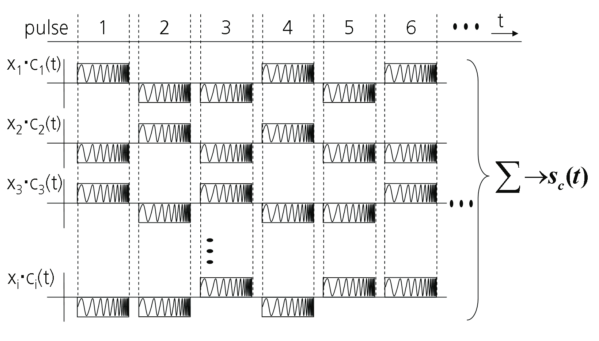
\includegraphics[width=8cm]{gfx/superposition_signals_classic.png}
 \caption{Superposición de señales de todos los TRMs. Cada señal tiene su propia secuencia de código aplicada entre pulsos \cite{Br2007}.}
 \label{fig:sup_sign_classic}
\end{figure}

Por lo tanto, la fase de salida de cada TRM es la fase configurada $\varphi_{mn}$ sumada al defasaje del código de
$90^{\circ}$. Consecuentemente, la superposición de todas las ganancias de los TRMs, $a_{mn}$, y fases, $\varphi_{mn}$,
es obtenida en el puerto de recepción de la RFDN, $s_c(t)$ como se muestra en la figura \ref{fig:sup_sign_classic}.

\begin{equation}
	s_c(t) = \sum_{m=0}^{M-1}\sum_{n=0}^{N-1}c_{mn}\cdot a_{mn}e^{j\varphi{mn}} + n_{mn}
\end{equation}

Donde $n_{mn}$ es el ruido inherente que hay en las mediciones de cada TRM. Para decodificar y obtener la ganancia
$\tilde{a}_{mn}$ y fase estimada $\tilde\varphi_{mn}$ de algún TRM, la señal compuesta $s_c$ es correlacionada con
la secuencia del módulo deseado. Con esta correlación, la modulación de la secuencia se elimina dando como resultado
la ganancia estimada.

\begin{equation}
\begin{aligned}
	\tilde{x}_{mn} &= s_c \otimes c^*_{mn} \\
	\tilde{x}_{mn} = \int s_c(t) &\cdot c^*_{mn}(t) dt = \tilde{a}_{mn}e^{j\tilde{\varphi}_{mn}} \\
\end{aligned}
\label{eq:classic_correlation}
\end{equation}

En general el código de calibración utilizado es el código walsh \cite{WalshCode}. Dicho código deriva de las matrices de 
Hadamard (ver apéndice \ref{AppendixB}); dada sus propiedades de ortogonalidad, cada código, o fila, es unívocamente 
distinguible del resto. Para minimizar la cantidad de mediciones, el largo del código ($l$) debe ser lo más corto positble. 
El número de TRMs de la antena es el determinante de la cota inferior.

\begin{equation}
	l = 2^i \ge N \cdot M
\end{equation}

Siendo $N$ la cantidad de filas y $M$ la cantidad de paneles, o columnas, que tiene el conjunto de antena. No es necesario que
se calibren todos los TRMs de una. Hay tres estrategias que se utilizan con este método de calibración para obtener
distintos niveles de granularidad de mediciones a saber.

\begin{itemize}
	\item \textbf{Nivel módulo:} Este nivel es el que utiliza los códigos más largos, dado que se calibran todos los módulos que
		posee la antena en una polarización determinada ($l = 2^i \ge N \cdot M$).
	\item \textbf{Nivel panel:} En este nivel se utiliza el mismo código para todos los TRMs que son de un mismo panel,
		logrando así, decrecer el largo del código ($l = 2^i \ge M$).
	\item \textbf{Nivel fila:} En este nivel se utiliza el mismo código para todos los TRMs que son de una misma fila,
		logrando así, decrecer el largo del código ($l = 2^i \ge N$).
\end{itemize}

Este método a nivel panel y fila sirve para la caracterización del la configuración del apuntamiento de antena \cite{Br2007}.

\subsection{Problemas y limitaciones}

La calibración clásica fue diseñada para detectar y localizar fallas en los módulos TR permitiendo visualizar como cambia la
fase y atenuación de cada uno a medida que se los comanda a traves de una electrónica central. Como contracara, adolece de
los siguientes problemas:

\begin{itemize}
	\item Caracterización previa de los elementos de antena: Para poder conocer la ganancia del lazo de transmisión o recepción
es necesario conocer la potencia de la señal de calibración, para sustraerla del resultado obtenido. El lazo de calibración
donde se realiza esta medición es el que se muestra en la imagen \ref{fig:classic_cal_scheme}, llamado \textbf{P3}. En esta
medición no se puede determinar cuanto atenúa el lazo, por lo tanto se opta por caracterizar en tierra dichos componentes
para las frecuencias y temperaturas de trabajo.
	\begin{itemize}
		\item Costo de materiales: Materiales caracterizados en temperatura valen el doble que los no caracterizados, 
			dado que no es un trabajo sencillo y requiere el uso de cámaras de termovacío para realizar los ensayos.
		\item Costo de recursos: La campaña de caracterización puede durar meses, con equipos de trabajo dedicados, lo cual implica
			un gasto de dinero muy importante.
		\item Comportamiento de materiales fin de vida: Como el material envejece, cambia sus propiedades, por lo tanto las mediciones realizadas
			en la campaña de caracterización dejan de tener validez.
	\end{itemize}
	\item Complejidad del hardware de la antena: Como se calibra solo una parte de la antena por vez, transmisión o recepción en
		una u otra polarización (H o V), es necesario que el lazo de calibración esté compuesto por la parte de la antena a
		calibrar junto a hardware dedicado (cables y switches) a esta tarea. Logrando así, no solo que la construcción de la antena
		sea más compleja y que se tengan que caracterizar más componentes, sino también que el defasaje y atenuación que este
		hardware dedicado posee es atribuido a los TRMs, añadiendo así más error en la medición.
	\begin{itemize}
		\item Acoplamiento: Como hay hardware agregado, el diseño tiene que se más complicado dado que se incrementan los posibles
			acoplamientos entre componentes.
	\end{itemize}
	\item Inestabilidad del generador: Este método es sumamente susceptible a las variaciones de fase y potencia del generador
		entre pulsos de calibración. Por lo tanto, es de vital importancia armar un generador que sea sumamente estable.
	\item Sistema incompleto: Como hay componentes que están fuera de los lazos de calibración, con el método nunca se puede
		determinar de forma totalmente correcta la ganacia de la antena en cualquiera de sus modos.
	\item A la hora de elegir la longitud del código Walsh, es importante que siempre haya un elemento radiante virtual en la
		antena para evitar la primer columna de la matriz de códigos. En caso contrario el primer TRM siempre tendrá un error en
		la estimación de su ganancia \cite{Wang2010}.
	\item Pérdida de ortogonalidad en el código utilizado por comportamiento de defasadores: Si el defasador no tiene un
		comportamiento exactamente igual al configurado a la hora de realizar la calibración, los códigos walsh pierden
		ortogonalidad y, por ende, se logra obtener una mala estimación de los valores de ganancia de la antena.
    \item Compensacion de temperatura en elementos: Se debe mantener la temperatura de los elementos en los valores
        caracterizados para garantizar que las calibraciones sirven.
    \item Es completamente dependiente del modelo y análisis térmico. Por ejemplo, se asume que el comportamiento de los
        elementos radiantes de la antena no varían con la temperatura.
\end{itemize}
\end{comment}

%\chapter{Calibración utilizando acoplamientos mútuos}
\label{ch:convertidores}
\lhead{\emph{Calibración utilizando acoplamientos mutuos}}

\section{Calibración utilizando acoplamientos mutuos}

El método que utiliza los acoplamientos mutuos toma ventaja del acoplamiento mutuo inherente de un conjunto transmitiendo
y recibiendo entre elementos adyacentes. Para llevar a cabo dicho método, este tipo de antenas debe cumplir un
requerimiento muy importante que es poder transmitir con un elemento y simultáneamente recibir con otro sin que se sature o peor
aun, que se queme. Normalmente, este requerimiento implica separar las redes de transmisión y recepción \cite{Gao2001}. Para 
antenas que no cumplen la separación de la redes de transmisión y recepción se puede transmitir en una polarización y recibir
en otra. Por ende, es requisito para poder implementar el método que la red utilizada permita seleccionar los TRMs que van a 
estar en transmisión, en recepcion y en modo protegido. De esta forma, se establecen zonas en las cuales puede aplicarse el 
método actual dado que los niveles no son tan altos como para quemarlos ni tan bajos como para que no se alcance un nivel 
necesario para calibrar. La figura \ref{fig:levels} ejemplifica las tres zonas de recepción al emitir con un elemento radiante:
\begin{itemize}
	\item En rojo: zona de acoplamiento destructivo. Los TRMs deben estar protegidos.
	\item En verde: zona de acoplamiento dentro de los límites aceptables para aplicar el método.
	\item En azul: zona de acoplamiento débil. No se puede aplicar el método dado que el nivel de señal es inferior al piso de 
		ruido. 
\end{itemize}

\begin{figure}[H]
 \centering
 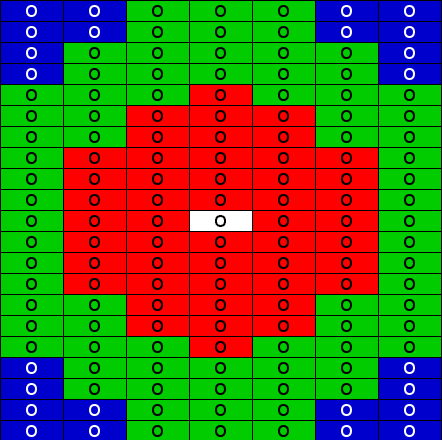
\includegraphics[width=9cm]{gfx/mutualCouplingLevels.png}
 \caption{Niveles de recepción de la antena al emitir con un elemento. En rojo, acoplamiento destructivo; en verde, 
 acoplamiento admisible y en azul acoplamiento débil.}
 \label{fig:levels}
\end{figure}

Para evitar que los elementos que no conforman parte del lazo activo de calibración interfieran, inyectando ruido en las redes 
de transmisión y/o recepción, se los debe poder configurar en modo alta impedancia (en este modo no se transmite ni recibe 
señal). En la figura \ref{fig:mutual_general} se puede observar un ejemplo.

\begin{figure}[H]
 \centering
 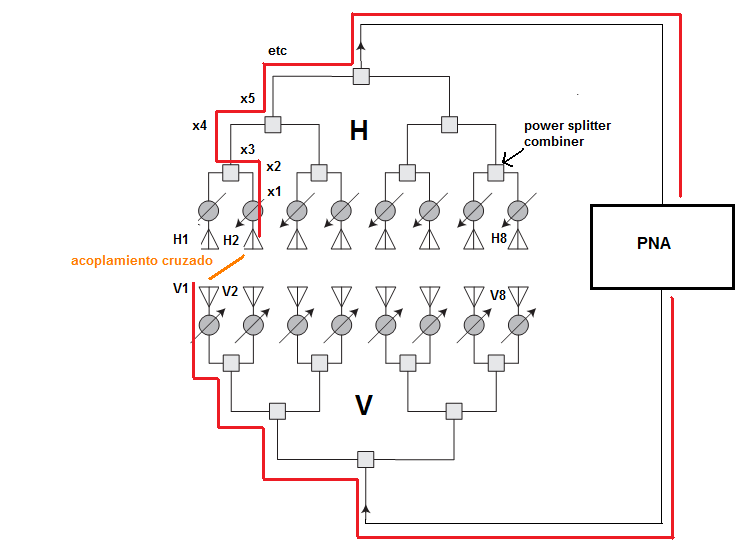
\includegraphics[width=9cm]{gfx/mutualCouplingExample.png}
 \caption{Ejemplo de calibración utilizando acoplamientos mutuos, transmitiendo en polarización V y recibiendo en H}
 \label{fig:mutual_general}
\end{figure}

En la figura \ref{fig:mutual_general} se puede observar un ejemplo en donde se transmite desde el elemento $e_1$ en 
polarización horizontal (H) y se recibe con el elemento $e_0$ en polarización vertical (V). Si se repite el proceso
secuencialmente con todos los elementos de recepción y luego con todos los elementos de transmisión, se puede determinar a
priori tanto la potencia de transmisión como la de recepción y lo que atenúa cada acoplamiento mutuo.

Como un primer paso, se determina que la cantidad de incógnitas que tiene una antena de $m$ elementos por $n$ paneles. Como
se puede transmitir y recibir en dos polarizaciones (H y V), la antena cuenta con $4MN$ incógnitas de RFDN (2 por Tx en H/V y
otras 2 por Rx en H/V). A su vez, en el apéndice \ref{AppendixA} se realiza el cálculo de la cantidad de acoplamientos mutuos
que posee una antena polarimétrica, particularmente, la ecuación \ref{eq:amountMutCoupling} muestra la cantidad de
incógnitas, que, para este caso, resulta ser de $MN(MN-1)/2$. Totalizando en $MN(MN + 7)/2$ incógnitas.

Asumiendo que se transmite de a un RM por lazo de calibración, a priori, se dispone de un máximo de $(MN)^2$ ecuaciones por
polarización a transmitir. Totalizando en $2(MN)^2$. Para que el sistema tenga solución, la cantidad de ecuaciones debe ser
mayor a la de las incógnitas, por lo tanto, la cantidad mínima de elementos radiantes es de

$$
\begin{aligned}
	2(MN)^2 &\ge  \dfrac{MN(MN + 7)}{2} \\
	4MN &- MN \ge7 \\
	MN &\ge \dfrac{7}{3}
\end{aligned}
$$

Como $M$ y $N$ son números enteros, con que la antena tenga tres o más elementos radiantes, ya se puede utilizar el método.

La herramienta matemática utilizada para resolver el sistema de ecuaciones es el de los cuadrados mínimos,
ver apéndice \ref{AppendixB}, con el cual se obtiene la aproximación que tenga menor error cuadrático medio.

Ante la posibilidad que no siempre se cuente con el tiempo necesario para generar todos los lazos de calibración necesarios
para calibrar la antena en el modo presentado, tres modalidades serán presentadas para este método.

\begin{itemize}
	\item \textbf{Modo completo:} En esta modalidad no solo se estima la ganancia en transmisión y recepción en ambas
		polarizaciones (H y V), sino que también se determinan los acoplamientos mutuos de la antena. La cantidad de ecuaciones necesarias es
		de $MN(MN + 7)/2$.
	\item \textbf{Modo rápido:} En esta modalidad se estima la ganancia en transmisión y recepción em ambas polarizaciones
		(H y V) utilizando el valor guardado de la planitud de la antena calculado previamente. La cantidad de ecuaciones necesarias
		es de $4MN$.
	\item \textbf{Modo planitud ideal:} Esta modalidad es igual al modo rápido, asuminedo que la antena es perfectamente plana.
		La cantidad de ecuaciones necesarias es de $4MN$.
\end{itemize}


\subsection{Método}

Asumiendo que se transmite desde el elemento $e_m$ y se recibe desde el $e_n$, la función de transferencia del lazo de
calibración está compuesta por:

\begin{itemize}
	\item La configuración de atenuación y defasaje de los defasadores y atenuadores, tanto de transmisión como de recepción,
		denotados como $w_{Tm}(i)$ y $w_{Rn}(j)$, donde $i$, $j$ son las diferentes posibles configuraciones.
	\item La atenuación y defasaje combinados por los cables, conectores, divisores y combinadores de potencia, módulos radiantes
		y defasadores, denotados como $u_{Tm}$ y $u_{Rn}$.
	\item El acoplamiento mutuo entre los elementos participantes, denotado como $C_{m, n}$.
\end{itemize}

Por lo tanto, la función de transferencia completa resulta,

\begin{equation}
	C^{'}_{m,n} = w_{Tm} u_{Tm} C_{m,n} w_{Rn} u_{Rn}
	\label{eq:transfer_mn}
\end{equation}

Si se transmite con el mismo elemento, $e_m$, pero se recibe con otro, $e_{n + 1}$, la transferencia resulta

\begin{equation}
	C^{'}_{m,n + 1} = w_{Tm} u_{Tm} C_{m,n + 1} w_{Rn + 1} u_{Rn + 1}
	\label{eq:transfer_mn1}
\end{equation}

Tomando la relación de ambas transferencias \ref{eq:transfer_mn} y \ref{eq:transfer_mn1},

\begin{equation}
	W^{m}_{Rn,n + 1} = \dfrac{C^{'}_{m,n}}{C^{'}_{m,n + 1}} = \dfrac{C_{m,n} w_{Rn} u_{Rn}}{C_{m,n + 1} w_{Rn + 1} u_{Rn + 1}}
\end{equation}

Se asume que el valor del acoplamiento depende de dos factores a saber. El primero es por comunicar los elementos utilizando
polarizaciones cruzadas, y dicha atenuación es constante para cualquier elemento. El segundo, es debido a la atenuación y
defasaje de la señal que viaja en el vacío, por lo tanto, depende exclusivamente de la distancia que hay entre los elementos
a comunicar.

Ahora, si se combinan las funciones de transferencia $C^{'}_{m,n+1}$ y $C^{'}_{m,n+2}$, la relación resulta,

\begin{equation}
	W^{m}_{Rn + 1,n + 2} = \dfrac{C^{'}_{m,n+1}}{C^{'}_{m,n+2}} = \dfrac{C_{m,n+1} w_{Rn+1} u_{Rn+1}}{C_{m,n + 2} w_{Rn + 2} u_{Rn + 2}}
\end{equation}

Ahora, si se combinan las funciones de transferencia $C^{'}_{m,n}$ y $C^{'}_{m,n+2}$,

\begin{equation}
	W^{m}_{Rn,n + 2} = \dfrac{C^{'}_{m,n}}{C^{'}_{m,n + 2}}\cdot\dfrac{C^{'}_{m,n+1}}{C^{'}_{m,n+1}} = W^{m}_{Rn,n+1}\cdot W^{m}_{Rn+1,n + 2}
\end{equation}

Generalizando, se pueden obtener todos los lazos de calibración en función de uno,

\begin{equation}
	W^{m}_{R0,k} = \prod_{i=0}^{k-1} W^{m}_{Ri,i+1} = \prod_{i=0}^{k-1}\dfrac{C^{'}_{m,i}}{C^{'}_{m,i+1}} =
		\prod_{i=0}^{k-1}\dfrac{C_{m,i} w_{Ri} u_{Ri}}{C_{m,i + 1} w_{Ri + 1} u_{Ri + 1}}
	\label{eq:rx_cal}
\end{equation}

Si se realiza la misma deducción, pero en vez de transmitir siempre con el mismo elemento, se lo utiliza para recibir, se obtiene

\begin{equation}
	W^{m}_{T0,k} = \prod_{i=0}^{k-1} W^{m}_{Ti,i+1} = \prod_{i=0}^{k-1}\dfrac{C^{'}_{i,m}}{C^{'}_{i+1, m}} =
		\prod_{i=0}^{k-1}\dfrac{w_{Ti} u_{Ti} C_{i,m}}{w_{Ti + 1} u_{Ti + 1}C_{i + 1, m}}
	\label{eq:tx_cal}
\end{equation}

Analizando las ecuaciones \ref{eq:rx_cal} y \ref{eq:tx_cal}, dos conclusiones inmediatas se deducen. La primera es que el
resultado no es único, por lo tanto, en principio, con este método no se pueden obtener ganancias absolutas (de transmisión,
recepción y acoplamientos mútuos), solamente ganancias relativa entre dichos elementos. La segunda, es que el sistema tiene
dos grados de libertad, en otras palabras, para poder obtener la ganancia absoluta de todo el sistema, es necesario agregar
dos ecuaciones más que definan algún valor pertenenciente a dos de los tres conjuntos de incógnitas.

Si se asume que a misma distancia el acoplamiento es el mismo o si se los reutilizan de una calibración anterior, las
ecuaciones \ref{eq:rx_cal} y \ref{eq:tx_cal} se simplifican, logrando que la cantidad de incógnitas se reduzca habilitando
de esta forma los métodos rápidos y de planitud ideal. 

Como es necesaria una menor cantidad de ecuaciones de calibración, la estrategia a encarar es la de utilizar lazos simétricos
con un elemento en común. Al restar ambos caminos, no solo se elimina la RFDN común, sino que también se elimina el
acoplamiento mútuo. La cantidad de estos lazos termina siendo determinada como una solución de compromiso entre la cantidad de
mínima necesaria para poder utilizar el método y la cantidad de ecuaciones redundantes para disminuir la incertidumbre en el
resultado. Las ecuaciones para recepción y transmisión simplificadas resultan.

\begin{equation}
	W^{'}_{R0,k} = \prod_{i=0}^{k-1} W^{'}_{Ri,i+1} = \prod_{i=0}^{k-1}\dfrac{w_{Ri} u_{Ri}}{w_{Ri + 1} u_{Ri + 1}} =
	\dfrac{w_{R0} u_{R0}}{w_{Rk} u_{Rk}}
	\label{eq:rx_simp_cal}
\end{equation}

\begin{equation}
	W^{'}_{T0,k} = \prod_{i=0}^{k-1} W^{'}_{Ti,i+1} = \prod_{i=0}^{k-1}\dfrac{w_{Ti} u_{Ti}}{w_{Ti + 1} u_{Ti + 1}} =
	\dfrac{w_{T0} u_{T0}}{w_{Tk} u_{Tk}}
	\label{eq:tx_simp_cal}
\end{equation}

Si el RM común se utiliza para transmitir la señal, se obtienen ecuaciones para calibrar la parte de recepción, en cambio,
si se lo utiliza para recibir la señal, se calibra transmisión. La figura \ref{fig:ideal_strategy} esquematiza esta estrategia.

\begin{figure}[H]
 \centering
	\subfloat[]{
		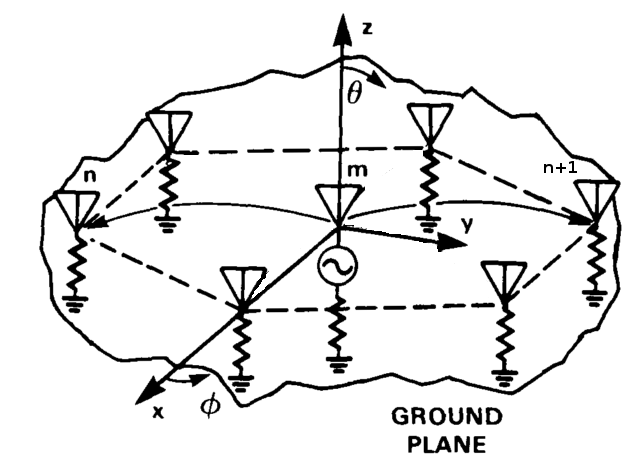
\includegraphics[width=5cm]{gfx/mutualRxCal.png}}
	\subfloat[]{
		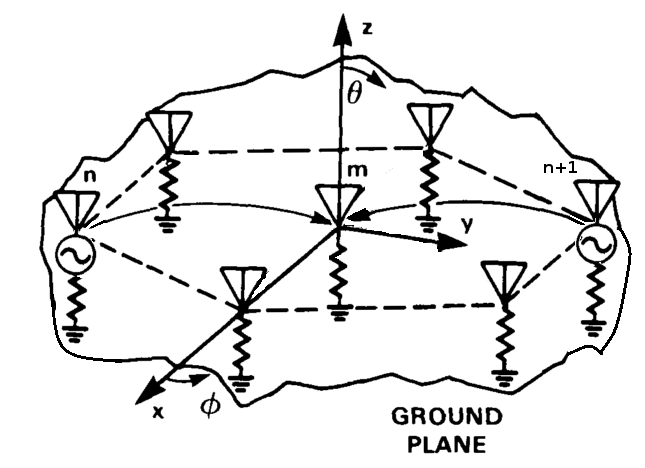
\includegraphics[width=5cm]{gfx/mutualTxCal.png}}
	\caption{estrategia de planitud ideal. (a) Calibra lazos de recepción, (b) Calibra lazos de transmisión \cite{Aumann1989}.}
 \label{fig:ideal_strategy}
\end{figure}

\subsection{Determinación de la fase} \label{ssc:mutualPhase}

Como el método de resolución utilizado en este método es de naturaleza lineal, resolviendo ecuaciones del estilo $Ax = b$, y
como la fase de una señal es de naturaleza modular, de 360 grados, se pueden cometer errores en la resolución. Dependiendo de
como sea $A$ y que valores tenga $x$, $b$ no necesariamente está contenido dentro del conjunto solución (en módulo 360)
generando así un error en la resolución de la estimación del valor $x$.

Para ejemplificar, se asume que se tiene un conjunto de antena de tres elementos radiantes. La RFDN (en Tx y Rx) defasa 100
grados, el defasador del primer elemento está configurado en 240 grados y el del tercero en 120, el acoplamiento mutuo no defasa
y se utiliza la ecuación $\dfrac{C^{'}_{1,2}}{C^{'}_{3, 2}}$. La figura \ref{fig:phaseDetermination} muestra la antena con los 
lazos de calibración utilizados.

\begin{figure}[H]
 \centering
 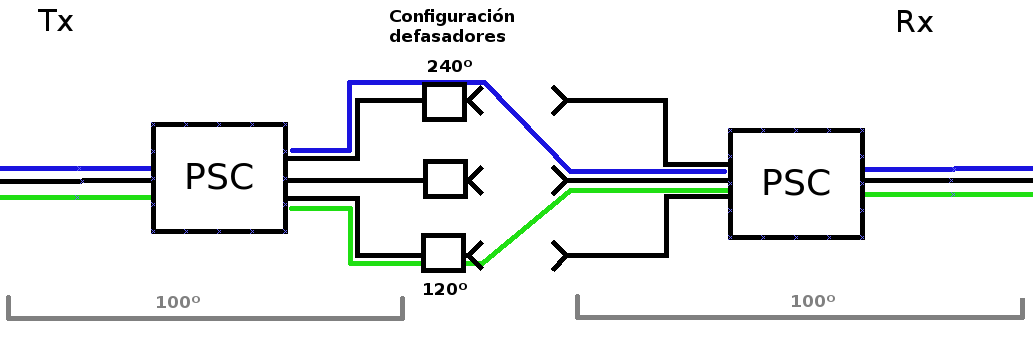
\includegraphics[width=10cm]{gfx/loopCal.png}
 \caption{Lazo de calibración de una antena polarimétrica}
 \label{fig:phaseDetermination}
\end{figure}

Utilizando la ecuación previamente mencionada, $A$ resulta ser
$$
	\mathbf{A} = \begin{pmatrix} 1 & 0 & -1\end{pmatrix}
$$
El verdadero valor de x resulta ser la contribución de la rama de transmisión junto a la configuración del defasador del TRM,
$$
	\mathbf{x} = \begin{pmatrix} 340 \\ x \\ 220\end{pmatrix}
$$

Al resolver la ecuación $Ax$ se obtiene el resultado de 120 grados. Si la fase fuese de naturaleza lineal, este sería el valor 
resultante de la resta de la medición de ambos lazos de calibración. Las mediciones de dichos lazos resultan: 
\begin{itemize}
	\item La fase de $C^{'}_{1,2}$ es 440 grados, en módulo 360 resulta igual a 80 grados (100 grados por la rama de
		transmisión sumado a 240 por el defasador del primer TRM y 100 grados más por la rama de recepción).
	\item La fase de $C^{'}_{3, 2}$ es 320 grados (100 grados por la rama de transmisión sumado a 240 por el defasador
		del primer TRM y 100 grados más por la rama de recepción).
\end{itemize}

La resta de dichas mediciones deberían ser igual a 120 grados, pero se observa que es igual a -240 grados generando así un
error en la estimación de la fase.

Para soluciona esto, la estrategia propuesta es la de reutilizar el valor estimado de $x$ de una calibración previa, calcular
el $b$ ideal y modificar los valores de $b$ de la calibración actual sumando o restando de a 360 grados para acercarse lo más 
posible a dichos valores esperados. Para la primera calibración, es necesario medir cuanto defasa la antena en al menos una 
rama punta a punta. 

\subsection{Problemas y limitaciones}

La mayor limitación de este método es que es necesario conocer, a groso modo, el valor del defasaje de uno de los caminos de
Tx o Rx punta a punta. Esto es para poder evitar errores de cálculos al obtener la fase de transmisión o recepción del
sistema, ya que la misma tiene un comportamiento modular. Dicho valor solo se lo utilizará una vez, dado que ya para las
subsiguientes calibraciones, el valor previo de fase de la antena es conocido y reutilizado. 

Para obtener dicho valor inicial, se puede utilizar la fase delvuelta por el método de calibración clásica o se puede realizar
una medición de campo cercano en temperatura, emitiendo sólamente con un elemento radiante para deducir la fase de la red de 
transmisión, para obtener el defasaje de la red de recepción, se emite con un elemento externo y se recibe con solo un elemento
radiante. 

%\chapter{Modelización}
\label{ch:modelizacion}
\lhead{\emph{Modelización}}

\section{Modelo de la antena}

El modelo de antena está programado de tal forma que se lo pueda utilizar para simular una antena con parámetros de RF,
la misma está conformada por los siguientes componentes: cables, psc, trms, defasadores y elementos radiantes. 

La modelizaci\'on de los componentes en RF se realiza utilizando los par\'ametros S. En el apéndice \ref{AppendixC} se muestra 
un ejemplo de estos archivos para una antena de dos elementos radiantes.

Como es necesario realizar ensayos de montecarlo utilizando disitntos tipos de calibraciones ante una misma configuración y 
comportamiento de antena, se optó por guardar en disco dicha información utilizando archivos json. En los cuales se guarda la
configuración y propiedades físicas tanto del panel como de la RFDN. Las propiedades del primer grupo son, simplemente, las 
distancias entre todos los elementos. Las del segundo grupo corresponden a la matriz de parámetros S y la interconexión entre 
componentes. En el anexo \ref{AppendixC} se puede observar un ejemplo de estos archivos para una antena con dos elementos 
radiantes.

Dado lo mencionado previamente, el simulador consta de dos etapas, la primera parte es la encargada de la modelización
de la antena y sus componentes; y la segunda, de calibrar dicho modelo. La figura \ref{fig:prog_inic} muestra de forma 
simplificada el flujo de ejecuci\'on del programa.

\begin{figure}
 \centering
 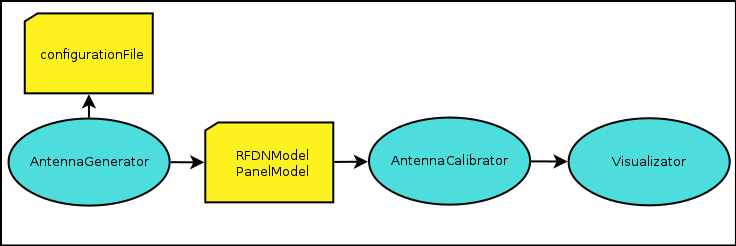
\includegraphics[width=10cm]{gfx/FlujoEjecucion.png}
 \caption{Flujo de ejecuci\'on del modelo de antena.}
 \label{fig:prog_inic}
\end{figure}


\subsection{Generador de Antena}

En principio, una antena necesita que todos los caminos entre el punto donde se inyecta o recibe la se\~nal y los m\'odulos 
radiantes sean iguales. Esta caracter\'istica es similar a la de un \'arbol balanceado. Por lo tanto, para definir la 
estructura interna de la antena, se definen simplmenete los elementos que conforman dicho \'arbol y, para determinar el orden 
de armado de la antena, se utiliza una lista. El orden es descendiente, si se para en un elemento de la lista, los de la 
izquierda son ascendientes y los de la derecha son descendientes. En la figura \ref{fig:2RMAntenna} se muestra la antena que 
se construye teniendo como configuración: [\enquote*{cable1}, \enquote*{psc12}, \enquote*{cable2}, \enquote*{trm}, 
\enquote*{circulator}, \enquote*{cable3}, \enquote*{rm}].

\begin{figure}
 \centering
 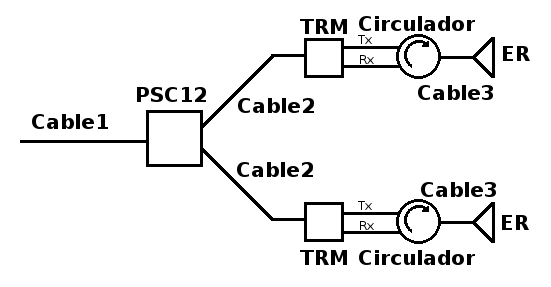
\includegraphics[width=10cm]{gfx/RFDN.png}
 \caption{Estructura interna de una de las polarizaciones de una antena con dos elementos radiantes.}
 \label{fig:2RMAntenna}
\end{figure}

Es necesario definir las características físicas de cada uno de los elementos que componen la antena. La tabla 
\ref{tab:propertiesOfComponents} determina las propiedades de cada uno.

\begin{table}[H]
  \footnotesize
  \centering
  \begin{tabular}{|c|c|}
	\hline
	\textbf{Componente de Antena} & \textbf{Cacarcterísticas físicas} \tabularnewline \hline 
	\multirow{2}{*}{cable} &  attenuation [db] \tabularnewline \cline{2-2}
	 & length [m] \tabularnewline \hline 
	\multirow{3}{*}{TRM} & isDead \tabularnewline \cline{2-2}
	 & gain [db]\tabularnewline \cline{2-2}
	 & phaseShift [deg] \tabularnewline \hline 
	PSC1$j$ & outputPorts = $j$ \tabularnewline \hline 
	circulator & \tabularnewline \hline 
	RM & \tabularnewline \hline 
  \end{tabular}
  \caption{Propiedades físicas de cada componente de una antena}
  \label{tab:propertiesOfComponents}
\end{table}

Como es necesario que la representación de las propiedades mencionadas previamente sean representativas en radio frecuencia,
se utilizan los parámetros S (como se menciona en el capítulo \ref{ch:phasedArray}). En la figura \ref{fig:creationPackage} 
se muestra el diagrama de clases donde se puede observar que el creador de antena hace uso de los generadores de parámetros S 
de cada componente.

\begin{figure}
 \centering
 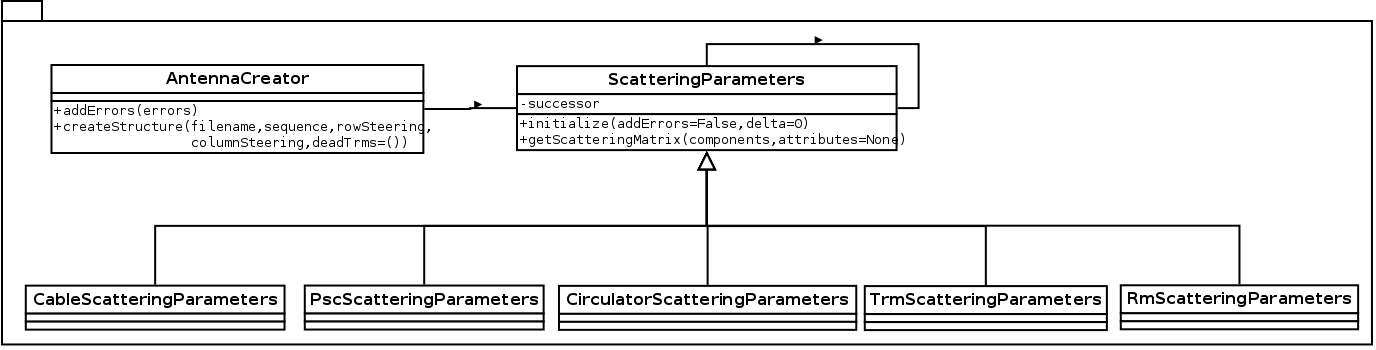
\includegraphics[width=15cm]{gfx/creationPackage.png}
 \caption{Diagrama de clases del generador de antena.}
 \label{fig:creationPackage}
\end{figure}

Con la RFDN, si bien está definida la cantidad de elementos radiantes, falta definir las dimensiones de la antena, 
en otras palabras, la cantidad de paneles, la cantidad de elementos por panel y la separación, tanto horizontal como vertical,
entre elementos. Los primeros se traducen a cantidad de columnas y filas de RMs. 

Como dicha información es redundante y posiblemente incompatible con la definición de la estructura interna de la antena, es 
necesario un chequeo de compatibilidad. La figura \ref{fig:frontAntenna} muestra el frente de una antena que se construye 
teniendo como configuración: "quantityRows": 1, "quantityColumns": 2, "verticalSeparation": 0.2 y "horizontalSeparation": 0.2.

\begin{figure}
 \centering
 
\includegraphics[width=4cm]{gfx/FrontAntenna2.png}
 \caption{Frente de antena de dos elementos radiantes.}
 \label{fig:frontAntenna}
\end{figure}

Una vez obtenida la estructura de la antena, es necesario determinar que componentes van a tener desvíos en el comportamiento 
deseado. Para ello, se agrega una lista indicando los componentes con errores. Las incertidumbres tienen una distribución 
gaussiana con media 0. El desvío estandar es configurable.

Si se deseara realizar la calibración en modo completo, se deberían agregar errores de planitud de la antena. Con lo cual, 
dichos desvíos se verían reflejados en el archivo de la configuración del panel de la antena. En la presente tesis solamente 
se desarrolló el modelo con planitud ideal.

\subsection{Calibrador}

En la figura \ref{fig:modelPackage} se muestra el diagrama de clases del calibrador del modelo de antena. Se puede observar que
la clase Antena, la cual pertenece al modelo, modeliza el comportamiento de todos sus componentes. Los calibradores pueden ser 
el clásico o el de acoplamientos mútuos; el primero utiliza un creador de señales chirp y de códigos walsh, en cambio, el 
segundo utiliza clases del tipo MatrixCalibratorBuilder, las cuales tienen distintas estrategias para generar ecuaciones en base
a los lazos de calibración generados.

\begin{figure}
 \centering
 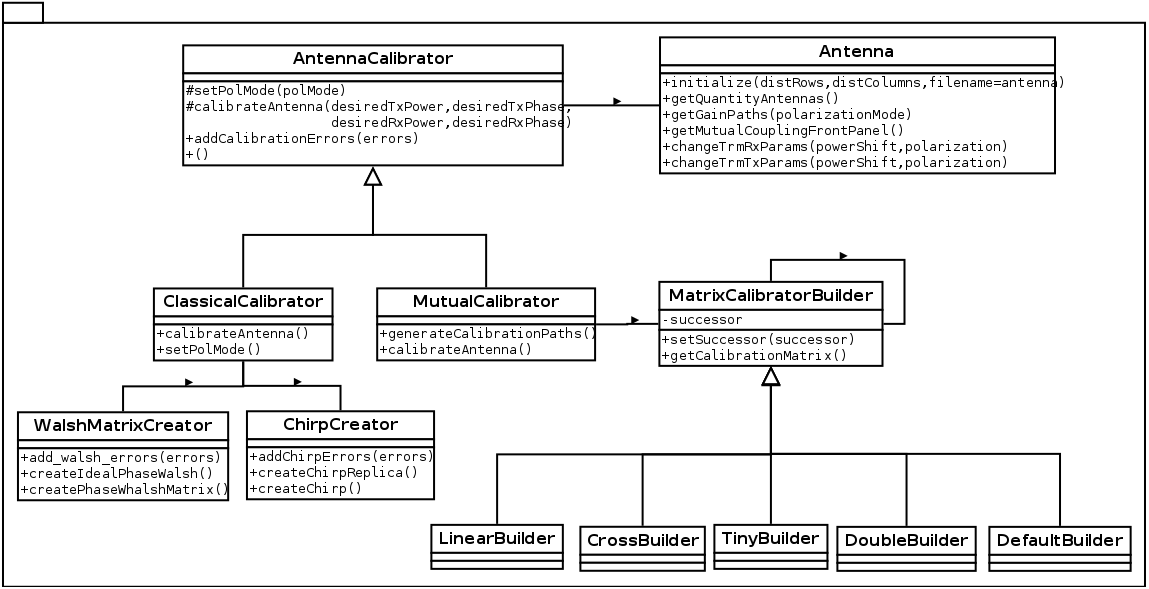
\includegraphics[width=15cm]{gfx/modelPackage.png}
 \caption{Diagrama de clases del calibrador de antena.}
 \label{fig:modelPackage}
\end{figure}


A la hora de calibrar, los primeros parámetros a definir son la potencia (en dB), fase (en grados) y frecuencia (en Hz) de la 
señal utilizada con que se alimenta la antena para ser transmitida. A su vez, se debe definir el apuntamiento deseado. Para 
ello, se tienen que configurar la fase de los defasadores en transmisión de la polarización a transmitir, tomando en cuenta lo 
explicado en la sección \ref{ssec:beamSteering}. Estos valores están definidos en el archivo de configuración bajo el nombre 
de \enquote*{Row Steering} y \enquote*{Column Steering}. Los mismos se traducen como el apuntamiento vertical y horizontal 
respectivamente de la antena.

Una vez definidos los parámetros previamente mencionados, se puede obtener la ganancia de la antena en las partes de 
transmisión y recepción para crear los lazos de calibración. Dichas ganancias están definidas como matrices de parámetros
S y se las obtiene realizando los siguientes pasos.

\begin{enumerate}
	\item Se recorre recursivamente la estructura de la antena, se van leyendo los parámetros S de cada componente y se va 
		armando una lista de caminos distintos.
	\item Si el componente tiene más de un puerto de salida, se agranda la lista de elementos encontrados. La lista final tiene 
		tantos elementos como RMs tiene la antena.
	\item A la matriz leída se la transforma en parámetros T utilizando la transformación definida en la sección 
		\ref{ssec:conversion} y se la multiplica con los datos guardados en la lista de elementos encontrados. Se realiza esto 
		por la propiedad de multiplicación entre matrices de transferencia definida en la sección \ref{ssec:transMatrix}.
	\item Una vez recorrida toda la antena, la lista de parámetros T se la convierte nuevamente a parámetros S.
	\item Si los parámetros S son para recepción de la antena, se deben intercambiar los elementos de la matriz. $S_{11}$ con 
		$S_{22}$ y $S_{21}$ con $S_{12}$.
\end{enumerate}

Para armar los lazos de calibración, se tiene que tener en cuenta distintos tipos de errores que pueden afectar a los mismos, 
los cuales son: error de ganancia entre pulsos, error de ganancia de la chirp replica y error de fase del walsh. Todos estos 
errores son tratados como gaussianos con media igual a cero.

Desvíos de ganancia o fase entre pulsos: Esta incertidumbre se puede dar por inestabilidades en el oscilador local que genera 
la señal a transmitir/calibrar la antena o incertidumbres de medición del receptor.

Desvíos de ganancia o fase de la chirp replica: Esta incertidumbre se da por el cambio de comportamiento del lazo de 
calibración donde se mide la chirp réplica, como dicho lazo está caracterizado, cuando cambia su valor de ganancia, esta 
variación es atribuida a la chirp en vez de al lazo.

Desvíos de fase del walsh: Esta incertidumbre aparece a causa de las diferencias de comportamiento real y configurado en los 
defasadores. 

Los lazos de calibración dependen del método utilizado, los cuales se explicarán a continuación.

\subsubsection{Calibración clásica}
Para armar los datos a ser calibrados, todos los lazos (que abarcan hasta los módulos TR de la RFDN) se los multiplica con 
tantas chirps como el método indica, con los errores que deba tener (según configuración) y con la codificación del código 
walsh siguiendo lo especificado en la sección \ref{ssc:classicalMethod}. El resultado es una matriz adquirida, la cual, para
decodificar y obtener la ganancia/fase de un TRM, se lo debe multiplicar por un conjunto de chirp réplicas defasadas según la 
columna del código Walsh al que perteneciente el TRM. 

\subsubsection{Calibración con acoplamientos mutuos}

Para obtener los distintos lazos de calibración se desarrollaron varias estrategias a saber: 

\begin{itemize}
	\item \textbf{LinearBuilder:} Esta estrategia construye ecuaciones utilizando la resta de dos lazos que tengan un elemento en 
		común, llamado central. Dicho elemento puede ser utilizado para transmitir o recibir, dependiendo si se desea obtener una 
        ecuación de Rx o Tx respectivamente. El método requiere que las distancias del elemento en común al resto sean iguales
		para poder eliminar los acoplamientos mutuos y que los tres componentes estén alineados entre sí.
         
		Para ejemplificar, en la figura \ref{fig:linealBuilder} se pueden observar dos pares de lazos de calibración. Si se resta el
        azul con el verde, aprovechando que $C_{14} = C_{74}$, se obtiene una ecuación de la rama de transmisión; en cambio, 
        si se resta el rojo con el amarillo, aprovechando que $C_{53} = C_{57}$, se obtiene una ecuación de la rama de 
        recepción de la antena.
			
		\begin{figure}[H]
		 \centering
		 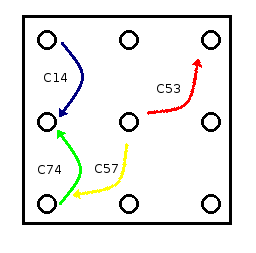
\includegraphics[width=5cm]{gfx/linearBuilder.png}
		 \caption{Estrategia LinearBuilder. Restar azul con verde para transmisión y restar rojo con amarillo para recepción.}
		 \label{fig:linealBuilder}
		\end{figure}

	\item \textbf{CrossBuilder:} Esta estrategia construye ecuaciones utilizando la resta de dos lazos que tengan un elemento en 
		común, llamado central. Dicho elemento puede ser utilizado para transmitir o recibir como en el LinearBuilder. La única 
        diferencia es que en vez de requerir que los tres elementos estén alineados, tienen que formar una L. En otras palabras,
        las rectas de unión deben ser perpendiculares entre sí.
		
        Para ejemplificar, en la figura \ref{fig:crossBuilder} se pueden observar dos pares de lazos de calibración. Si se resta el
        azul con el verde, aprovechando que $C_{12} = C_{14}$, se obtiene una ecuación de la rama de recepción. En cambio, 
        si se resta el rojo con el amarillo, aprovechando que $C_{53} = C_{59}$, se obtiene una ecuación de la rama de 
        transmisión de la antena.

		\begin{figure}[H]
		 \centering
		 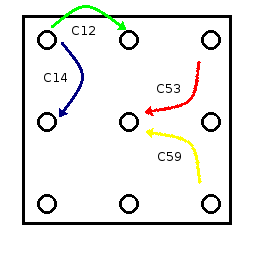
\includegraphics[width=5cm]{gfx/crossBuilder.png}
		 \caption{Estrategia CrossBuilder.}
		 \label{fig:crossBuilder}
		\end{figure}

	\item \textbf{TinyBuilder:} Esta estrategia construye ecuaciones solamente si la cantidad de elementos en alguna dirección, 
        horizontal o vertical, es igual a dos. Utilizando los cuatro lazos de calibración posibles por cada par de elementos 
		que hay en la dirección previamente mencionada, resta los lazos transmitidos por un elemento con los del otro. El resultado 
		es la resta de las dos ramas de transmisión. Para obtener ecuaciones de la diferencia en recepción el razonamiento es 
		análogo, se deben restar los lazos recibidos de uno con los del otro elemento.

        Para ejemplificar, la figura \ref{fig:tinyBuilder} muestra una antena de dos elementos en configuración vertical. En 
        esta estrategia se restan los caminos azules con los verdes aprovechando que $C_{11} = C_{22}$ y que $C_{12} = C_{21}$.
		
		\begin{figure}[H]
		 \centering
		 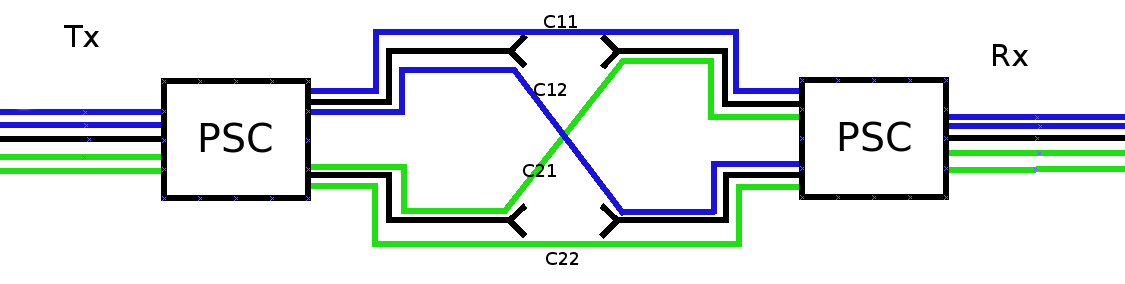
\includegraphics[width=10cm]{gfx/tinyBuilder.png}
		 \caption{Estrategia TinyBuilder.}
		 \label{fig:tinyBuilder}
		\end{figure}

        Nota: En la figura \ref{fig:tinyBuilder} se puede llegar a la interpretación que hay 4 elementos radiantes en vez 
        de 2. Cada elemento fue duplicado para enfatizar que la polarización de transmisión es diferente a la de recepción.

	\item \textbf{DoubleBuilder:} Esta estrategia construye ecuaciones solamente si la cantidad de elementos radiantes de la 
        antena, en cualquiera de sus direcciones, es distinta de dos. A diferencia de la estrategia TinyBuilder, también se 
        utilizan las ramas de recepción de elementos que tengan las mismas distancias a los elementos transmisores.
        
        Para ejemplificar, se tiene una antena de 5 elementos en configuración vertical, como se muestra en la figura 
		\ref{fig:doubleBuilder}. Esta estrategia resta los caminos azules con los verdes aprovechando que $C_{12} = C_{54}$ y que
		$C_{14} = C_{52}$ (por simetría de la antena), dando como resultado dos veces la resta de las ramas de transmisión.
		
		\begin{figure}[H]
		 \centering
		 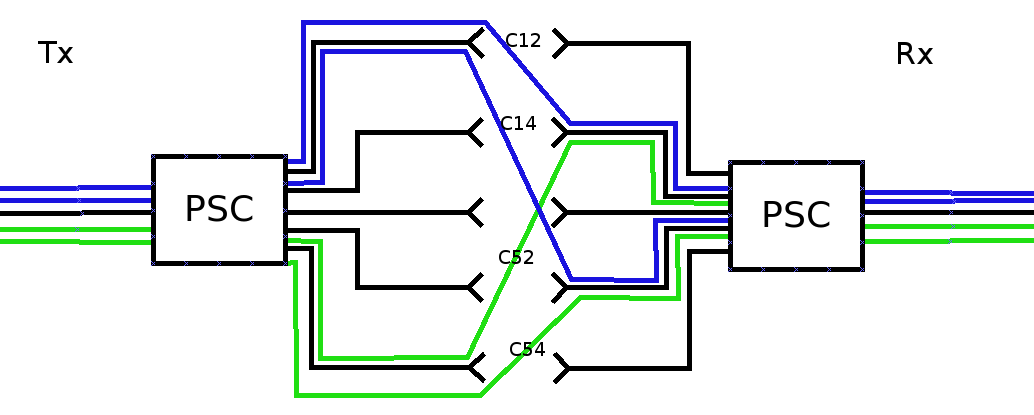
\includegraphics[width=10cm]{gfx/doubleBuilder.png}
		 \caption{Estrategia DoubleBuilder. Al restar los lazos azules con los verdes queda solo la resta de la cadena en 
         transmisión.}
		 \label{fig:doubleBuilder}
		\end{figure}

        Nota: En la figura \ref{fig:doubleBuilder} se puede llegar a la interpretación que hay 10 módulos radiantes en vez 
        de 5. Cada elemento fue duplicado para enfatizar que la polarización de transmisión es diferente a la de recepción.

	\item \textbf{DefaultBuilder:} Esta estrategia se la utiliza para agregar las ecuaciones donde se mide la potencia 
		transmitida/recibida para que el resultado del método sea único. Por ejemplo, puede ser el resultado de la medición de un 
		TRM obtenido de la calibración clásica.
\end{itemize}


Una vez obtenidas todas las ecuaciones de las calibraciones, se procede a utilizar el método de cuadrados mínimos definido en 
la sección \ref{sec:meanSquare}. Para la fase, hay que tener extremo cuidado por su naturaleza modular, por lo tanto, 
previamente a la realización del cálculo de cuadrados mínimos, se acomoda el conjunto de resultados de acuerdo a la sección 
\ref{ssc:mutualPhase}.

\subsection{Configuraciones del sistema}

A modo de resumen, se lista en la tabla \ref{tab:conf_modelo_antena} todas las posibles configuraciones en el modelo para 
realizar los distintos ensayos.

\begin{center}
  \footnotesize
  \centering
  \begin{longtable}{|c|p{9cm}|}
    \hline 
	\multicolumn{2}{|c|}{\textbf{Parámetros de entrada}} \\ 
	\hline
    Frequencia		& Es la frecuenia central de trabajo en Hz \tabularnewline \hline 
    Potencia		& Potencia con la que se alimenta la antena en db \tabularnewline \hline 
    Fase			& Fase con la que se alimenta la antena en grados \tabularnewline \hline 
    Row Steering	& Apuntamiento horizontal que se le quiere dar a la señal transmitida, en grados  \tabularnewline \hline 
    Column Steering	& Apuntamiento vertical que se le quiere dar a la señal transmitida, en grados  \tabularnewline \hline 
	\multicolumn{2}{|c|}{\textbf{Parámetros de calibración}} \\ 
	\hline
	potencia Tx deseada	& Potencia de transmisión deseada para calibrar  \tabularnewline \hline 
	potencia Rx deseada	& Potencia de recepción deseada para calibrar  \tabularnewline \hline 
	Errores	& Son los errores referentes a la hora de calibrar el modelo de antena. Pueden ser: interPulseGainChirpError, 
	interPulsePhaseChirpError, gainChirpRepError, phaseChirpRepError, WalPhaseErrors  \tabularnewline \hline
	\multicolumn{2}{|c|}{\textbf{Parámetros de Antena}} \\ 
	\hline
	Cantidad Filas	& Da la cantidad de módulos radiantes en dirección vertical \tabularnewline \hline 
	Cantidad Columnas	& Da la cantidad de módulos radiantes en dirección horizontal \tabularnewline \hline 
	Separación vertical & Es la separación vertical entre RMs \tabularnewline \hline 
	Separación horizontal & Es la separación horizontal entre RMs \tabularnewline \hline 
	Secuencia de componentes & Es la secuencia de componentes que conforma la RFDN, los mismos pueden ser: cables, psc, trm, circulador, rm \tabularnewline \hline 
	Errores  & Son los componentes de la antena que pueden tener errores. Los mismos pueden ser: RMError, TRMError, CirculatorError, PSCError \tabularnewline \hline 
	TRMs muertos & Es una lista que indica que trms están muertos en el panel de la antena. \tabularnewline \hline 
	\multicolumn{2}{|c|}{\textbf{Componentes de Antena}} \\
	\hline
	$cable_i$ & Se pueden definir tantos cables como se deseen, los parámetros a definir son: attenuation [db], length [m], type = cable \tabularnewline \hline 
	$trm_i$ & Se pueden definir tantos TRMs como se deseen, los parámetros a definir son: gain [db], phaseShift [deg], type = TRM \tabularnewline \hline 
	$psc_{1j}$ & Se pueden definir tantos PSC como se deseen, los parámetros a definir son: outputPorts = $j$, type = PSC1$j$ \tabularnewline \hline 
	circulator & aca se puede definir un circulador, el parámetro a definir es: type = circulator \tabularnewline \hline 
	$rm$ & Se puede definir un RM, el parámetro a definir es: type = RM \tabularnewline \hline 
	\multicolumn{2}{|c|}{\textbf{Desvío estandard del error}} \\
	\hline
	Error del cable & Desvío estándar de los cables. \tabularnewline \hline 
	Error del circulador & Desvío estándar de los circuladores. \tabularnewline \hline 
	Error del TRM & Desvío estándar de los TRMs. \tabularnewline \hline 
	Error del PSC & Desvío estándar de los PSC. \tabularnewline \hline 
	Error del RM & Desvío estándar de los RM. \tabularnewline \hline 
	Error de ganancia entre pulsos & Desvío estándar de ganancia entre pulsos de calibración. \tabularnewline \hline 
	Error de fase entre pulsos & Desvío estándar de fase entre pulsos de calibración. \tabularnewline \hline 
	Error de ganancia de la chirp replica & Desvío estándar de ganancia de la chirp replica. \tabularnewline \hline 
	Error de fase de la chirp replica & Desvío estándar de fase de la chirp replica. \tabularnewline \hline 
	Error de fase del walsh & Desvío estándar de fase del seteo de los defasadores en calibración. \tabularnewline \hline 
	\caption{Configuraciones del modelo de antena}
  \end{longtable}
  \label{tab:conf_modelo_antena}
\end{center}

A su vez, también se puede configurar que tipo de calibración se desea correr para poder obtener los resultados y se pueden 
graficar tanto los diagramas de radiación obtenidos en algún corte en azimuth/rango o el conjunto de ganancias y fases con 
respecto al valor ideal. La figura \ref{fig:visualPackage} muestra el diagrama de clases del visualizador.

\begin{figure}[H]
 \centering
 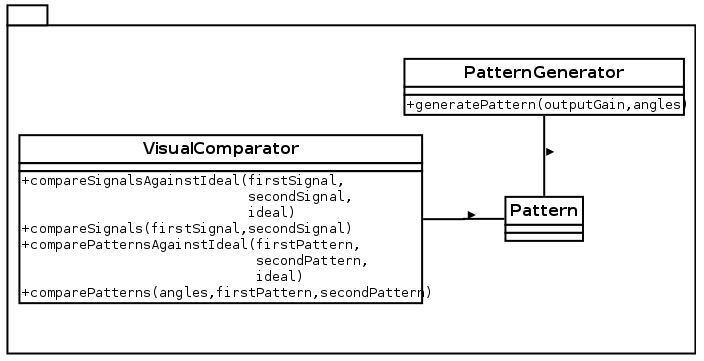
\includegraphics[width=11cm]{gfx/visualPackage.png}
 \caption{Diagrama de clases de los visualizadores.}
 \label{fig:visualPackage}
\end{figure}


%\chapter{Simulaciones}
\lhead{\emph{Simulaciones}}

En este capítulo se presentan las mediciones y ensayos realizados para estudiar y comparar como se comportan ambos métodos de
calibración: clásica y utilizando acoplamientos mutuos.

La configuración de la antena a utilizar para todos los ensayos está especificada en la tabla \ref{tab:configurationUsed} y 
consta de 70 elementos radiantes. Las especificaciones de las propiedades físicas de cada componente están definidas en la 
tabla \ref{tab:configurationOfComponents}.
\begin{table}[H]
  \footnotesize
  \centering
  \begin{tabular}{|c|c|}
	\hline
	\textbf{Componente de Antena} & \textbf{Configuración} \tabularnewline \hline 
	freq &  1275000000 [Hz] \tabularnewline\hline 
	power & 0 [dB] \tabularnewline \hline 
	phase & 0 [deg] \tabularnewline \hline 
	desiredTxPower & 6 [dB] \tabularnewline \hline 
	desiredRxPower & 0 [dB] \tabularnewline \hline 
	quantityRows & 7 \tabularnewline \hline 
	quantityColumns & 10 \tabularnewline \hline 
	verticalSeparation & 0.2 [m] \tabularnewline \hline 
	hotizontalSeparation & 0.2 [m] \tabularnewline \hline 
	componentSequence & [cable1, psc17, cable1, psc15, cable2, psc12, trm, circulator, cable3, rm] \tabularnewline \hline 
  \end{tabular}
  \caption{Configuración de la antena común para todos los ensayos.}
  \label{tab:configurationUsed}
\end{table}
\begin{table}[H]
  \footnotesize
  \centering
  \begin{tabular}{|c|c|c|}
	\hline
	\textbf{Componente de Antena} & \textbf{Cacarcterísticas físicas} & \textbf{Configuración} \tabularnewline \hline 
	\multirow{2}{*}{cable1} &  attenuation [db] & 0.1\tabularnewline \cline{2-3}
	 & length [m] & 0.45\tabularnewline \hline 
	\multirow{2}{*}{cable2} &  attenuation [db] & 0.1\tabularnewline \cline{2-3}
	 & length [m] & 8\tabularnewline \hline 
	\multirow{2}{*}{cable3} &  attenuation [db] & 0.1\tabularnewline \cline{2-3}
	 & length [m] & 0.5\tabularnewline \hline 
	psc17 & outputPorts & 7\tabularnewline \hline
	psc15 & outputPorts & 5\tabularnewline \hline
	psc12 & outputPorts & 2\tabularnewline \hline
	\multirow{2}{*}{TRM} & gain [db] & 10\tabularnewline \cline{2-3}
	 & phaseShift [deg] & 10\tabularnewline \hline 
	circulator & & \tabularnewline \hline 
	RM & & \tabularnewline \hline 
  \end{tabular}
  \caption{Configuración de las propiedades físicas de cada componente de la antena utilizada en todos los ensayos.}
  \label{tab:configurationOfComponents}
\end{table}
La numeración de los elementos tiene un orden de izquierda a derecha y de arriba hacia abajo, de tal forma que el elemnto cero 
es el superior izquierdo de la antena.

\begin{figure}[H]
 \centering
 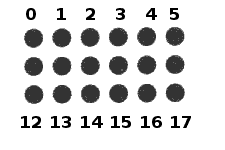
\includegraphics[width=8cm]{gfx/arrayNumeration.png}
 \caption{Numeración de los elementos de un panel de antena.}
 \label{fig:arrayNumeration}
\end{figure}

Para una mayor claridad, todos los gráficos representan cómo ambos métodos calibran la antena en un estado puntual.

Todos los ensayos de las siguientes secciones poseen las siguientes característicias:
\begin{itemize}
	\item Se utilizan diferentes apuntamientos de la antena. Los cuales son uniforme, 10 grados en la dirección horizontal y 10 
		grados en la dirección vertical.
	\item Se muestra un gráfico de la potencia y fase transmitida para cada apuntamiento utilizado. En los cuales se observan las
		señales sin calibrar, calibrada e ideal. 
	\item Se grafican los diagramas de antena para los cortes horizontal y vertical de las señales transmitidas sin calibrar, 
		calibradas e ideales.
\end{itemize}


\section{Sin dispersiones}

Los ensayos de esta sección tienen las siguientes caracterísiticas,
\begin{itemize}
	\item Los componentes de antena no tienen ningún problema de funcionamiento ni hay desadaptaciones.
	\item No hay dispersiones de calibración.
	\item No hay dispersiones en la señal.
\end{itemize}

\subsection{Utilizando la calibración clásica}

En las figuras \ref{fig:nonErrClassical0deg}, \ref{fig:nonErrClassical10degCol} y \ref{fig:nonErrClassical10degRow} se muestran
los resultados de la calibración clásica con una antena sin dispersiones. Se puede apreciar que, si bien la antena tiene un 
comportamiento ideal, las mediciones no son completamente correctas. Dicho desvío se debe a que el método no abarca la 
totalidad de la antena.


\subsubsection{Apuntamiento uniforme}

Los gráficos de la figura \ref{fig:nonErrClassical0deg} muestran que el calibrador, por no abarcar la totalidad del sistema, no 
puede determinar correctamente ni la ganancia ni fase de la antena. Pero, como dicho desvío es el mismo para todos los elementos,
el diagrama resultante mantiene su forma y sus atributos no se modifican, salvo la ganancia total.

La tabla \ref{tab:nonErrClassical0deg} muestra como la ganancia relativa de los lóbulos secundarios con respecto al del lóbulo
principal de cada diagrama se mantienen invariantes e iguales al del diagrama ideal. A su vez se puede observar como la diferencia
de la ganancia del diagrama calibrado disminuye pero no llega a ser igual a cero.
\begin{figure}[H]
	\centering
 	\subfloat[]{
		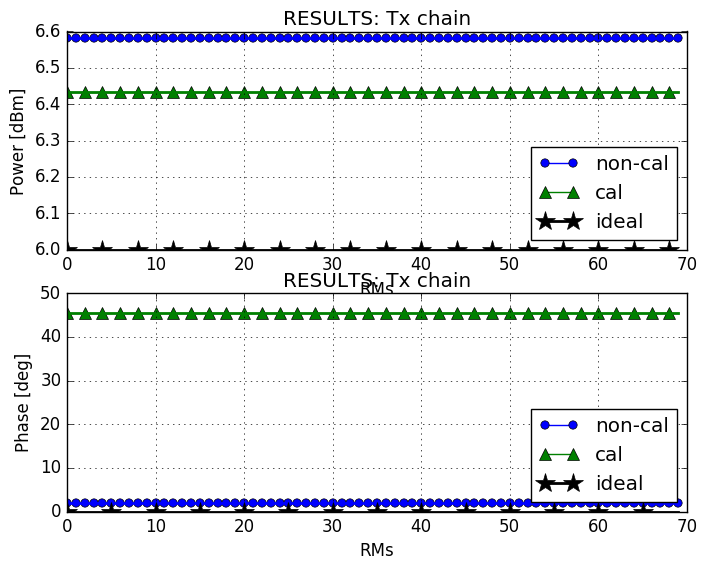
\includegraphics[width=9cm]{gfx/nonErrClassical0deg.png}}

	\subfloat[]{
		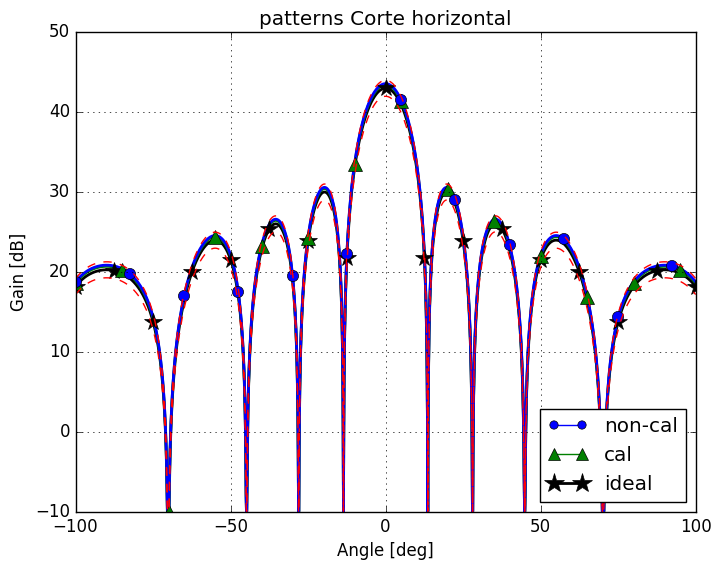
\includegraphics[width=7cm]{gfx/nonErrClassical0degAzCut.png}}
 	\subfloat[]{
		\includegraphics[width=7cm]{gfx/nonErrClassical0degElCut.png}}
	\caption{Señal transmitida utilizando calibración clásica. (a) ganancia y fase transmitida. (b) corte horizontal del 
	diagrama de radiación y (c) corte vertical del diagrama de radiación.}
	\label{fig:nonErrClassical0deg}
\end{figure}
\begin{table}[H]
  \footnotesize
  \centering
  \begin{tabular}{|c|c|p{2cm}|p{2.5cm}|p{2.5cm}|p{2.5cm}|}
    \cline{2-6}
    \multicolumn{1}{c|}{} & Corte & Ganancia - lóbulo izq. [dBc] & Ganancia - lóbulo central [dB] &
    Ganancia - lóbulo der. [dBc] & Ancho - lóbulo central -3dB \tabularnewline\hline
    \multirow{2}{2cm}{Pat. sin calibrar} & H & 12.97 & 43.48 & 12.97 & 12.0 \tabularnewline\cline{2-6}
     & V & 12.65 & 43.48 & 12.65 & 17.4 \tabularnewline\hline
    \multirow{2}{2cm}{Pat. calibrado} & H & 12.97 & 43.34 & 12.97 & 12.0 \tabularnewline\cline{2-6}
     & V & 12.65 & 43.34 & 12.65 & 17.4 \tabularnewline\hline
    \multirow{2}{2cm}{Pat. ideal} & H & 12.97 & 42.9 & 12.97 & 12.0 \tabularnewline\cline{2-6}
     & V & 12.65 & 42.9 & 12.65 & 17.4 \tabularnewline\hline
    \multirow{2}{2cm}{Dif. sin calibrar} & H & 0.0 & 0.58 & 0.0 & 0.0\tabularnewline\cline{2-6}
     & V & 0.0 & 0.58 & 0.0 & 0.0 \tabularnewline\hline
    \multirow{2}{2cm}{Dif. calibrado} & H & 0.0 & 0.44 & 0.0 & 0.0 \tabularnewline\cline{2-6}
     & V & 0.0 & 0.44 & 0.0 & 0.0 \tabularnewline\hline
  \end{tabular}
  \caption{Propiedades de los diagramas de radiación calibrados y sin calibrar comparados con el ideal.}
  \label{tab:nonErrClassical0deg}
\end{table}

\subsubsection{Apuntamiento 10 grados en dirección horizontal}

Los gráficos de la figura \ref{fig:nonErrClassical10degCol} muestran que el calibrador, por no abarcar la totalidad del sistema,
no puede determinar correctamente ni la ganancia ni fase de la antena. Pero, como dicho desvío es el mismo para todos los elementos,
el diagrama resultante mantiene su forma y sus atributos no se modifican, salvo la ganancia total.

\begin{figure}[H]
	\centering
 	\subfloat[]{
		\includegraphics[width=9cm]{gfx/nonErrClassical10degCol.png}}

	\subfloat[]{
		\includegraphics[width=7cm]{gfx/nonErrClassical10degColAzCut.png}}
 	\subfloat[]{
		\includegraphics[width=7cm]{gfx/nonErrClassical10degColElCut.png}}
	\caption{Señal transmitida utilizando calibración clásica. (a) ganancia y fase transmitida. (b) corte horizontal del 
	diagrama de radiación y (c) corte vertical del diagrama de radiación.}
	\label{fig:nonErrClassical10degCol}
\end{figure}

La tabla \ref{tab:nonErrClassical0deg} muestra como la ganancia relativa de los lóbulos secundarios con respecto al del lóbulo
principal de cada diagrama se mantienen invariantes e iguales al del diagrama ideal. A su vez se puede observar como la diferencia
de la ganancia del diagrama calibrado disminuye pero no llega a ser igual a cero.
\begin{table}[H]
  \footnotesize
  \centering
  \begin{tabular}{|c|c|p{2cm}|p{2.5cm}|p{2.5cm}|p{2.5cm}|}
    \cline{2-6}
    \multicolumn{1}{c|}{} & Corte & Ganancia - lóbulo izq. [dBc] & Ganancia - lóbulo central [dB] &
    Ganancia - lóbulo der. [dBc] & Ancho - lóbulo central -3dB \tabularnewline\hline
    \multirow{2}{2cm}{Pat. sin calibrar} & H & 12.97 & 43.48 & 12.97 & 12.4 \tabularnewline\cline{2-6}
     & V & 12.65 & 33.54 & 12.65 & 17.4 \tabularnewline\hline
    \multirow{2}{2cm}{Pat. calibrado} & H & 12.97 & 43.34 & 12.97 & 12.4 \tabularnewline\cline{2-6}
     & V & 12.65 & 33.4 & 12.65 & 17.4 \tabularnewline\hline
    \multirow{2}{2cm}{Pat. ideal} & H & 12.97 & 42.9 & 12.97 & 12.4 \tabularnewline\cline{2-6}
     & V & 12.65 & 32.96 & 12.65 & 17.4 \tabularnewline\hline
    \multirow{2}{2cm}{Dif. sin calibrar} & H & 0.0 & 0.58 & 0.0 & 0.0\tabularnewline\cline{2-6}
     & V & 0.0 & 0.58 & 0.0 & 0.0 \tabularnewline\hline
    \multirow{2}{2cm}{Dif. calibrado} & H & 0.0 & 0.44 & 0.0 & 0.0 \tabularnewline\cline{2-6}
     & V & 0.0 & 0.44 & 0.0 & 0.0 \tabularnewline\hline
  \end{tabular}
  \caption{Propiedades de los diagramas de radiación calibrados y sin calibrar comparados con el ideal.}
  \label{tab:nonErrClassical10degCol}
\end{table}


\subsubsection{Apuntamiento 10 grados en dirección vertical}

Los gráficos de la figura \ref{fig:nonErrClassical10degRow} muestran que el calibrador, por no abarcar la totalidad del sistema,
no puede determinar correctamente ni la ganancia ni fase de la antena. Pero, como dicho desvío es el mismo para todos los elementos,
el diagrama resultante mantiene su forma y sus atributos no se modifican, salvo la ganancia total.

La tabla \ref{tab:nonErrClassical0deg} muestra como la ganancia relativa de los lóbulos secundarios con respecto al del lóbulo
principal de cada diagrama se mantienen invariantes e iguales al del diagrama ideal. A su vez se puede observar como la diferencia
de la ganancia del diagrama calibrado disminuye pero no llega a ser igual a cero.

\begin{figure}[H]
	\centering
 	\subfloat[]{
		\includegraphics[width=9cm]{gfx/nonErrClassical10degRow.png}}

	\subfloat[]{
		\includegraphics[width=7cm]{gfx/nonErrClassical10degRowAzCut.png}}
 	\subfloat[]{
		\includegraphics[width=7cm]{gfx/nonErrClassical10degRowElCut.png}}
	\caption{Señal transmitida utilizando calibración clásica. (a) ganancia y fase transmitida. (b) corte horizontal del 
	diagrama de radiación y (c) corte vertical del diagrama de radiación.}
	\label{fig:nonErrClassical10degRow}
\end{figure}
\begin{table}[H]
  \footnotesize
  \centering
  \begin{tabular}{|c|c|p{2cm}|p{2.5cm}|p{2.5cm}|p{2.5cm}|}
    \cline{2-6}
    \multicolumn{1}{c|}{} & Corte & Ganancia - lóbulo izq. [dBc] & Ganancia - lóbulo central [dB] &
    Ganancia - lóbulo der. [dBc] & Ancho - lóbulo central -3dB \tabularnewline\hline
    \multirow{2}{2cm}{Pat. sin calibrar} & H & 12.97 & 39.34 & 12.97 & 12.0 \tabularnewline\cline{2-6}
     & V & 12.65 & 43.48 & 12.65 & 17.8 \tabularnewline\hline
    \multirow{2}{2cm}{Pat. calibrado} & H & 12.97 & 39.19 & 12.97 & 12.0 \tabularnewline\cline{2-6}
     & V & 12.65 & 43.34 & 12.65 & 17.8 \tabularnewline\hline
    \multirow{2}{2cm}{Pat. ideal} & H & 12.97 & 38.76 & 12.97 & 12.0 \tabularnewline\cline{2-6}
     & V & 12.65 & 42.9 & 12.65 & 17.8 \tabularnewline\hline
    \multirow{2}{2cm}{Dif. sin calibrar} & H & 0.0 & 0.58 & 0.0 & 0.0\tabularnewline\cline{2-6}
     & V & 0.0 & 0.58 & 0.0 & 0.0 \tabularnewline\hline
    \multirow{2}{2cm}{Dif. calibrado} & H & 0.0 & 0.43 & 0.0 & 0.0 \tabularnewline\cline{2-6}
     & V & 0.0 & 0.44 & 0.0 & 0.0 \tabularnewline\hline
  \end{tabular}
  \caption{Propiedades de los diagramas de radiación calibrados y sin calibrar comparados con el ideal.}
  \label{tab:nonErrClassical10degRow}
\end{table}


\subsection{Utilizando la calibración con acoplamientos mutuos}


\subsubsection{Apuntamiento uniforme}

Los gráficos de la figura \ref{fig:nonErrMutual0deg} muestran que el calibrador funciona correctamente para estimar y corregir la 
fase y ganancia del sistema. Los diagramas de radiación calibrados resultan iguales al ideal.

En la tabla \ref{tab:nonErrMutual0deg} se puede apreciar como todos los parámetros de los diagramas calibrados resultan 
exactamente igual al ideal.

\begin{figure}[H]
	\centering
 	\subfloat[]{
		\includegraphics[width=9cm]{gfx/nonErrMutual0deg.png}}

	\subfloat[]{
		\includegraphics[width=7cm]{gfx/nonErrMutual0degAzCut.png}}
 	\subfloat[]{
		\includegraphics[width=7cm]{gfx/nonErrMutual0degElCut.png}}
	\caption{Señal transmitida calibrada por acoplamientos mutuos. (a) ganancia y fase transmitida. (b) corte horizontal del 
	diagrama de radiación y (c) corte vertical del diagrama de radiación.}
	\label{fig:nonErrMutual0deg}
\end{figure}

\begin{table}[H]
  \footnotesize
  \centering
  \begin{tabular}{|c|c|p{2cm}|p{2.5cm}|p{2.5cm}|p{2.5cm}|}
    \cline{2-6}
    \multicolumn{1}{c|}{} & Corte & Ganancia - lóbulo izq. [dBc] & Ganancia - lóbulo central [dB] &
    Ganancia - lóbulo der. [dBc] & Ancho - lóbulo central -3dB \tabularnewline\hline
    \multirow{2}{2cm}{Pat. sin calibrar} & H & 12.65 & 47.29 & 12.65 & 17.4 \tabularnewline\cline{2-6}
     & V & 13.19 & 47.29 & 13.19 & 6.0 \tabularnewline\hline
    \multirow{2}{2cm}{Pat. calibrado} & H & 12.65 & 48.92 & 12.65 & 17.4 \tabularnewline\cline{2-6}
     & V & 13.19 & 48.92 & 13.19 & 6.0 \tabularnewline\hline
    \multirow{2}{2cm}{Pat. ideal} & H & 12.65 & 48.92 & 12.65 & 17.4 \tabularnewline\cline{2-6}
     & V & 13.19 & 48.92 & 13.19 & 6.0 \tabularnewline\hline
    \multirow{2}{2cm}{Dif. sin calibrar} & H & 0.0 & -1.63 & 0.0 & 0.0\tabularnewline\cline{2-6}
     & V & 0.0 & -1.63 & 0.0 & 0.0 \tabularnewline\hline
    \multirow{2}{2cm}{Dif. calibrado} & H & 0.0 & 0.0 & 0.0 & 0.0 \tabularnewline\cline{2-6}
     & V & 0.0 & 0.0 & 0.0 & 0.0 \tabularnewline\hline
  \end{tabular}
  \caption{Propiedades de los diagramas de radiación calibrados y sin calibrar comparados con el ideal.}
  \label{tab:nonErrMutual0deg}
\end{table}


\subsubsection{Apuntamiento 10 grados en dirección horizontal}

Los gráficos de la figura \ref{fig:nonErrMutual10degCol} muestran que el calibrador funciona correctamente para estimar y 
corregir la fase y ganancia del sistema utilizando un apuntamiento diferente al uniforme logrando así que los diagramas de 
radiación calibrados resultan iguales al ideal. A su vez, se puede apreciar que la fase muestra un diagrama estilo diente 
de sierra porque, al ser un apuntamiento horizontal, la fase entre columnas de la antena es diferente (y la numeración de 
los elementos radiantes es creciente de a filas).

En la tabla \ref{tab:nonErrMutual0deg} se puede apreciar como todos los parámetros de los diagramas calibrados resultan 
exactamente igual al ideal.

\begin{figure}[H]
	\centering
 	\subfloat[]{
		\includegraphics[width=9cm]{gfx/nonErrMutual10degCol.png}}

	\subfloat[]{
		\includegraphics[width=7cm]{gfx/nonErrMutual10degColAzCut.png}}
 	\subfloat[]{
		\includegraphics[width=7cm]{gfx/nonErrMutual10degColElCut.png}}
	\caption{Señal transmitida calibrada por acoplamientos mutuos. (a) ganancia y fase transmitida. (b) corte horizontal del 
	diagrama de radiación y (c) corte vertical del diagrama de radiación.}
	\label{fig:nonErrMutual10degCol}
\end{figure}

\begin{table}[H]
  \footnotesize
  \centering
  \begin{tabular}{|c|c|p{2cm}|p{2.5cm}|p{2.5cm}|p{2.5cm}|}
    \cline{2-6}
    \multicolumn{1}{c|}{} & Corte & Ganancia - lóbulo izq. [dBc] & Ganancia - lóbulo central [dB] &
    Ganancia - lóbulo der. [dBc] & Ancho - lóbulo central -3dB \tabularnewline\hline
    \multirow{2}{2cm}{Pat. sin calibrar} & H & 12.97 & 43.48 & 12.97 & 12.4 \tabularnewline\cline{2-6}
     & V & 12.65 & 33.54 & 12.65 & 17.4 \tabularnewline\hline
    \multirow{2}{2cm}{Pat. calibrado} & H & 12.97 & 42.9 & 12.97 & 12.4 \tabularnewline\cline{2-6}
     & V & 12.65 & 32.96 & 12.65 & 17.4 \tabularnewline\hline
    \multirow{2}{2cm}{Pat. ideal} & H & 12.97 & 42.9 & 12.97 & 12.4 \tabularnewline\cline{2-6}
     & V & 12.65 & 32.96 & 12.65 & 17.4 \tabularnewline\hline
    \multirow{2}{2cm}{Dif. sin calibrar} & H & 0.0 & 0.58 & 0.0 & 0.0\tabularnewline\cline{2-6}
     & V & 0.0 & 0.58 & 0.0 & 0.0 \tabularnewline\hline
    \multirow{2}{2cm}{Dif. calibrado} & H & 0.0 & 0.0 & 0.0 & 0.0 \tabularnewline\cline{2-6}
     & V & 0.0 & 0.0 & 0.0 & 0.0 \tabularnewline\hline
  \end{tabular}
  \caption{Propiedades de los diagramas de radiación calibrados y sin calibrar comparados con el ideal.}
  \label{tab:nonErrMutual10degCol}
\end{table}


\subsubsection{Apuntamiento 10 grados en dirección vertical}

Los gráficos de la figura \ref{fig:nonErrMutual10degRow} muestran que el calibrador funciona correctamente para estimar y 
corregir la fase y ganancia del sistema utilizando un apuntamiento diferente al uniforme logrando así que los diagramas de 
radiación calibrados resultan iguales al ideal. A su vez, se puede apreciar que la fase muestra un diagrama estilo escalonado
porque, al ser un apuntamiento vertical, la fase entre filas de la antena difiere (y la numeración de los elementos radiantes 
es creciente de a filas).

\begin{figure}[H]
	\centering
 	\subfloat[]{
		\includegraphics[width=9cm]{gfx/nonErrMutual10degRow.png}}

	\subfloat[]{
		\includegraphics[width=7cm]{gfx/nonErrMutual10degRowAzCut.png}}
 	\subfloat[]{
		\includegraphics[width=7cm]{gfx/nonErrMutual10degRowElCut.png}}
	\caption{Señal transmitida calibrada por acoplamientos mutuos. (a) ganancia y fase transmitida. (b) corte horizontal del 
	diagrama de radiación y (c) corte vertical del diagrama de radiación.}
	\label{fig:nonErrMutual10degRow}
\end{figure}

En la tabla \ref{tab:nonErrMutual10degRow} se puede apreciar como todos los parámetros de los diagramas calibrados resultan 
exactamente igual al ideal.

\begin{table}[H]
  \footnotesize
  \centering
  \begin{tabular}{|c|c|p{2cm}|p{2.5cm}|p{2.5cm}|p{2.5cm}|}
    \cline{2-6}
    \multicolumn{1}{c|}{} & Corte & Ganancia - lóbulo izq. [dBc] & Ganancia - lóbulo central [dB] &
    Ganancia - lóbulo der. [dBc] & Ancho - lóbulo central -3dB \tabularnewline\hline
    \multirow{2}{2cm}{Pat. sin calibrar} & H & 12.97 & 28.29 & 12.97 & 12.0 \tabularnewline\cline{2-6}
     & V & 13.22 & 50.15 & 13.22 & 5.0 \tabularnewline\hline
    \multirow{2}{2cm}{Pat. calibrado} & H & 12.97 & 32.1 & 12.97 & 12.0 \tabularnewline\cline{2-6}
     & V & 13.22 & 53.96 & 13.22 & 5.0 \tabularnewline\hline
    \multirow{2}{2cm}{Pat. ideal} & H & 12.97 & 32.1 & 12.97 & 12.0 \tabularnewline\cline{2-6}
     & V & 13.22 & 53.96 & 13.22 & 5.0 \tabularnewline\hline
    \multirow{2}{2cm}{Dif. sin calibrar} & H & 0.0 & -3.81 & 0.0 & 0.0\tabularnewline\cline{2-6}
     & V & 0.0 & -3.81 & 0.0 & 0.0 \tabularnewline\hline
    \multirow{2}{2cm}{Dif. calibrado} & H & 0.0 & 0.0 & 0.0 & 0.0 \tabularnewline\cline{2-6}
     & V & 0.0 & 0.0 & 0.0 & 0.0 \tabularnewline\hline
  \end{tabular}
  \caption{Propiedades de los diagramas de radiación calibrados y sin calibrar comparados con el ideal.}
  \label{tab:nonErrMutual10degRow}
\end{table}


\section{Rotura de varios TRMs}
Los ensayos de esta sección tienen las siguientes caracterísiticas,
\begin{itemize}
	\item Salvo tres TRMs que están rotos, el resto de los componentes de antena no tienen ningún prolema de funcionamiento ni 
		desadaptaciones. Las posiciones de los TRMs son: [1,0], [3,4] y [5,5]. La nomenclatura de lectura es [fila, columna] con 
		valores desde 0.
	\item No hay errores de calibración.
	\item No hay errores en la señal.
\end{itemize}

\subsection{Utilizando la calibración clásica}
En las figuras \ref{fig:deadTRMsClassical0deg}, \ref{fig:deadTRMsClassical10degCol} y \ref{fig:deadTRMsClassical10degRow} se 
muestran los resultados de la calibración clásica para una antena con algunos TRMs destruidos. Se puede apreciar que no hay 
modificaciones en el comportamiento del método al calibrar el resto de los elementos y que el diagrama se deforma de una manera 
significativa.

\subsubsection{Apuntamiento uniforme}

Los gráficos de la figura \ref{fig:deadTRMsClassical0deg} muestran que el calibrador, dejando de lado la diferencia de 
estimación tanto de fase como ganancia por no abarcar la totalidad del sistema, funciona correctamente. Los elementos 10, 34 y 
55 presentan una ganancia que equivaldría al piso de ruido.

A causa de los TRMs muertos, se aprecia un aumento considerable de ambos lóbulos secundarios del corte horizontal. El corte 
vertical no presenta grandes desvíos.

\begin{figure}[H]
	\centering
 	\subfloat[]{
		\includegraphics[width=9cm]{gfx/deadTRMsClassical0deg.png}}

	\subfloat[]{
		\includegraphics[width=7cm]{gfx/deadTRMsClassical0degAzCut.png}}
 	\subfloat[]{
		\includegraphics[width=7cm]{gfx/deadTRMsClassical0degElCut.png}}
	\caption{Señal transmitida utilizando calibración clásica. (a) ganancia y fase transmitida. (b) corte horizontal del 
	diagrama de radiación y (c) corte vertical del diagrama de radiación.}
	\label{fig:deadTRMsClassical0deg}
\end{figure}

La tabla \ref{tab:deadTRMsClassical0deg} muestra que las diferencias de ganancia de los lóbulos secundarios entre los diagramas 
reales y el ideal para el corte horizontal es del orden del dB y  este es el valor límite admisible. En el corte vertical dicha 
diferencia es mucho menor.

\begin{table}[H]
  \footnotesize
  \centering
  \begin{tabular}{|c|c|p{2cm}|p{2.5cm}|p{2.5cm}|p{2.5cm}|}
    \cline{2-6}
    \multicolumn{1}{c|}{} & Corte & Ganancia - lóbulo izq. [dBc] & Ganancia - lóbulo central [dB] &
    Ganancia - lóbulo der. [dBc] & Ancho - lóbulo central -3dB \tabularnewline\hline
    \multirow{2}{2cm}{Pat. sin calibrar} & H & 11.93 & 43.1 & 11.93 & 12.0 \tabularnewline\cline{2-6}
     & V & 12.65 & 43.1 & 12.65 & 17.2 \tabularnewline\hline
    \multirow{2}{2cm}{Pat. calibrado} & H & 11.93 & 42.96 & 11.93 & 12.0 \tabularnewline\cline{2-6}
     & V & 12.65 & 42.96 & 12.65 & 17.2 \tabularnewline\hline
    \multirow{2}{2cm}{Pat. ideal} & H & 12.97 & 42.9 & 12.97 & 12.0 \tabularnewline\cline{2-6}
     & V & 12.65 & 42.9 & 12.65 & 17.4 \tabularnewline\hline
    \multirow{2}{2cm}{Dif. sin calibrar} & H & -1.04 & 0.2 & -1.04 & 0.0\tabularnewline\cline{2-6}
     & V & 0.0 & 0.2 & 0.0 & -0.2 \tabularnewline\hline
    \multirow{2}{2cm}{Dif. calibrado} & H & -1.04 & 0.06 & -1.04 & 0.0 \tabularnewline\cline{2-6}
     & V & 0.0 & 0.06 & 0.0 & -0.2 \tabularnewline\hline
  \end{tabular}
  \caption{Propiedades de los diagramas de radiación calibrados y sin calibrar comparados con el ideal.}
  \label{tab:deadTRMsClassical0deg}
\end{table}


\subsubsection{Apuntamiento 10 grados en dirección horizontal}

Los gráficos de la figura \ref{fig:deadTRMsClassical10degCol} muestran que el calibrador, dejando de lado la diferencia de 
estimación tanto de fase como ganancia por no abarcar la totalidad del sistema, funciona correctamente. Los elementos 10, 34 y 
55 presentan una ganancia que equivaldría al piso de ruido.

A causa de los TRMs muertos, se aprecia un aumento considerable de ambos lóbulos secundarios de los cortes horizontal y vertical.

La tabla \ref{tab:deadTRMsClassical10degCol} muestra que las diferencias de ganancia de los lóbulos secundarios entre los 
diagramas de radiación reales y el ideal para el corte horizontal es del orden del dB y para el vertical los dos dBs. Estas 
diferencias ya son mayores a las permitidas por la máscara.

\begin{figure}[H]
	\centering
 	\subfloat[]{
		\includegraphics[width=9cm]{gfx/deadTRMsClassical10degCol.png}}

	\subfloat[]{
		\includegraphics[width=7cm]{gfx/deadTRMsClassical10degColAzCut.png}}
 	\subfloat[]{
		\includegraphics[width=7cm]{gfx/deadTRMsClassical10degColElCut.png}}
	\caption{Señal transmitida utilizando calibración clásica. (a) ganancia y fase transmitida. (b) corte horizontal del 
	diagrama de radiación y (c) corte vertical del diagrama de radiación.}
	\label{fig:deadTRMsClassical10degCol}
\end{figure}
\begin{table}[H]
  \footnotesize
  \centering
  \begin{tabular}{|c|c|p{2cm}|p{2.5cm}|p{2.5cm}|p{2.5cm}|}
    \cline{2-6}
    \multicolumn{1}{c|}{} & Corte & Ganancia - lóbulo izq. [dBc] & Ganancia - lóbulo central [dB] &
    Ganancia - lóbulo der. [dBc] & Ancho - lóbulo central -3dB \tabularnewline\hline
    \multirow{2}{2cm}{Pat. sin calibrar} & H & 11.93 & 43.1 & 11.94 & 12.4 \tabularnewline\cline{2-6}
     & V & 11.91 & 32.98 & 10.26 & 16.8 \tabularnewline\hline
    \multirow{2}{2cm}{Pat. calibrado} & H & 11.93 & 42.96 & 11.94 & 12.4 \tabularnewline\cline{2-6}
     & V & 11.91 & 32.83 & 10.26 & 16.8 \tabularnewline\hline
    \multirow{2}{2cm}{Pat. ideal} & H & 12.97 & 42.9 & 12.97 & 12.4 \tabularnewline\cline{2-6}
     & V & 12.65 & 32.96 & 12.65 & 17.4 \tabularnewline\hline
    \multirow{2}{2cm}{Dif. sin calibrar} & H & -1.04 & 0.2 & -1.03 & 0.0\tabularnewline\cline{2-6}
     & V & -0.74 & 0.02 & -2.39 & -0.6 \tabularnewline\hline
    \multirow{2}{2cm}{Dif. calibrado} & H & -1.04 & 0.06 & -1.03 & 0.0 \tabularnewline\cline{2-6}
     & V & -0.74 & -0.13 & -2.39 & -0.6 \tabularnewline\hline
  \end{tabular}
  \caption{Propiedades de los diagramas de radiación calibrados y sin calibrar comparados con el ideal.}
  \label{tab:deadTRMsClassical10degCol}
\end{table}


\subsubsection{Apuntamiento 10 grados en dirección vertical}

Los gráficos de la figura \ref{fig:deadTRMsClassical10degRow} muestran que el calibrador, dejando de lado la diferencia de 
estimación tanto de fase como ganancia por no abarcar la totalidad del sistema, funciona correctamente. Los elementos 10, 34 y 
55 presentan una ganancia que equivaldría al piso de ruido.

A causa de los TRMs muertos, se aprecia un aumento considerable de ambos lóbulos secundarios de los cortes horizontal y vertical.

\begin{figure}[H]
	\centering
 	\subfloat[]{
		\includegraphics[width=9cm]{gfx/deadTRMsClassical10degRow.png}}

	\subfloat[]{
		\includegraphics[width=7cm]{gfx/deadTRMsClassical10degRowAzCut.png}}
 	\subfloat[]{
		\includegraphics[width=7cm]{gfx/deadTRMsClassical10degRowElCut.png}}
	\caption{Señal transmitida utilizando calibración clásica. (a) ganancia y fase transmitida. (b) corte horizontal del 
	diagrama de radiación y (c) corte vertical del diagrama de radiación.}
	\label{fig:deadTRMsClassical10degRow}
\end{figure}

La tabla \ref{tab:deadTRMsClassical10degRow} muestra que las diferencias de ganancia de los lóbulos secundarios entre los 
diagramas de radiación reales y el ideal para el corte horizontal supera el dB y para el vertical no se aprecian diferencias. 
Estas diferencias ya son mayores a las permitidas por la máscara.

\begin{table}[H]
  \footnotesize
  \centering
  \begin{tabular}{|c|c|p{2cm}|p{2.5cm}|p{2.5cm}|p{2.5cm}|}
    \cline{2-6}
    \multicolumn{1}{c|}{} & Corte & Ganancia - lóbulo izq. [dBc] & Ganancia - lóbulo central [dB] &
    Ganancia - lóbulo der. [dBc] & Ancho - lóbulo central -3dB \tabularnewline\hline
    \multirow{2}{2cm}{Pat. sin calibrar} & H & 11.29 & 38.89 & 11.81 & 12.0 \tabularnewline\cline{2-6}
     & V & 12.65 & 43.1 & 12.65 & 17.8 \tabularnewline\hline
    \multirow{2}{2cm}{Pat. calibrado} & H & 11.29 & 38.74 & 11.81 & 12.0 \tabularnewline\cline{2-6}
     & V & 12.65 & 42.96 & 12.65 & 17.8 \tabularnewline\hline
    \multirow{2}{2cm}{Pat. ideal} & H & 12.97 & 38.76 & 12.97 & 12.0 \tabularnewline\cline{2-6}
     & V & 12.65 & 42.9 & 12.65 & 17.8 \tabularnewline\hline
    \multirow{2}{2cm}{Dif. sin calibrar} & H & -1.68 & 0.13 & -1.16 & 0.0\tabularnewline\cline{2-6}
     & V & 0.0 & 0.2 & 0.0 & 0.0 \tabularnewline\hline
    \multirow{2}{2cm}{Dif. calibrado} & H & -1.68 & -0.02 & -1.16 & 0.0 \tabularnewline\cline{2-6}
     & V & 0.0 & 0.06 & 0.0 & 0.0 \tabularnewline\hline
  \end{tabular}
  \caption{Propiedades de los diagramas de radiación calibrados y sin calibrar comparados con el ideal.}
  \label{tab:deadTRMsClassical10degRow}
\end{table}


\subsection{Utilizando la calibración con acoplamientos mutuos}

En las figuras \ref{fig:deadTRMsMutual0deg}, \ref{fig:deadTRMsMutual10degRow} y  \ref{fig:deadTRMsMutual10degCol} se puede 
observar que independientemente de que se hayan destruído varios TRMs, el método puede calibrar los lazos, obteniendo los 
valores deseados, tanto de fase como de ganancia del resto de los elementos.

\subsubsection{Apuntamiento uniforme}

Los gráficos de la figura \ref{fig:deadTRMsMutual0deg} muestran que el calibrador funciona correctamente. Los elementos 10, 
34 y 55 presentan una ganancia que equivaldría al piso de ruido.

A causa de los TRMs muertos, se aprecia un aumento considerable de ambos lóbulos secundarios del corte horizontal. El corte 
vertical no presenta un aumento en dicho parámetro pero sí un aumento en el ancho del lóbulo principal.

La tabla \ref{tab:deadTRMsMutual0deg} muestra que las diferencias de ganancia de los lóbulos secundarios entre los diagramas 
reales y el ideal para el corte horizontal es del orden del dB y este es el valor límite admisible. En el corte vertical esta 
diferencia es nula, pero presenta 0.2 grados de incremento en el ancho del lóbulo principal. Se aprecia que la ganancia del 
lóbulo principal del diagrama de radiación calibrado es menor que la del ideal, esto se debe a la falta de energía que 
aportarían los elementos conectados a los TRMs que están dañados.

\begin{figure}[H]
	\centering
 	\subfloat[]{
		\includegraphics[width=9cm]{gfx/deadTRMsMutual0deg.png}}

	\subfloat[]{
		\includegraphics[width=7cm]{gfx/deadTRMsMutual0degAzCut.png}}
 	\subfloat[]{
		\includegraphics[width=7cm]{gfx/deadTRMsMutual0degElCut.png}}
	\caption{Señal transmitida calibrada por acoplamientos mutuos. (a) ganancia y fase transmitida. (b) corte horizontal del 
	diagrama de radiación y (c) corte vertical del diagrama de radiación.}
	\label{fig:deadTRMsMutual0deg}
\end{figure}
\begin{table}[H]
  \footnotesize
  \centering
  \begin{tabular}{|c|c|p{2cm}|p{2.5cm}|p{2.5cm}|p{2.5cm}|}
    \cline{2-6}
    \multicolumn{1}{c|}{} & Corte & Ganancia - lóbulo izq. [dBc] & Ganancia - lóbulo central [dB] &
    Ganancia - lóbulo der. [dBc] & Ancho - lóbulo central -3dB \tabularnewline\hline
    \multirow{2}{2cm}{Pat. sin calibrar} & H & 11.93 & 43.1 & 11.93 & 12.0 \tabularnewline\cline{2-6}
     & V & 12.65 & 43.1 & 12.65 & 17.2 \tabularnewline\hline
    \multirow{2}{2cm}{Pat. calibrado} & H & 11.93 & 42.52 & 11.93 & 12.0 \tabularnewline\cline{2-6}
     & V & 12.65 & 42.52 & 12.65 & 17.2 \tabularnewline\hline
    \multirow{2}{2cm}{Pat. ideal} & H & 12.97 & 42.9 & 12.97 & 12.0 \tabularnewline\cline{2-6}
     & V & 12.65 & 42.9 & 12.65 & 17.4 \tabularnewline\hline
    \multirow{2}{2cm}{Dif. sin calibrar} & H & -1.04 & 0.2 & -1.04 & 0.0\tabularnewline\cline{2-6}
     & V & 0.0 & 0.2 & 0.0 & -0.2 \tabularnewline\hline
    \multirow{2}{2cm}{Dif. calibrado} & H & -1.04 & -0.38 & -1.04 & 0.0 \tabularnewline\cline{2-6}
     & V & 0.0 & -0.38 & 0.0 & -0.2 \tabularnewline\hline
  \end{tabular}
  \caption{Propiedades de los diagramas de radiación calibrados y sin calibrar comparados con el ideal.}
  \label{tab:deadTRMsMutual0deg}
\end{table}


\subsubsection{Apuntamiento 10 grados en dirección horizontal}

Los gráficos de la figura \ref{fig:deadTRMsMutual10degCol} muestran que el calibrador funciona correctamente. Los elementos 10, 
34 y 55 presentan una ganancia que equivaldría al piso de ruido.

A causa de los TRMs muertos, se aprecia un aumento considerable de ambos lóbulos secundarios del corte horizontal y vertical, 
a su vez un aumento en el ancho del lóbulo principal.

\begin{figure}[H]
	\centering
 	\subfloat[]{
		\includegraphics[width=9cm]{gfx/deadTRMsMutual10degCol.png}}

	\subfloat[]{
		\includegraphics[width=7cm]{gfx/deadTRMsMutual10degColAzCut.png}}
 	\subfloat[]{
		\includegraphics[width=7cm]{gfx/deadTRMsMutual10degColElCut.png}}
	\caption{Señal transmitida calibrada por acoplamientos mutuos. (a) ganancia y fase transmitida. (b) corte horizontal del 
	diagrama de radiación y (c) corte vertical del diagrama de radiación.}
	\label{fig:deadTRMsMutual10degCol}
\end{figure}

La tabla \ref{tab:deadTRMsMutual10degCol} muestra que las diferencias de ganancia de los lóbulos secundarios entre los diagramas 
reales y el ideal para el corte horizontal es del orden del dB y para el vertical los dos dBs. A su vez, el incremento del ancho del 
lóbulo principal es de 0.2 a 0.4 grados. La diferencia en ganancia del lóbulo principal del diagrama de radiación calibrado 
con respecto al ideal se debe a la falta de energía que aportarían los elementos conectados a los TRMs que están muertos.

\begin{table}[H]
  \footnotesize
  \centering
  \begin{tabular}{|c|c|p{2cm}|p{2.5cm}|p{2.5cm}|p{2.5cm}|}
    \cline{2-6}
    \multicolumn{1}{c|}{} & Corte & Ganancia - lóbulo izq. [dBc] & Ganancia - lóbulo central [dB] &
    Ganancia - lóbulo der. [dBc] & Ancho - lóbulo central -3dB \tabularnewline\hline
    \multirow{2}{2cm}{Pat. sin calibrar} & H & 11.93 & 43.1 & 11.94 & 12.4 \tabularnewline\cline{2-6}
     & V & 11.91 & 32.98 & 10.26 & 16.8 \tabularnewline\hline
    \multirow{2}{2cm}{Pat. calibrado} & H & 12.4 & 42.51 & 11.52 & 12.2 \tabularnewline\cline{2-6}
     & V & 11.63 & 32.04 & 9.96 & 17.0 \tabularnewline\hline
    \multirow{2}{2cm}{Pat. ideal} & H & 12.97 & 42.9 & 12.97 & 12.4 \tabularnewline\cline{2-6}
     & V & 12.65 & 32.96 & 12.65 & 17.4 \tabularnewline\hline
    \multirow{2}{2cm}{Dif. sin calibrar} & H & -1.04 & 0.2 & -1.03 & 0.0\tabularnewline\cline{2-6}
     & V & -0.74 & 0.02 & -2.39 & -0.6 \tabularnewline\hline
    \multirow{2}{2cm}{Dif. calibrado} & H & -0.57 & -0.39 & -1.45 & -0.2 \tabularnewline\cline{2-6}
     & V & -1.02 & -0.92 & -2.69 & -0.4 \tabularnewline\hline
  \end{tabular}
  \caption{Propiedades de los diagramas de radiación calibrados y sin calibrar comparados con el ideal.}
  \label{tab:deadTRMsMutual10degCol}
\end{table}


\subsubsection{Apuntamiento 10 grados en dirección vertical}

En la figuras \ref{fig:nonErrMutual10degRow} se puede verificar que el apuntamiento es el correcto por los defasajes observados, 
como hay 10 elementos radiantes por fila, al apuntar verticalmente, cada fila posee un defasaje diferente, es por esta razón que 
la tercer fila se ve un gráfico estilo una escalera con siete escalones (que es la cantidad de columnas de la antena). A su vez, 
se aprecia que el calibrador lleva tanto la potencia como la fase transmitida al valor deseado.

La tabla \ref{tab:deadTRMsMutual10degRow} muestra que las diferencias de ganancia de los lóbulos secundarios entre los diagramas 
reales y el ideal para el corte horizontal es del orden del dB y medio. El corte vertical no presenta incremento. La diferencia en 
ganancia del lóbulo principal del diagrama de radiación calibrado con respecto al ideal se debe a la falta de energía que 
aportarían los elementos conectados a los TRMs que están muertos.

\begin{figure}[H]
	\centering
 	\subfloat[]{
		\includegraphics[width=9cm]{gfx/deadTRMsMutual10degRow.png}}

	\subfloat[]{
		\includegraphics[width=7cm]{gfx/deadTRMsMutual10degRowAzCut.png}}
 	\subfloat[]{
		\includegraphics[width=7cm]{gfx/deadTRMsMutual10degRowElCut.png}}
	\caption{Señal transmitida calibrada por acoplamientos mutuos. (a) ganancia y fase transmitida. (b) corte horizontal del 
	diagrama de radiación y (c) corte vertical del diagrama de radiación.}
	\label{fig:deadTRMsMutual10degRow}
\end{figure}

\begin{table}[H]
  \footnotesize
  \centering
  \begin{tabular}{|c|c|p{2cm}|p{2.5cm}|p{2.5cm}|p{2.5cm}|}
    \cline{2-6}
    \multicolumn{1}{c|}{} & Corte & Ganancia - lóbulo izq. [dBc] & Ganancia - lóbulo central [dB] &
    Ganancia - lóbulo der. [dBc] & Ancho - lóbulo central -3dB \tabularnewline\hline
    \multirow{2}{2cm}{Pat. sin calibrar} & H & 11.29 & 38.89 & 11.81 & 12.0 \tabularnewline\cline{2-6}
     & V & 12.65 & 43.1 & 12.65 & 17.8 \tabularnewline\hline
    \multirow{2}{2cm}{Pat. calibrado} & H & 11.29 & 38.31 & 11.81 & 12.0 \tabularnewline\cline{2-6}
     & V & 12.65 & 42.52 & 12.65 & 17.8 \tabularnewline\hline
    \multirow{2}{2cm}{Pat. ideal} & H & 12.97 & 38.76 & 12.97 & 12.0 \tabularnewline\cline{2-6}
     & V & 12.65 & 42.9 & 12.65 & 17.8 \tabularnewline\hline
    \multirow{2}{2cm}{Dif. sin calibrar} & H & -1.68 & 0.13 & -1.16 & 0.0\tabularnewline\cline{2-6}
     & V & 0.0 & 0.2 & 0.0 & 0.0 \tabularnewline\hline
    \multirow{2}{2cm}{Dif. calibrado} & H & -1.68 & -0.45 & -1.16 & 0.0 \tabularnewline\cline{2-6}
     & V & 0.0 & -0.38 & 0.0 & 0.0 \tabularnewline\hline
  \end{tabular}
  \caption{Propiedades de los diagramas de radiación calibrados y sin calibrar comparados con el ideal.}
  \label{tab:deadTRMsMutual10degRow}
\end{table}


\section{Dispersiones en comportamiento de componentes de la antena}

Los ensayos de esta sección tienen las siguientes caracterísiticas,
\begin{itemize}
	\item Hay dispersiones de comportamiento en los siguientes componentes de la antena: circuladores, TRMs, PSCs y RMs. Las 
		magnitudes están especificadas en la tabla \ref{tab:errorReferences}.
		\begin{table}[H]
		  \footnotesize
		  \centering
		  \begin{tabular}{|c|c|}
			\hline
			\textbf{Dispersiones de componente} & \textbf{Desvío estandar} \tabularnewline \hline 
			Ganancia del circulador &  0.2 [dB] \tabularnewline\hline 
			Fase del circulador &  10 [deg] \tabularnewline\hline 
			Ganancia del TRM &  0.2 [dB] \tabularnewline\hline 
			Fase del TRM &  10 [deg] \tabularnewline\hline 
			Ganancia del PSC &  0.1 [dB] \tabularnewline\hline 
			Fase del PSC &  10 [deg] \tabularnewline\hline 
		  \end{tabular}
		  \caption{Configuración de los errores de componentes.}
		  \label{tab:errorReferences}
		\end{table}
	\item No hay errores de calibración.
	\item No hay errores en la señal.
\end{itemize}

\subsection{Utilizando la calibración clásica}

\subsubsection{Apuntamiento uniforme}

Los gráficos de la figura \ref{fig:compErrClassical0deg} muestran que el calibrador ya comienza a mostrar sus falencias no 
logrando calibrar la señal transmitida. En el corte vertical del diagrama de transmisión se aprecian más dichas diferencias.

La tabla \ref{tab:compErrClassical0deg} muestra que las diferencias de ganancia de los lóbulos secundarios entre los diagramas 
reales y el ideal para el corte vertical supera el dB (valor límite admisible) y para el corte horizontal es de los 0.3 dB. No 
se aprecia una mejora en el ancho del lóbulo principal.
\begin{figure}[H]
	\centering
 	\subfloat[]{
		\includegraphics[width=9cm]{gfx/compErrClassical0deg.png}}

	\subfloat[]{
		\includegraphics[width=7cm]{gfx/compErrClassical0degAzCut.png}}
 	\subfloat[]{
		\includegraphics[width=7cm]{gfx/compErrClassical0degElCut.png}}
	\caption{señal transmitida utilizando calibración clásica. (a) ganancia y fase transmitida. (b) corte horizontal del 
	diagrama de radiación y (c) corte vertical del diagrama de radiación.}
	\label{fig:compErrClassical0deg}
\end{figure}
\begin{table}[H]
  \footnotesize
  \centering
  \begin{tabular}{|c|c|p{2cm}|p{2.5cm}|p{2.5cm}|p{2.5cm}|}
    \cline{2-6}
    \multicolumn{1}{c|}{} & Corte & Ganancia - lóbulo izq. [dBc] & Ganancia - lóbulo central [dB] &
    Ganancia - lóbulo der. [dBc] & Ancho - lóbulo central -3dB \tabularnewline\hline
    \multirow{2}{2cm}{Pat. sin calibrar} & H & 9.35 & 43.19 & 13.63 & 11.8 \tabularnewline\cline{2-6}
     & V & 11.12 & 43.19 & 10.93 & 16.2 \tabularnewline\hline
    \multirow{2}{2cm}{Pat. calibrado} & H & 13.25 & 43.26 & 14.49 & 12.4 \tabularnewline\cline{2-6}
     & V & 12.3 & 43.27 & 12.81 & 17.2 \tabularnewline\hline
    \multirow{2}{2cm}{Pat. ideal} & H & 12.97 & 42.9 & 12.97 & 12.0 \tabularnewline\cline{2-6}
     & V & 12.65 & 42.9 & 12.65 & 17.4 \tabularnewline\hline
    \multirow{2}{2cm}{Dif. sin calibrar} & H & -3.62 & 0.29 & 0.66 & -0.2\tabularnewline\cline{2-6}
     & V & -1.53 & 0.29 & -1.72 & -1.2 \tabularnewline\hline
    \multirow{2}{2cm}{Dif. calibrado} & H & 0.28 & 0.36 & 1.52 & 0.4 \tabularnewline\cline{2-6}
     & V & -0.35 & 0.37 & 0.16 & -0.2 \tabularnewline\hline
  \end{tabular}
  \caption{Propiedades de los diagramas de radiación calibrados y sin calibrar comparados con el ideal.}
  \label{tab:compErrClassical0deg}
\end{table}


\subsubsection{Apuntamiento 10 grados en dirección horizontal}

En los gráficos de la figura \ref{fig:compErrClassical10degCol} se observa que el calibrador ya comienza a mostrar sus falencias no 
logrando calibrar completamente la señal transmitida. En el corte vertical del diagrama de transmisión se aprecian con mayor 
claridad estas diferencias.

La tabla \ref{tab:compErrClassical10degCol} muestra que las diferencias de ganancia de los lóbulos secundarios entre los diagramas 
reales y el ideal para ambos cortes supera el dB (valor límite admisible). A su vez se observa que el ancho del lóbulo 
principal se incrementa con la señal calibrada, logrando así una diferencia mayor con respecto al diagrama de radiación ideal.

\begin{figure}[H]
	\centering
 	\subfloat[]{
		\includegraphics[width=9cm]{gfx/compErrClassical10degCol.png}}

	\subfloat[]{
		\includegraphics[width=7cm]{gfx/compErrClassical10degColAzCut.png}}
 	\subfloat[]{
		\includegraphics[width=7cm]{gfx/compErrClassical10degColElCut.png}}
	\caption{señal transmitida utilizando calibración clásica. (a) ganancia y fase transmitida. (b) corte horizontal del 
	diagrama de radiación y (c) corte vertical del diagrama de radiación.}
	\label{fig:compErrClassical10degCol}
\end{figure}

\begin{table}[H]
  \footnotesize
  \centering
  \begin{tabular}{|c|c|p{2cm}|p{2.5cm}|p{2.5cm}|p{2.5cm}|}
    \cline{2-6}
    \multicolumn{1}{c|}{} & Corte & Ganancia - lóbulo izq. [dBc] & Ganancia - lóbulo central [dB] &
    Ganancia - lóbulo der. [dBc] & Ancho - lóbulo central -3dB \tabularnewline\hline
    \multirow{2}{2cm}{Pat. sin calibrar} & H & 14.68 & 42.56 & 13.86 & 13.0 \tabularnewline\cline{2-6}
     & V & 7.37 & 34.13 & 11.18 & 16.4 \tabularnewline\hline
    \multirow{2}{2cm}{Pat. calibrado} & H & 13.7 & 42.97 & 14.44 & 12.8 \tabularnewline\cline{2-6}
     & V & 14.13 & 33.79 & 7.96 & 16.4 \tabularnewline\hline
    \multirow{2}{2cm}{Pat. ideal} & H & 12.97 & 42.9 & 12.97 & 12.4 \tabularnewline\cline{2-6}
     & V & 12.65 & 32.96 & 12.65 & 17.4 \tabularnewline\hline
    \multirow{2}{2cm}{Dif. sin calibrar} & H & 1.71 & -0.34 & 0.89 & 0.6\tabularnewline\cline{2-6}
     & V & -5.28 & 1.17 & -1.47 & -1.0 \tabularnewline\hline
    \multirow{2}{2cm}{Dif. calibrado} & H & 0.73 & 0.07 & 1.47 & 0.4 \tabularnewline\cline{2-6}
     & V & 1.48 & 0.83 & -4.69 & -1.0 \tabularnewline\hline
  \end{tabular}
  \caption{Propiedades de los diagramas de radiación calibrados y sin calibrar comparados con el ideal.}
  \label{tab:compErrClassical10degCol}
\end{table}


\subsubsection{Apuntamiento 10 grados en dirección vertical}

En los gráficos de la figura \ref{fig:compErrClassical10degRow} se observa que el calibrador ya comienza a mostrar sus falencias no 
logrando calibrar completamente la señal transmitida. En el corte horizontal del diagrama de transmisión se aprecian con mayor 
claridad estas diferencias.

\begin{figure}[H]
	\centering
 	\subfloat[]{
		\includegraphics[width=9cm]{gfx/compErrClassical10degRow.png}}

	\subfloat[]{
		\includegraphics[width=7cm]{gfx/compErrClassical10degRowAzCut.png}}
 	\subfloat[]{
		\includegraphics[width=7cm]{gfx/compErrClassical10degRowElCut.png}}
	\caption{señal transmitida utilizando calibración clásica. (a) ganancia y fase transmitida. (b) corte horizontal del 
	diagrama de radiación y (c) corte vertical del diagrama de radiación.}
	\label{fig:compErrClassical10degRow}
\end{figure}

La tabla \ref{tab:compErrClassical10degRow} muestra que las diferencias de ganancia de los lóbulos secundarios entre los diagramas 
reales y el ideal para ambos cortes supera el dB (valor límite admisible). A su vez se observa que el ancho del lóbulo 
principal se incrementa con la señal calibrada, logrando así una diferencia mayor con respecto al diagrama de radiación ideal.

\begin{table}[H]
  \footnotesize
  \centering
  \begin{tabular}{|c|c|p{2cm}|p{2.5cm}|p{2.5cm}|p{2.5cm}|}
    \cline{2-6}
    \multicolumn{1}{c|}{} & Corte & Ganancia - lóbulo izq. [dBc] & Ganancia - lóbulo central [dB] &
    Ganancia - lóbulo der. [dBc] & Ancho - lóbulo central -3dB \tabularnewline\hline
    \multirow{2}{2cm}{Pat. sin calibrar} & H & 10.36 & 39.16 & 18.48 & 13.0 \tabularnewline\cline{2-6}
     & V & 7.74 & 42.97 & 7.35 & 16.8 \tabularnewline\hline
    \multirow{2}{2cm}{Pat. calibrado} & H & 13.32 & 39.23 & 13.77 & 12.4 \tabularnewline\cline{2-6}
     & V & 12.09 & 43.25 & 11.74 & 17.6 \tabularnewline\hline
    \multirow{2}{2cm}{Pat. ideal} & H & 12.97 & 38.76 & 12.97 & 12.0 \tabularnewline\cline{2-6}
     & V & 12.65 & 42.9 & 12.65 & 17.8 \tabularnewline\hline
    \multirow{2}{2cm}{Dif. sin calibrar} & H & -2.61 & 0.4 & 5.51 & 1.0\tabularnewline\cline{2-6}
     & V & -4.91 & 0.07 & -5.3 & -1.0 \tabularnewline\hline
    \multirow{2}{2cm}{Dif. calibrado} & H & 0.35 & 0.47 & 0.8 & 0.4 \tabularnewline\cline{2-6}
     & V & -0.56 & 0.35 & -0.91 & -0.2 \tabularnewline\hline
  \end{tabular}
  \caption{Propiedades de los diagramas de radiación calibrados y sin calibrar comparados con el ideal.}
  \label{tab:compErrClassical10degRow}
\end{table}


\subsection{Utilizando la calibración con acoplamientos mutuos}

\subsubsection{Apuntamiento uniforme}

Los gráficos de la figura \ref{fig:compErrMutual0deg} muestran que el calibrador funciona correctamente y que los diagramas de 
radiación de la señal calibrada se asemejan al ideal. 

La tabla \ref{tab:compErrMutual0deg} muestra que las diferencias de ganancia de los lóbulos secundarios entre los diagramas 
reales y el ideal para ambos cortes están dentro de la máscara admisible. A su vez, también se observa la mejora en el ancho 
del lóbulo principal. 

\begin{figure}[H]
	\centering
 	\subfloat[]{
		\includegraphics[width=9cm]{gfx/compErrMutual0deg.png}}

	\subfloat[]{
		\includegraphics[width=7cm]{gfx/compErrMutual0degAzCut.png}}
 	\subfloat[]{
		\includegraphics[width=7cm]{gfx/compErrMutual0degElCut.png}}
	\caption{señal transmitida calibrada por acoplamientos mutuos. (a) ganancia y fase transmitida. (b) corte horizontal del 
	diagrama de radiación y (c) corte vertical del diagrama de radiación.}
	\label{fig:compErrMutual0deg}
\end{figure}

\begin{table}[H]
  \footnotesize
  \centering
  \begin{tabular}{|c|c|p{2cm}|p{2.5cm}|p{2.5cm}|p{2.5cm}|}
    \cline{2-6}
    \multicolumn{1}{c|}{} & Corte & Ganancia - lóbulo izq. [dBc] & Ganancia - lóbulo central [dB] &
    Ganancia - lóbulo der. [dBc] & Ancho - lóbulo central -3dB \tabularnewline\hline
    \multirow{2}{2cm}{Pat. sin calibrar} & H & 9.35 & 43.19 & 13.63 & 11.8 \tabularnewline\cline{2-6}
     & V & 11.12 & 43.19 & 10.93 & 16.2 \tabularnewline\hline
    \multirow{2}{2cm}{Pat. calibrado} & H & 12.97 & 42.9 & 12.97 & 12.0 \tabularnewline\cline{2-6}
     & V & 12.65 & 42.9 & 12.65 & 17.4 \tabularnewline\hline
    \multirow{2}{2cm}{Pat. ideal} & H & 12.97 & 42.9 & 12.97 & 12.0 \tabularnewline\cline{2-6}
     & V & 12.65 & 42.9 & 12.65 & 17.4 \tabularnewline\hline
    \multirow{2}{2cm}{Dif. sin calibrar} & H & -3.62 & 0.29 & 0.66 & -0.2\tabularnewline\cline{2-6}
     & V & -1.53 & 0.29 & -1.72 & -1.2 \tabularnewline\hline
    \multirow{2}{2cm}{Dif. calibrado} & H & 0.0 & 0.0 & 0.0 & 0.0 \tabularnewline\cline{2-6}
     & V & 0.0 & 0.0 & 0.0 & 0.0 \tabularnewline\hline
  \end{tabular}
  \caption{Propiedades de los diagramas de radiación calibrados y sin calibrar comparados con el ideal.}
  \label{tab:compErrMutual0deg}
\end{table}


\subsubsection{Apuntamiento 10 grados en dirección horizontal}

Los gráficos de la figura \ref{fig:compErrMutual10degCol} muestran que el calibrador funciona correctamente y que los diagramas de 
radiación de la señal calibrada se asemejan al ideal. 

La tabla \ref{tab:compErrMutual10degCol} muestra que las diferencias de ganancia de los lóbulos secundarios entre los diagramas 
reales y el ideal para ambos cortes están dentro de la máscara admisible. A su vez, también se observa la mejora en el ancho 
del lóbulo principal.

\begin{figure}[H]
	\centering
 	\subfloat[]{
		\includegraphics[width=9cm]{gfx/compErrMutual10degCol.png}}

	\subfloat[]{
		\includegraphics[width=7cm]{gfx/compErrMutual10degColAzCut.png}}
 	\subfloat[]{
		\includegraphics[width=7cm]{gfx/compErrMutual10degColElCut.png}}
	\caption{señal transmitida calibrada por acoplamientos mutuos. (a) ganancia y fase transmitida. (b) corte horizontal del 
	diagrama de radiación y (c) corte vertical del diagrama de radiación.}
	\label{fig:compErrMutual10degCol}
\end{figure}

\begin{table}[H]
  \footnotesize
  \centering
  \begin{tabular}{|c|c|p{2cm}|p{2.5cm}|p{2.5cm}|p{2.5cm}|}
    \cline{2-6}
    \multicolumn{1}{c|}{} & Corte & Ganancia - lóbulo izq. [dBc] & Ganancia - lóbulo central [dB] &
    Ganancia - lóbulo der. [dBc] & Ancho - lóbulo central -3dB \tabularnewline\hline
    \multirow{2}{2cm}{Pat. sin calibrar} & H & 14.68 & 42.56 & 13.86 & 13.0 \tabularnewline\cline{2-6}
     & V & 7.37 & 34.13 & 11.18 & 16.4 \tabularnewline\hline
    \multirow{2}{2cm}{Pat. calibrado} & H & 12.97 & 42.9 & 12.97 & 12.4 \tabularnewline\cline{2-6}
     & V & 12.65 & 32.96 & 12.65 & 17.4 \tabularnewline\hline
    \multirow{2}{2cm}{Pat. ideal} & H & 12.97 & 42.9 & 12.97 & 12.4 \tabularnewline\cline{2-6}
     & V & 12.65 & 32.96 & 12.65 & 17.4 \tabularnewline\hline
    \multirow{2}{2cm}{Dif. sin calibrar} & H & 1.71 & -0.34 & 0.89 & 0.6\tabularnewline\cline{2-6}
     & V & -5.28 & 1.17 & -1.47 & -1.0 \tabularnewline\hline
    \multirow{2}{2cm}{Dif. calibrado} & H & 0.0 & 0.0 & 0.0 & 0.0 \tabularnewline\cline{2-6}
     & V & 0.0 & 0.0 & 0.0 & 0.0 \tabularnewline\hline
  \end{tabular}
  \caption{Propiedades de los diagramas de radiación calibrados y sin calibrar comparados con el ideal.}
  \label{tab:compErrMutual10degCol}
\end{table}


\subsubsection{Apuntamiento 10 grados en dirección vertical}

Los gráficos de la figura \ref{fig:compErrMutual10degRow} muestran que el calibrador funciona correctamente y que los diagramas de 
radiación de la señal calibrada se asemejan al ideal. 

\begin{figure}[H]
	\centering
 	\subfloat[]{
		\includegraphics[width=9cm]{gfx/compErrMutual10degRow.png}}

	\subfloat[]{
		\includegraphics[width=7cm]{gfx/compErrMutual10degRowAzCut.png}}
 	\subfloat[]{
		\includegraphics[width=7cm]{gfx/compErrMutual10degRowElCut.png}}
	\caption{señal transmitida calibrada por acoplamientos mutuos. (a) ganancia y fase transmitida. (b) corte horizontal del 
	diagrama de radiación y (c) corte vertical del diagrama de radiación.}
	\label{fig:compErrMutual10degRow}
\end{figure}

La tabla \ref{tab:compErrMutual10degRow} muestra que las diferencias de ganancia de los lóbulos secundarios entre los diagramas 
reales y el ideal para ambos cortes están dentro de la máscara admisible. A su vez, también se observa la mejora en el ancho 
del lóbulo principal. 

\begin{table}[H]
  \footnotesize
  \centering
  \begin{tabular}{|c|c|p{2cm}|p{2.5cm}|p{2.5cm}|p{2.5cm}|}
    \cline{2-6}
    \multicolumn{1}{c|}{} & Corte & Ganancia - lóbulo izq. [dBc] & Ganancia - lóbulo central [dB] &
    Ganancia - lóbulo der. [dBc] & Ancho - lóbulo central -3dB \tabularnewline\hline
    \multirow{2}{2cm}{Pat. sin calibrar} & H & 13.3 & 43.04 & 12.28 & 6.2 \tabularnewline\cline{2-6}
     & V & 12.64 & 47.21 & 12.81 & 17.8 \tabularnewline\hline
    \multirow{2}{2cm}{Pat. calibrado} & H & 13.19 & 44.78 & 13.19 & 6.0 \tabularnewline\cline{2-6}
     & V & 12.65 & 48.92 & 12.65 & 17.8 \tabularnewline\hline
    \multirow{2}{2cm}{Pat. ideal} & H & 13.19 & 44.78 & 13.19 & 6.0 \tabularnewline\cline{2-6}
     & V & 12.65 & 48.92 & 12.65 & 17.8 \tabularnewline\hline
    \multirow{2}{2cm}{Dif. sin calibrar} & H & 0.11 & -1.74 & -0.91 & 0.2\tabularnewline\cline{2-6}
     & V & -0.01 & -1.71 & 0.16 & 0.0 \tabularnewline\hline
    \multirow{2}{2cm}{Dif. calibrado} & H & 0.0 & 0.0 & 0.0 & 0.0 \tabularnewline\cline{2-6}
     & V & 0.0 & 0.0 & 0.0 & 0.0 \tabularnewline\hline
  \end{tabular}
  \caption{Propiedades de los diagramas de radiación calibrados y sin calibrar comparados con el ideal.}
  \label{tab:compErrMutual10degRow}
\end{table}


\section{Dispersiones de ganancia entre pulsos}

En esta sección se agregan dispersiones de fase y ganancia en el generador de la señal utilizada para transmitir y calibrar 
la antena. Las otras características de este ensayo son:
\begin{itemize}
	\item Desvío estándar en ganancia de 1 dB entre pulsos de calibración.
	\item Desvío estándar en fase de 5 grados entre pulsos de calibración.
	\item No hay dispersiones en el comportamiento de los componentes de la antena.
	\item No hay errores de calibración.
\end{itemize}

\subsection{Utilizando la calibración clásica}

\subsubsection{Apuntamiento uniforme}

En las imágenes de la figura \ref{fig:chirpErrClassical0deg} se puede apreciar como, sacando de lado la diferencia de 
ganancia y fase por no abarcar la completitud del sistema, esta incertidumbre hace que el calibrador no funcione correctamente 
ni para medir fase ni ganancias de cada elemento, introduciendo diferencias de hasta 25 dBs en ganancia y 100 grados en fase.
A su vez, se puede observar que los diagramas de radiación poseen una gran diferencia en ganancia.

En la tabla \ref{tab:chirpErrClassical0deg} se pueden apreciar que si bien las ganancias de los lóbulos principales es muy 
diferente, rondando los 24 dBs, los diagramas de radiación ya poseen lóbulos segundarios mayores al permitido por medio dB. El 
ancho del lóbulo principal también se ve afectado, resultando en 1 grado mayor.

\begin{figure}[H]
	\centering
 	\subfloat[]{
		\includegraphics[width=9cm]{gfx/chirpErrClassical0deg.png}}

	\subfloat[]{
		\includegraphics[width=7cm]{gfx/chirpErrClassical0degAzCut.png}}
 	\subfloat[]{
		\includegraphics[width=7cm]{gfx/chirpErrClassical0degElCut.png}}
	\caption{Señal transmitida utilizando calibración clásica. (a) ganancia y fase transmitida. (b) corte horizontal del 
	diagrama de radiación y (c) corte vertical del diagrama de radiación.}
	\label{fig:chirpErrClassical0deg}
\end{figure}

\begin{table}[H]
  \footnotesize
  \centering
  \begin{tabular}{|c|c|p{2cm}|p{2.5cm}|p{2.5cm}|p{2.5cm}|}
    \cline{2-6}
    \multicolumn{1}{c|}{} & Corte & Ganancia - lóbulo izq. [dBc] & Ganancia - lóbulo central [dB] &
    Ganancia - lóbulo der. [dBc] & Ancho - lóbulo central -3dB \tabularnewline\hline
    \multirow{2}{2cm}{Pat. sin calibrar} & H & 12.97 & 43.48 & 12.97 & 12.0 \tabularnewline\cline{2-6}
     & V & 12.65 & 43.48 & 12.65 & 17.4 \tabularnewline\hline
    \multirow{2}{2cm}{Pat. calibrado} & H & 13.9 & 34.49 & 14.1 & 12.2 \tabularnewline\cline{2-6}
     & V & 16.14 & 34.49 & 16.88 & 17.8 \tabularnewline\hline
    \multirow{2}{2cm}{Pat. ideal} & H & 12.97 & 42.9 & 12.97 & 12.0 \tabularnewline\cline{2-6}
     & V & 12.65 & 42.9 & 12.65 & 17.4 \tabularnewline\hline
    \multirow{2}{2cm}{Dif. sin calibrar} & H & 0.0 & 0.58 & 0.0 & 0.0\tabularnewline\cline{2-6}
     & V & 0.0 & 0.58 & 0.0 & 0.0 \tabularnewline\hline
    \multirow{2}{2cm}{Dif. calibrado} & H & 0.93 & -8.41 & 1.13 & 0.2 \tabularnewline\cline{2-6}
     & V & 3.49 & -8.41 & 4.23 & 0.4 \tabularnewline\hline
  \end{tabular}
  \caption{Propiedades de los diagramas de radiación calibrados y sin calibrar comparados con el ideal.}
  \label{tab:chirpErrClassical0deg}
\end{table}


\subsubsection{Apuntamiento 10 grados en dirección horizontal}

En las imágenes de la figura \ref{fig:chirpErrClassical10degCol} se puede apreciar como, sacando de lado la diferencia de 
ganancia y fase por no abarcar la completitud del sistema, esta incertidumbre hace que el calibrador no funcione correctamente 
ni para medir fase ni ganancias de cada elemento, introduciendo diferencias de hasta 15 dBs en ganancia y 70 grados en fase. 
A su vez, se puede observar que los diagramas de radiación poseen lóbulos secundarios con una ganancia mucho mayor a la aceptada.

En la tabla \ref{tab:chirpErrClassical10degCol} se pueden apreciar que si bien las ganancias de los lóbulos principales son 
diferentes por 1.5 dBs, las diferencias por los lóbulos secundarios rondan los 7 dB. El ancho del lóbulo principal también 
se ve afectado, resultando en aproximadamente 1 grado mayor.

\begin{figure}[H]
	\centering
 	\subfloat[]{
		\includegraphics[width=9cm]{gfx/chirpErrClassical10degCol.png}}

	\subfloat[]{
		\includegraphics[width=7cm]{gfx/chirpErrClassical10degColAzCut.png}}
 	\subfloat[]{
		\includegraphics[width=7cm]{gfx/chirpErrClassical10degColElCut.png}}
	\caption{señal transmitida utilizando calibración clásica. (a) ganancia y fase transmitida. (b) corte horizontal del 
	diagrama de radiación y (c) corte vertical del diagrama de radiación.}
	\label{fig:chirpErrClassical10degCol}
\end{figure}

\begin{table}[H]
  \footnotesize
  \centering
  \begin{tabular}{|c|c|p{2cm}|p{2.5cm}|p{2.5cm}|p{2.5cm}|}
    \cline{2-6}
    \multicolumn{1}{c|}{} & Corte & Ganancia - lóbulo izq. [dBc] & Ganancia - lóbulo central [dB] &
    Ganancia - lóbulo der. [dBc] & Ancho - lóbulo central -3dB \tabularnewline\hline
    \multirow{2}{2cm}{Pat. sin calibrar} & H & 12.97 & 43.48 & 12.97 & 12.4 \tabularnewline\cline{2-6}
     & V & 12.65 & 33.54 & 12.65 & 17.4 \tabularnewline\hline
    \multirow{2}{2cm}{Pat. calibrado} & H & 14.51 & 37.86 & 12.43 & 13.2 \tabularnewline\cline{2-6}
     & V & 4.02 & 25.0 & 25.0 & 0 \tabularnewline\hline
    \multirow{2}{2cm}{Pat. ideal} & H & 12.97 & 42.9 & 12.97 & 12.4 \tabularnewline\cline{2-6}
     & V & 12.65 & 32.96 & 12.65 & 17.4 \tabularnewline\hline
    \multirow{2}{2cm}{Dif. sin calibrar} & H & 0.0 & 0.58 & 0.0 & 0.0\tabularnewline\cline{2-6}
     & V & 0.0 & 0.58 & 0.0 & 0.0 \tabularnewline\hline
    \multirow{2}{2cm}{Dif. calibrado} & H & 1.54 & -5.04 & -0.54 & 0.8 \tabularnewline\cline{2-6}
     & V & -8.63 & -7.96 & 12.35 & -17.4 \tabularnewline\hline
  \end{tabular}
  \caption{Propiedades de los diagramas de radiación calibrados y sin calibrar comparados con el ideal.}
  \label{tab:chirpErrClassical10degCol}
\end{table}


\subsubsection{Apuntamiento 10 grados en dirección vertical}

En las imágenes de la figura \ref{fig:chirpErrClassical10degRow} se puede apreciar como, sacando de lado la diferencia de 
ganancia y fase por no abarcar la completitud del sistema, esta incertidumbre hace que el calibrador no funcione correctamente 
ni para medir fase ni ganancias de cada elemento, introduciendo diferencias de hasta 15 dBs en ganancia y 70 grados en fase. 
A su vez, se puede observar que los diagramas de radiación poseen lóbulos secundarios con una ganancia mucho mayor a la aceptada.

En la tabla \ref{tab:chirpErrClassical10degRow} se pueden apreciar que si bien las ganancias de los lóbulos principales son 
diferentes por 1.5 dBs, las diferencias por los lóbulos secundarios rondan los 5 dB. El ancho del lóbulo principal también 
se ve afectado, resultando en aproximadamente 0.6 grados mayor.

\begin{figure}[H]
	\centering
 	\subfloat[]{
		\includegraphics[width=9cm]{gfx/chirpErrClassical10degRow.png}}

	\subfloat[]{
		\includegraphics[width=7cm]{gfx/chirpErrClassical10degRowAzCut.png}}
 	\subfloat[]{
		\includegraphics[width=7cm]{gfx/chirpErrClassical10degRowElCut.png}}
	\caption{señal transmitida utilizando calibración clásica. (a) ganancia y fase transmitida. (b) corte horizontal del 
	diagrama de radiación y (c) corte vertical del diagrama de radiación.}
	\label{fig:chirpErrClassical10degRow}
\end{figure}

\begin{table}[H]
  \footnotesize
  \centering
  \begin{tabular}{|c|c|p{2cm}|p{2.5cm}|p{2.5cm}|p{2.5cm}|}
    \cline{2-6}
    \multicolumn{1}{c|}{} & Corte & Ganancia - lóbulo izq. [dBc] & Ganancia - lóbulo central [dB] &
    Ganancia - lóbulo der. [dBc] & Ancho - lóbulo central -3dB \tabularnewline\hline
    \multirow{2}{2cm}{Pat. sin calibrar} & H & 12.97 & 39.34 & 12.97 & 12.0 \tabularnewline\cline{2-6}
     & V & 12.65 & 43.48 & 12.65 & 17.8 \tabularnewline\hline
    \multirow{2}{2cm}{Pat. calibrado} & H & 10.89 & 32.8 & 7.99 & 12.4 \tabularnewline\cline{2-6}
     & V & 0.32 & 39.05 & 39.05 & 0 \tabularnewline\hline
    \multirow{2}{2cm}{Pat. ideal} & H & 12.97 & 38.76 & 12.97 & 12.0 \tabularnewline\cline{2-6}
     & V & 12.65 & 42.9 & 12.65 & 17.8 \tabularnewline\hline
    \multirow{2}{2cm}{Dif. sin calibrar} & H & 0.0 & 0.58 & 0.0 & 0.0\tabularnewline\cline{2-6}
     & V & 0.0 & 0.58 & 0.0 & 0.0 \tabularnewline\hline
    \multirow{2}{2cm}{Dif. calibrado} & H & -2.08 & -5.96 & -4.98 & 0.4 \tabularnewline\cline{2-6}
     & V & -12.33 & -3.85 & 26.4 & -17.8 \tabularnewline\hline
  \end{tabular}
  \caption{Propiedades de los diagramas de radiación calibrados y sin calibrar comparados con el ideal.}
  \label{tab:chirpErrClassical10degRow}
\end{table}


\subsection{Utilizando la calibración con acoplamientos mutuos}

\subsubsection{Apuntamiento uniforme}

En las imágenes de la figura \ref{fig:chirpErrMutual0deg} se puede apreciar como esta incertidumbre hace que el calibrador 
no funcione tan correctamente ni para medir fase ni ganancias de cada elemento, introduciendo diferencias de hasta 3 dBs en 
ganancia y 6 grados en fase. A su vez, se puede observar que, independientemente de este desvío introducido, los diagramas de 
radiación se mantienen cerca del esperado, salvo por la ganancia esperada.

En la tabla \ref{tab:chirpErrMutual0deg} se pueden apreciar que si bien las ganancias de los lóbulos principales son 
diferentes por máximo 2 dBs, las diferencias por los lóbulos secundarios rondan los 0.1 dB. Se puede concluir que el 
calibrador es bastante robusto frente a esta clase de incertidumbres. El ancho del lóbulo principal también se ve afectado,
resultando en aproximadamente 0.2 grados mayor.

\begin{figure}[H]
	\centering
 	\subfloat[]{
		\includegraphics[width=9cm]{gfx/chirpErrMutual0deg.png}}

	\subfloat[]{
		\includegraphics[width=7cm]{gfx/chirpErrMutual0degAzCut.png}}
 	\subfloat[]{
		\includegraphics[width=7cm]{gfx/chirpErrMutual0degElCut.png}}
	\caption{Señal transmitida calibrada por acoplamientos mutuos. (a) ganancia y fase transmitida. (b) corte horizontal del 
	diagrama de radiación y (c) corte vertical del diagrama de radiación.}
	\label{fig:chirpErrMutual0deg}
\end{figure}

\begin{table}[H]
  \footnotesize
  \centering
  \begin{tabular}{|c|c|p{2cm}|p{2.5cm}|p{2.5cm}|p{2.5cm}|}
    \cline{2-6}
    \multicolumn{1}{c|}{} & Corte & Ganancia - lóbulo izq. [dBc] & Ganancia - lóbulo central [dB] &
    Ganancia - lóbulo der. [dBc] & Ancho - lóbulo central -3dB \tabularnewline\hline
    \multirow{2}{2cm}{Pat. sin calibrar} & H & 12.97 & 43.48 & 12.97 & 12.0 \tabularnewline\cline{2-6}
     & V & 12.65 & 43.48 & 12.65 & 17.4 \tabularnewline\hline
    \multirow{2}{2cm}{Pat. calibrado} & H & 13.13 & 40.94 & 12.92 & 12.2 \tabularnewline\cline{2-6}
     & V & 12.7 & 40.94 & 12.74 & 17.4 \tabularnewline\hline
    \multirow{2}{2cm}{Pat. ideal} & H & 12.97 & 42.9 & 12.97 & 12.0 \tabularnewline\cline{2-6}
     & V & 12.65 & 42.9 & 12.65 & 17.4 \tabularnewline\hline
    \multirow{2}{2cm}{Dif. sin calibrar} & H & 0.0 & 0.58 & 0.0 & 0.0\tabularnewline\cline{2-6}
     & V & 0.0 & 0.58 & 0.0 & 0.0 \tabularnewline\hline
    \multirow{2}{2cm}{Dif. calibrado} & H & 0.16 & -1.96 & -0.05 & 0.2 \tabularnewline\cline{2-6}
     & V & 0.05 & -1.96 & 0.09 & 0.0 \tabularnewline\hline
  \end{tabular}
  \caption{Propiedades de los diagramas de radiación calibrados y sin calibrar comparados con el ideal.}
  \label{tab:chirpErrMutual0deg}
\end{table}


\subsubsection{Apuntamiento 10 grados en dirección horizontal}

En las imágenes de la figura \ref{fig:chirpErrMutual10degCol} se puede apreciar como esta incertidumbre hace que el calibrador 
no funcione tan correctamente ni para medir fase ni ganancias de cada elemento, introduciendo diferencias de hasta 1.4 dBs en 
ganancia y unos pocos grados en fase. A su vez, se puede observar que, independientemente de este desvío introducido, los diagramas de 
radiación se mantienen cerca del esperado.

En la tabla \ref{tab:chirpErrMutual10degCol} se pueden apreciar que, tanto las ganancias de los lóbulos principales como la de 
los lóbulos secundarios, se mantiene dentro de la máscara permitida. Se puede concluir que el calibrador es bastante robusto 
frente a esta clase de incertidumbres. El ancho del lóbulo principal también se ve afectado, resultando en aproximadamente 0.2
grados mayor.

\begin{figure}[H]
	\centering
 	\subfloat[]{
		\includegraphics[width=9cm]{gfx/chirpErrMutual10degCol.png}}

	\subfloat[]{
		\includegraphics[width=7cm]{gfx/chirpErrMutual10degColAzCut.png}}
 	\subfloat[]{
		\includegraphics[width=7cm]{gfx/chirpErrMutual10degColElCut.png}}
	\caption{Señal transmitida calibrada por acoplamientos mutuos. (a) ganancia y fase transmitida. (b) corte horizontal del 
	diagrama de radiación y (c) corte vertical del diagrama de radiación.}
	\label{fig:chirpErrMutual10degCol}
\end{figure}

\begin{table}[H]
  \footnotesize
  \centering
  \begin{tabular}{|c|c|p{2cm}|p{2.5cm}|p{2.5cm}|p{2.5cm}|}
    \cline{2-6}
    \multicolumn{1}{c|}{} & Corte & Ganancia - lóbulo izq. [dBc] & Ganancia - lóbulo central [dB] &
    Ganancia - lóbulo der. [dBc] & Ancho - lóbulo central -3dB \tabularnewline\hline
    \multirow{2}{2cm}{Pat. sin calibrar} & H & 12.97 & 43.48 & 12.97 & 12.4 \tabularnewline\cline{2-6}
     & V & 12.65 & 33.54 & 12.65 & 17.4 \tabularnewline\hline
    \multirow{2}{2cm}{Pat. calibrado} & H & 13.11 & 42.58 & 13.03 & 12.6 \tabularnewline\cline{2-6}
     & V & 12.7 & 32.61 & 12.86 & 17.4 \tabularnewline\hline
    \multirow{2}{2cm}{Pat. ideal} & H & 12.97 & 42.9 & 12.97 & 12.4 \tabularnewline\cline{2-6}
     & V & 12.65 & 32.96 & 12.65 & 17.4 \tabularnewline\hline
    \multirow{2}{2cm}{Dif. sin calibrar} & H & 0.0 & 0.58 & 0.0 & 0.0\tabularnewline\cline{2-6}
     & V & 0.0 & 0.58 & 0.0 & 0.0 \tabularnewline\hline
    \multirow{2}{2cm}{Dif. calibrado} & H & 0.14 & -0.32 & 0.06 & 0.2 \tabularnewline\cline{2-6}
     & V & 0.05 & -0.35 & 0.21 & 0.0 \tabularnewline\hline
  \end{tabular}
  \caption{Propiedades de los diagramas de radiación calibrados y sin calibrar comparados con el ideal.}
  \label{tab:chirpErrMutual10degCol}
\end{table}


\subsubsection{Apuntamiento 10 grados en dirección vertical}

En las imágenes de la figura \ref{fig:chirpErrMutual10degRow} se puede apreciar como esta incertidumbre hace que el calibrador 
no funcione tan correctamente ni para medir fase ni ganancias de cada elemento, introduciendo diferencias de hasta 1.6 dBs en 
ganancia y unos pocos grados en fase. A su vez, se puede observar que, independientemente de este desvío introducido, los diagramas de 
radiación se mantienen cerca del esperado.

En la tabla \ref{tab:chirpErrMutual10degRow} se pueden apreciar que, tanto las ganancias de los lóbulos principales como la de 
los lóbulos secundarios, se mantiene dentro de la máscara permitida. Se puede concluir que el calibrador es bastante robusto 
frente a esta clase de incertidumbres. El ancho del lóbulo principal también se ve afectado, resultando en aproximadamente 0.2
grados mayor.

\begin{figure}[H]
	\centering
 	\subfloat[]{
		\includegraphics[width=9cm]{gfx/chirpErrMutual10degRow.png}}

	\subfloat[]{
		\includegraphics[width=7cm]{gfx/chirpErrMutual10degRowAzCut.png}}
 	\subfloat[]{
		\includegraphics[width=7cm]{gfx/chirpErrMutual10degRowElCut.png}}
	\caption{Señal transmitida calibrada por acoplamientos mutuos. (a) ganancia y fase transmitida. (b) corte horizontal del 
	diagrama de radiación y (c) corte vertical del diagrama de radiación.}
	\label{fig:chirpErrMutual10degRow}
\end{figure}

\begin{table}[H]
  \footnotesize
  \centering
  \begin{tabular}{|c|c|p{2cm}|p{2.5cm}|p{2.5cm}|p{2.5cm}|}
    \cline{2-6}
    \multicolumn{1}{c|}{} & Corte & Ganancia - lóbulo izq. [dBc] & Ganancia - lóbulo central [dB] &
    Ganancia - lóbulo der. [dBc] & Ancho - lóbulo central -3dB \tabularnewline\hline
    \multirow{2}{2cm}{Pat. sin calibrar} & H & 12.97 & 39.34 & 12.97 & 12.0 \tabularnewline\cline{2-6}
     & V & 12.65 & 43.48 & 12.65 & 17.8 \tabularnewline\hline
    \multirow{2}{2cm}{Pat. calibrado} & H & 13.06 & 39.28 & 12.66 & 12.2 \tabularnewline\cline{2-6}
     & V & 12.55 & 43.44 & 12.61 & 17.8 \tabularnewline\hline
    \multirow{2}{2cm}{Pat. ideal} & H & 12.97 & 38.76 & 12.97 & 12.0 \tabularnewline\cline{2-6}
     & V & 12.65 & 42.9 & 12.65 & 17.8 \tabularnewline\hline
    \multirow{2}{2cm}{Dif. sin calibrar} & H & 0.0 & 0.58 & 0.0 & 0.0\tabularnewline\cline{2-6}
     & V & 0.0 & 0.58 & 0.0 & 0.0 \tabularnewline\hline
    \multirow{2}{2cm}{Dif. calibrado} & H & 0.09 & 0.52 & -0.31 & 0.2 \tabularnewline\cline{2-6}
     & V & -0.1 & 0.54 & -0.04 & 0.0 \tabularnewline\hline
  \end{tabular}
  \caption{Propiedades de los diagramas de radiación calibrados y sin calibrar comparados con el ideal.}
  \label{tab:chirpErrMutual10degRow}
\end{table}


\section{Dispersión de ganancia de la chirp réplica}

Como la chirp réplica es solamente utilizada en la calibración clásica, en esta simulación no se podrán comparar 
resultados, pero sirve para determinar que tan robusto es el método para esta clase de errores. Por como funciona el método, 
se espera un defasaje en la caracterización igual para todos los elementos tanto en ganancia como en fase. El desvío estándar
utilizado es de 1dB para la ganancia y 5 grados para la fase.

\subsection{Apuntamiento uniforme}

En las imágenes de la figura \ref{fig:chirpRepErrClassical0deg} se puede apreciar como, sacando de lado la diferencia de 
ganancia y fase por no abarcar la completitud del sistema, la ganancia y fase de cada elemento radiante posee un defasaje con 
respecto al valor ideal mayor a la señal no calibrada. De todas formas, es importante resaltar que el diagrama de radiación no 
se deforma. 

En la tabla \ref{tab:chirpRepErrClassical0deg} se pueden apreciar que realmente no hay diferencias en los lóbulos secundarios 
ni en el ancho del lóbulo principal. Si es apreciable la diferencia en ganancia de todo el diagrama de radiación.

\begin{figure}[H]
	\centering
 	\subfloat[]{
		\includegraphics[width=9cm]{gfx/chirpRepErrClassical0deg.png}}

	\subfloat[]{
		\includegraphics[width=7cm]{gfx/chirpRepErrClassical0degAzCut.png}}
 	\subfloat[]{
		\includegraphics[width=7cm]{gfx/chirpRepErrClassical0degElCut.png}}
	\caption{Señal transmitida utilizando calibración clásica. (a) ganancia y fase transmitida. (b) corte horizontal del 
	diagrama de radiación y (c) corte vertical del diagrama de radiación.}
	\label{fig:chirpRepErrClassical0deg}
\end{figure}

\begin{table}[H]
  \footnotesize
  \centering
  \begin{tabular}{|c|c|p{2cm}|p{2.5cm}|p{2.5cm}|p{2.5cm}|}
    \cline{2-6}
    \multicolumn{1}{c|}{} & Corte & Ganancia - lóbulo izq. [dBc] & Ganancia - lóbulo central [dB] &
    Ganancia - lóbulo der. [dBc] & Ancho - lóbulo central -3dB \tabularnewline\hline
    \multirow{2}{2cm}{Pat. sin calibrar} & H & 12.97 & 43.48 & 12.97 & 12.0 \tabularnewline\cline{2-6}
     & V & 12.65 & 43.48 & 12.65 & 17.4 \tabularnewline\hline
    \multirow{2}{2cm}{Pat. calibrado} & H & 12.97 & 36.8 & 12.97 & 12.0 \tabularnewline\cline{2-6}
     & V & 12.65 & 36.8 & 12.65 & 17.4 \tabularnewline\hline
    \multirow{2}{2cm}{Pat. ideal} & H & 12.97 & 42.9 & 12.97 & 12.0 \tabularnewline\cline{2-6}
     & V & 12.65 & 42.9 & 12.65 & 17.4 \tabularnewline\hline
    \multirow{2}{2cm}{Dif. sin calibrar} & H & 0.0 & 0.58 & 0.0 & 0.0\tabularnewline\cline{2-6}
     & V & 0.0 & 0.58 & 0.0 & 0.0 \tabularnewline\hline
    \multirow{2}{2cm}{Dif. calibrado} & H & 0.0 & -6.1 & 0.0 & 0.0 \tabularnewline\cline{2-6}
     & V & 0.0 & -6.1 & 0.0 & 0.0 \tabularnewline\hline
  \end{tabular}
  \caption{Propiedades de los diagramas de radiación calibrados y sin calibrar comparados con el ideal.}
  \label{tab:chirpRepErrClassical0deg}
\end{table}


\subsection{Apuntamiento 10 grados en dirección horizontal}

En las imágenes de la figura \ref{fig:chirpRepErrClassical10degCol} se puede apreciar como, sacando de lado la diferencia de 
ganancia y fase por no abarcar la completitud del sistema, la ganancia y fase de cada elemento radiante posee un defasaje con 
respecto al valor ideal mayor a la señal no calibrada. De todas formas, es importante resaltar que el diagrama de radiación no 
se deforma. 

En la tabla \ref{tab:chirpRepErrClassical10degCol} se pueden apreciar que realmente no hay diferencias en los lóbulos secundarios 
ni en el ancho del lóbulo principal. Si es apreciable la diferencia en ganancia de todo el diagrama de radiación.

\begin{figure}[H]
	\centering
 	\subfloat[]{
		\includegraphics[width=9cm]{gfx/chirpRepErrClassical10degCol.png}}

	\subfloat[]{
		\includegraphics[width=7cm]{gfx/chirpRepErrClassical10degColAzCut.png}}
 	\subfloat[]{
		\includegraphics[width=7cm]{gfx/chirpRepErrClassical10degColElCut.png}}
	\caption{Señal transmitida utilizando calibración clásica. (a) ganancia y fase transmitida. (b) corte horizontal del 
	diagrama de radiación y (c) corte vertical del diagrama de radiación.}
	\label{fig:chirpRepErrClassical10degCol}
\end{figure}

\begin{table}[H]
  \footnotesize
  \centering
  \begin{tabular}{|c|c|p{2cm}|p{2.5cm}|p{2.5cm}|p{2.5cm}|}
    \cline{2-6}
    \multicolumn{1}{c|}{} & Corte & Ganancia - lóbulo izq. [dBc] & Ganancia - lóbulo central [dB] &
    Ganancia - lóbulo der. [dBc] & Ancho - lóbulo central -3dB \tabularnewline\hline
    \multirow{2}{2cm}{Pat. sin calibrar} & H & 12.97 & 43.48 & 12.97 & 12.4 \tabularnewline\cline{2-6}
     & V & 12.65 & 33.54 & 12.65 & 17.4 \tabularnewline\hline
    \multirow{2}{2cm}{Pat. calibrado} & H & 12.97 & 36.8 & 12.97 & 12.4 \tabularnewline\cline{2-6}
     & V & 12.65 & 26.86 & 12.65 & 17.4 \tabularnewline\hline
    \multirow{2}{2cm}{Pat. ideal} & H & 12.97 & 42.9 & 12.97 & 12.4 \tabularnewline\cline{2-6}
     & V & 12.65 & 32.96 & 12.65 & 17.4 \tabularnewline\hline
    \multirow{2}{2cm}{Dif. sin calibrar} & H & 0.0 & 0.58 & 0.0 & 0.0\tabularnewline\cline{2-6}
     & V & 0.0 & 0.58 & 0.0 & 0.0 \tabularnewline\hline
    \multirow{2}{2cm}{Dif. calibrado} & H & 0.0 & -6.1 & 0.0 & 0.0 \tabularnewline\cline{2-6}
     & V & 0.0 & -6.1 & 0.0 & 0.0 \tabularnewline\hline
  \end{tabular}
  \caption{Propiedades de los diagramas de radiación calibrados y sin calibrar comparados con el ideal.}
  \label{tab:chirpRepErrClassical10degCol}
\end{table}


\subsection{Apuntamiento 10 grados en dirección vertical}

En las imágenes de la figura \ref{fig:chirpRepErrClassical10degCol} se puede apreciar como, sacando de lado la diferencia de 
ganancia y fase por no abarcar la completitud del sistema, la ganancia y fase de cada elemento radiante posee un defasaje con 
respecto al valor ideal mayor a la señal no calibrada. De todas formas, es importante resaltar que el diagrama de radiación no 
se deforma. 

En la tabla \ref{tab:chirpRepErrClassical10degCol} se pueden apreciar que realmente no hay diferencias en los lóbulos secundarios 
ni en el ancho del lóbulo principal. Si es apreciable la diferencia en ganancia de todo el diagrama de radiación.

\begin{figure}[H]
	\centering
 	\subfloat[]{
		\includegraphics[width=9cm]{gfx/chirpRepErrClassical10degRow.png}}

	\subfloat[]{
		\includegraphics[width=7cm]{gfx/chirpRepErrClassical10degRowAzCut.png}}
 	\subfloat[]{
		\includegraphics[width=7cm]{gfx/chirpRepErrClassical10degRowElCut.png}}
	\caption{Señal transmitida utilizando calibración clásica. (a) ganancia y fase transmitida. (b) corte horizontal del 
	diagrama de radiación y (c) corte vertical del diagrama de radiación.}
	\label{fig:chirpRepErrClassical10degRow}
\end{figure}

\begin{table}[H]
  \footnotesize
  \centering
  \begin{tabular}{|c|c|p{2cm}|p{2.5cm}|p{2.5cm}|p{2.5cm}|}
    \cline{2-6}
    \multicolumn{1}{c|}{} & Corte & Ganancia - lóbulo izq. [dBc] & Ganancia - lóbulo central [dB] &
    Ganancia - lóbulo der. [dBc] & Ancho - lóbulo central -3dB \tabularnewline\hline
    \multirow{2}{2cm}{Pat. sin calibrar} & H & 12.97 & 39.34 & 12.97 & 12.0 \tabularnewline\cline{2-6}
     & V & 12.65 & 43.48 & 12.65 & 17.8 \tabularnewline\hline
    \multirow{2}{2cm}{Pat. calibrado} & H & 12.97 & 32.65 & 12.97 & 12.0 \tabularnewline\cline{2-6}
     & V & 12.65 & 36.8 & 12.65 & 17.8 \tabularnewline\hline
    \multirow{2}{2cm}{Pat. ideal} & H & 12.97 & 38.76 & 12.97 & 12.0 \tabularnewline\cline{2-6}
     & V & 12.65 & 42.9 & 12.65 & 17.8 \tabularnewline\hline
    \multirow{2}{2cm}{Dif. sin calibrar} & H & 0.0 & 0.58 & 0.0 & 0.0\tabularnewline\cline{2-6}
     & V & 0.0 & 0.58 & 0.0 & 0.0 \tabularnewline\hline
    \multirow{2}{2cm}{Dif. calibrado} & H & 0.0 & -6.11 & 0.0 & 0.0 \tabularnewline\cline{2-6}
     & V & 0.0 & -6.1 & 0.0 & 0.0 \tabularnewline\hline
  \end{tabular}
  \caption{Propiedades de los diagramas de radiación calibrados y sin calibrar comparados con el ideal.}
  \label{tab:chirpRepErrClassical10degRow}
\end{table}


\section{Dispersión de fase del Walsh}

Como los códigos walsh son solamente utilizados en la calibración clásica, en esta simulación no se podrán comparar 
resultados, pero sirve para determinar que tan robusto es el método para esta clase de errores. 

Esots desvíos serían en la configuración de los $\pm 90$ grados de los defasadores a la hora de realizar la calibración con 
el método clásico. El desvío estándar utilizado es de 5 grados. 

\subsection{Apuntamiento uniforme}

En las imágenes de la figura \ref{fig:wallErrClassical0deg} se puede apreciar como, sacando de lado la diferencia de ganancia 
y fase por no abarcar la completitud del sistema, la señal calibrada resulta ser distorsionada por el efecto que los códigos 
resultantes dejan de ser completamente ortogonales entre sí. Es importante notar que esta clase de desvíos genera mayores 
variaciones en la ganancia de los elementos que en la fase de los mismos.

En la tabla \ref{tab:wallErrClassical0deg} se pueden apreciar las diferencias generadas por esta clase de dispersión, los 
lóbulos secundarios del diagrama de radiación calibrado se diferencia del ideal por una maginitud que ronda los 0.3 dBs. El 
lóbulo principal se ensancha en 0.2 grados.

\begin{figure}[H]
	\centering
 	\subfloat[]{
		\includegraphics[width=9cm]{gfx/wallErrClassical0deg.png}}

	\subfloat[]{
		\includegraphics[width=7cm]{gfx/wallErrClassical0degAzCut.png}}
 	\subfloat[]{
		\includegraphics[width=7cm]{gfx/wallErrClassical0degElCut.png}}
	\caption{Señal transmitida utilizando calibración clásica. (a) ganancia y fase transmitida. (b) corte horizontal del 
	diagrama de radiación y (c) corte vertical del diagrama de radiación.}
	\label{fig:wallErrClassical0deg}
\end{figure}

\begin{table}[H]
  \footnotesize
  \centering
  \begin{tabular}{|c|c|p{2cm}|p{2.5cm}|p{2.5cm}|p{2.5cm}|}
    \cline{2-6}
    \multicolumn{1}{c|}{} & Corte & Ganancia - lóbulo izq. [dBc] & Ganancia - lóbulo central [dB] &
    Ganancia - lóbulo der. [dBc] & Ancho - lóbulo central -3dB \tabularnewline\hline
    \multirow{2}{2cm}{Pat. sin calibrar} & H & 12.97 & 43.48 & 12.97 & 12.0 \tabularnewline\cline{2-6}
     & V & 12.65 & 43.48 & 12.65 & 17.4 \tabularnewline\hline
    \multirow{2}{2cm}{Pat. calibrado} & H & 13.03 & 43.3 & 12.93 & 12.0 \tabularnewline\cline{2-6}
     & V & 12.48 & 43.3 & 12.79 & 17.4 \tabularnewline\hline
    \multirow{2}{2cm}{Pat. ideal} & H & 12.97 & 42.9 & 12.97 & 12.0 \tabularnewline\cline{2-6}
     & V & 12.65 & 42.9 & 12.65 & 17.4 \tabularnewline\hline
    \multirow{2}{2cm}{Dif. sin calibrar} & H & 0.0 & 0.58 & 0.0 & 0.0\tabularnewline\cline{2-6}
     & V & 0.0 & 0.58 & 0.0 & 0.0 \tabularnewline\hline
    \multirow{2}{2cm}{Dif. calibrado} & H & 0.06 & 0.4 & -0.04 & 0.0 \tabularnewline\cline{2-6}
     & V & -0.17 & 0.4 & 0.14 & 0.0 \tabularnewline\hline
  \end{tabular}
  \caption{Propiedades de los diagramas de radiación calibrados y sin calibrar comparados con el ideal.}
  \label{tab:wallErrClassical0deg}
\end{table}


\subsection{Apuntamiento 10 grados en dirección horizontal}

En las imágenes de la figura \ref{fig:wallErrClassical10degCol} se puede apreciar como, sacando de lado la diferencia de ganancia 
y fase por no abarcar la completitud del sistema, la señal calibrada resulta ser distorsionada por el efecto que los códigos 
resultantes dejan de ser completamente ortogonales entre sí. Es importante notar que esta clase de desvíos genera mayores 
variaciones en la ganancia de los elementos que en la fase de los mismos.
 
En la tabla \ref{tab:wallErrClassical10degCol} se pueden apreciar las diferencias generadas por esta clase de dispersión, los 
lóbulos secundarios del diagrama de radiación calibrado se diferencia del ideal por una maginitud que ronda los 0.3 dBs. El 
lóbulo principal se ensancha en 0.2 grados.

\begin{figure}[H]
	\centering
 	\subfloat[]{
		\includegraphics[width=9cm]{gfx/wallErrClassical10degCol.png}}

	\subfloat[]{
		\includegraphics[width=7cm]{gfx/wallErrClassical10degColAzCut.png}}
 	\subfloat[]{
		\includegraphics[width=7cm]{gfx/wallErrClassical10degColElCut.png}}
	\caption{Señal transmitida utilizando calibración clásica. (a) ganancia y fase transmitida. (b) corte horizontal del 
	diagrama de radiación y (c) corte vertical del diagrama de radiación.}
	\label{fig:wallErrClassical10degCol}
\end{figure}

\begin{table}[H]
  \footnotesize
  \centering
  \begin{tabular}{|c|c|p{2cm}|p{2.5cm}|p{2.5cm}|p{2.5cm}|}
    \cline{2-6}
    \multicolumn{1}{c|}{} & Corte & Ganancia - lóbulo izq. [dBc] & Ganancia - lóbulo central [dB] &
    Ganancia - lóbulo der. [dBc] & Ancho - lóbulo central -3dB \tabularnewline\hline
    \multirow{2}{2cm}{Pat. sin calibrar} & H & 12.97 & 43.48 & 12.97 & 12.4 \tabularnewline\cline{2-6}
     & V & 12.65 & 33.54 & 12.65 & 17.4 \tabularnewline\hline
    \multirow{2}{2cm}{Pat. calibrado} & H & 13.16 & 43.25 & 12.7 & 12.4 \tabularnewline\cline{2-6}
     & V & 12.11 & 33.38 & 12.02 & 17.2 \tabularnewline\hline
    \multirow{2}{2cm}{Pat. ideal} & H & 12.97 & 42.9 & 12.97 & 12.4 \tabularnewline\cline{2-6}
     & V & 12.65 & 32.96 & 12.65 & 17.4 \tabularnewline\hline
    \multirow{2}{2cm}{Dif. sin calibrar} & H & 0.0 & 0.58 & 0.0 & 0.0\tabularnewline\cline{2-6}
     & V & 0.0 & 0.58 & 0.0 & 0.0 \tabularnewline\hline
    \multirow{2}{2cm}{Dif. calibrado} & H & 0.19 & 0.35 & -0.27 & 0.0 \tabularnewline\cline{2-6}
     & V & -0.54 & 0.42 & -0.63 & -0.2 \tabularnewline\hline
  \end{tabular}
  \caption{Propiedades de los diagramas de radiación calibrados y sin calibrar comparados con el ideal.}
  \label{tab:wallErrClassical10degCol}
\end{table}


\subsection{Apuntamiento 10 grados en dirección vertical}

En las imágenes de la figura \ref{fig:wallErrClassical10degRow} se puede apreciar como, sacando de lado la diferencia de ganancia 
y fase por no abarcar la completitud del sistema, la señal calibrada resulta ser distorsionada por el efecto que los códigos 
resultantes dejan de ser completamente ortogonales entre sí. Es importante notar que esta clase de desvíos genera mayores 
variaciones en la ganancia de los elementos que en la fase de los mismos.

En la tabla \ref{tab:wallErrClassical10degRow} se pueden apreciar las diferencias generadas por esta clase de dispersión, los 
lóbulos secundarios del diagrama de radiación calibrado se diferencia del ideal por una maginitud que ronda los 0.3 dBs. El 
lóbulo principal se ensancha en 0.2 grados.

\begin{figure}[H]
	\centering
 	\subfloat[]{
		\includegraphics[width=9cm]{gfx/wallErrClassical10degRow.png}}

	\subfloat[]{
		\includegraphics[width=7cm]{gfx/wallErrClassical10degRowAzCut.png}}
 	\subfloat[]{
		\includegraphics[width=7cm]{gfx/wallErrClassical10degRowElCut.png}}
	\caption{Señal transmitida utilizando calibración clásica. (a) ganancia y fase transmitida. (b) corte horizontal del 
	diagrama de radiación y (c) corte vertical del diagrama de radiación.}
	\label{fig:wallErrClassical10degRow}
\end{figure}

\begin{table}[H]
  \footnotesize
  \centering
  \begin{tabular}{|c|c|p{2cm}|p{2.5cm}|p{2.5cm}|p{2.5cm}|}
    \cline{2-6}
    \multicolumn{1}{c|}{} & Corte & Ganancia - lóbulo izq. [dBc] & Ganancia - lóbulo central [dB] &
    Ganancia - lóbulo der. [dBc] & Ancho - lóbulo central -3dB \tabularnewline\hline
    \multirow{2}{2cm}{Pat. sin calibrar} & H & 12.97 & 39.34 & 12.97 & 12.0 \tabularnewline\cline{2-6}
     & V & 12.65 & 43.48 & 12.65 & 17.8 \tabularnewline\hline
    \multirow{2}{2cm}{Pat. calibrado} & H & 12.69 & 39.19 & 12.88 & 12.0 \tabularnewline\cline{2-6}
     & V & 12.81 & 43.33 & 12.67 & 18.0 \tabularnewline\hline
    \multirow{2}{2cm}{Pat. ideal} & H & 12.97 & 38.76 & 12.97 & 12.0 \tabularnewline\cline{2-6}
     & V & 12.65 & 42.9 & 12.65 & 17.8 \tabularnewline\hline
    \multirow{2}{2cm}{Dif. sin calibrar} & H & 0.0 & 0.58 & 0.0 & 0.0\tabularnewline\cline{2-6}
     & V & 0.0 & 0.58 & 0.0 & 0.0 \tabularnewline\hline
    \multirow{2}{2cm}{Dif. calibrado} & H & -0.28 & 0.43 & -0.09 & 0.0 \tabularnewline\cline{2-6}
     & V & 0.16 & 0.43 & 0.02 & 0.2 \tabularnewline\hline
  \end{tabular}
  \caption{Propiedades de los diagramas de radiación calibrados y sin calibrar comparados con el ideal.}
  \label{tab:wallErrClassical10degRow}
\end{table}

\section{Montecarlo con todos los errores}

En esta sección se realiza un montecarlo de 100 realizaciones para poder comparar los métodos de calibración ante un 
escenario donde se encuentran todas las incertidumbres presentes, las características de la antena son las siguientes:
\begin{itemize}
	\item Salvo tres TRMs que están rotos, el resto de los componentes de antena no tienen ningún prolema de funcionamiento ni 
		desadaptaciones. Las posiciones de los TRMs son: [1,0], [4,3] y [5,5]. La nomenclatura de lectura es [fila, columna] con 
		valores desde 0.
	\item Hay dispersiones de comportamiento en los siguientes componentes de la antena: circuladores, TRMs, PSCs y RMs. Las 
		magnitudes están especificadas en la tabla \ref{tab:errorReferences2}.
		\begin{table}[H]
		  \footnotesize
		  \centering
		  \begin{tabular}{|c|c|}
			\hline
			\textbf{Dispersiones de componente} & \textbf{Desvío estandar} \tabularnewline \hline 
			Ganancia del circulador &  0.2 [dB] \tabularnewline\hline 
			Fase del circulador &  10 [deg] \tabularnewline\hline 
			Ganancia del TRM &  0.2 [dB] \tabularnewline\hline 
			Fase del TRM &  10 [deg] \tabularnewline\hline 
			Ganancia del PSC &  0.1 [dB] \tabularnewline\hline 
			Fase del PSC &  10 [deg] \tabularnewline\hline 
		  \end{tabular}
		  \caption{Configuración de los errores de componentes.}
		  \label{tab:errorReferences2}
		\end{table}
	\item Desvío estándar en ganancia de 1 dB entre pulsos de calibración.
	\item Desvío estándar en fase de 5 grados entre pulsos de calibración
	\item Desvío estándar en ganancia de 1 dB de la chirp replica.
	\item Desvío estándar en fase de 5 grados de la chirp replica.
	\item Desvío estándar en fase de 5 grados en el código walsh.
\end{itemize}

La figura \ref{fig:classicalMontecarlo} muestra el rango de valores obtenidos junto a su desvío estándar de las 100 
realizaciones utilizando la calibración clásica.

\begin{figure}[H]
	\centering
	\includegraphics[width=9cm]{gfx/classicalMontecarlo.png}
	\caption{Señal transmitida calibrada utilizando calibración clásica.}
	\label{fig:classicalMontecarlo}
\end{figure}

La figura \ref{fig:mutualMontecarlo} muestra  el rango de valores obtenidos junto a su desvío estándar de las 100 
realizaciones utilizando la calibración con acoplamientos mutuos.

\begin{figure}[H]
	\centering
	\includegraphics[width=9cm]{gfx/mutualMontecarlo.png}
	\caption{Señal transmitida calibrada utilizando calibración con acoplamientos mutuos.}
	\label{fig:mutualMontecarlo}
\end{figure}

Se puede apreciar que no solo el método utilizando acoplamientos mutuos posee desvíos significativamente menores que el 
método clásico, sino que la media se asemeja mucho más al valor deseado de la señal calibrada.


\section{Relación entre desvíos de elementos individuales y diagrama de radiación}

Como último ensayo, se intenta deducir si la incertidumbre de ganancia y fase de la señal en transmisión de cada elemento 
radiante se relaciona de forma lineal con la ganancia del lóbulo principal del diagrama de radiación. Para ello, se realiza
un montecarlo de 1000 realizaciones para cada configuración de incertidumbre de ganancia y fase. Esta tarea se realiza para dos
configuraciones de antena, una de 5 elementos y otra de 70. La figura \ref{fig:antennaMontecarlo} muestra las imagenes de los 
resultados obtenidos, se puede llegar a la conclusión que a medida que se tienen más elementos, la incertidumbre en la 
ganancia del lóbulo principal se ve disminuída.

\begin{figure}[H]
	\centering
	\subfloat[]{
		\includegraphics[width=7cm]{gfx/ganancia5Elementos.png}}
 	\subfloat[]{
		\includegraphics[width=7cm]{gfx/ganancia70Elementos.png}}
	\caption{Incertidumbre en ganancia del lóbulo principal del diagrama de radiación. (a) Antena de 5 elementos. (b) Antena de 
	70 elementos.}
	\label{fig:antennaMontecarlo}
\end{figure}

\begin{comment}
\section{Errores de estimación por acoplamiento mútuo}

En esta sección se intenta determinar cuando el método de calibración por acoplamientos mutuos comienza a fallar por no tomar 
en cuenta lo que defasa la red de distribución de la antena (para mayor información ver la sección \ref{ssc:mutualPhase}). 
Para lo cual, se realiza un montecarlo incrementando la diferencia de lo que defasa la red con lo que está cargado en el algoritmo.

El sistema no posee ninguna clase de error y está configurado para que tenga 50 grados de apuntamiento en dirección horizontal
y vertical. La figura \ref{errorMutualEstimationPhase} muestra los resultados.

\begin{figure}[H]
	\centering
	\includegraphics[width=9cm]{gfx/errorMutualEstimationPhase.png}
	\caption{Diferencia máxima entre la fase ideal y estimada de cada lazo de transmisión para distintos defasajes de la red de 
	distribución.}
	\label{fig:errorMutualEstimationPhase}
\end{figure}

Se puede observar que con una diferencia de XXX grados, el método no funciona correctamente. 
\end{comment}

%\chapter{Resultados y líneas futuras}

El presente capítulo sirve de sumario a los resultados obtenidos tras la finalización del proyecto. Se encuncian las 
conclusiones y se propone las diferentes lineas de ampliación del trabajo.

\section{Resultados}

A continuación se listan los resultados obtenidos de los ensayos realizados.
\begin{itemize}
	\item Para destrucción de TRMs ambos calibradores poseen el mismo desempeño. Pueden calibrar perfectamente el resto de los 
		elementos.
	\item El método de calibración por acoplamientos mútuos es mucho más robusto que el clásico ante fallas en el generador 
		de las señales a calibrar, tanto en ganancia como en fase.
	\item Comparando los desvíos de todos los set de datos, se aprecia una peor respuesta cuando se realizan apuntamientos 
		en dirección horizontal, esto es, en la dirección donde se encuentra la mayor cantidad de elementos radiantes.
	\item Por no abarcar todo el sistema de transmisión/recepción de la antena, el método de calibración clásico no solo no 
		puede calibrar correctamente, sino que también puede llevar el estado de la señal a uno más alejado al deseado.
	\item El método de calibración convencional tiene más puntos de falla que el de calibración por acoplamientos mutuos.
	\item La falta de ortogonalidad generados por desvíos en la configuración de los defasadores afecta principalmente a la 
		estimación de la ganancia de los elementos radiantes.
	\item Las incertidumbres individuales de la señal de transmisión son ampliamente disminuídas al ser transferidas a la 
		ganancia de lóbulo principal del diagrama de radiación, esto ocurre por promediarse dichas señales al utilizar antenas 
		con un gran número de elementos radiantes.
	\item En el caso de dispersiones de fase de los códigos de walsh y de ganancia de la chirp réplica, no se aprecian incrementos
		de dispersiones al realizar apuntamientos con la antena.
\end{itemize}

\section{Líneas futuras}

Este trabajo es la base para varias posibles líneas futuras de trabajo, a saber:
\begin{itemize}
	\item Para un ensayo más realista, se puede introducir la limitación de la potencia máxima y mínima que soporta el lazo 
		de recepción de una antena. El efecto de esta limitación es la de disminuir la cantidad de lazos de calibración interna, 
		por ende, la cantidad de ecuaciones para calibrar la antena.
	\item Para una modelización más realista, se puede introducir que el cambio de fase de los defasadoes es de a pasos discretos
		en vez de contínuos.
	\item Para el caso de destrucción de componentes, por ejemplo los TRMs, sobre el modelo de antena se pueden realizar ensayos 
		de las estrategias a tomar para corregir el diagrama de radiación configurando los atenuadores y defasadores cercanos al 
		elemento dañado.
	\item Se puede modificar el algoritmo del método de calibración por acoplamientos mútuos para la detección y medición de 
		la planitud de antena. Hay varias consideraciones a tener en cuenta, la primera es que el método no puede determinar 
		unívocamente el estado de planitud la antena (hay dos posibles soluciones por la naturaleza del mismo), se debe hace uso de 
		algún sistema externo para determinar cual de las dos posibles soluciones es la real. La segunda es que, para poder determinar
		la cantidad de acoplamientos que hay en el panel y para disminuir la incertidumbre en los mismos, se deben calibrar la antena 
		en todos sus modos a la vez.
	\item Se puede realizar un ensayo modificando la distribución de la RFDN para determinar que configuración es la más robusta ante 
		las dispersiones del comportamiento de dichos componentes.
\end{itemize}

\section{Conclusiones}

En la presente tesis se introdujeron los conceptos básicos de un conjunto de antena de fase variable polarimétrica. La cual 
presenta la versatilidad de no solo poder modificar el apuntamiento electrónicamente, por efecto de construcción e interferencia 
electromagnétca, sino que transmite y recibe en dos tipos de polarizaciones a saber H y V.

Para lograr un mejor rendimiento del sistema completo, es extremadamente necesario poder conocer y mantener controlada la fase 
y atenuación de Tx/Rx. Esto se refleja en el diagrama de radiación, donde, los parámetros a tener controlados son la ganancia
y ancho (a -3dB) del lóbulo principal y la ganancia relativa de los lóbulos secundarios al lóbulo principal. En caso de 
deformaciones en dicho diagrama, no solo puede haber un apuntamiento indeseado, sino que se disminuye drásticamente la calidad 
del producto final de la aplicación para la cual pudo haberse utilizado dicha antena.

Para poder mantener controlada la ganancia de Tx/Rx, se investigaron distintos métodos de calibración, externa e interna. La 
calibración externa presenta el problema de, al utilizar blancos en tierra (transponders o corner reflectors), el tiempo de 
revisita es muy grande. Por este motivo se hace uso de la calibración interna, con el cual se logra mantener controlada 
los parámetros individuales de cada elemento del conjunto de antena. 

Como método de calibración interna, se presentó el modelo clásico, el cual determina si un módulo TR funciona correctamente. 
Como desventajas, adolece de no poder calibrar el sistema en su totalidad por no abarcarlo completamente, depende fuertemente del
modelo térmico utilizado por la utilización de caracterizaciones de los componentes que no pertenecen a los lazos de calibración, 
la complejidad de la electrónica aumenta por el agregado de hardware dedicado y se requiere mantener la temperatura de los 
componentes dentro del rango de las temperaturas caracterizadas.

Se desarrolló un modelo de calibración convencional que abarca todo el sistema, evitando así el gasto de recursos en las 
campañas de caracterización, en tener que controlar tanto la temperatura de los componentes, en tener que agregar hardware 
dedicado de calibración. Pero requiere que se pueda transmitir y recibir de a pares de elementos a la vez. 

A la hora del modelado de los métodos de calibración y de la antena, se requiere que el comportamiento de cada componente 
individual de la antena sea modelado en RF, para esto, se requiere la utilización de parámetros S. El modelo de antena 
desarrollado es muy versatil para ensayar el comportamiento de cualquier conjunto de antena de distribución rectangular, 
pudiendose modificar la electrónica asociada a un mismo panel para determinar la mejor distribución ante posibles fallas.
A su vez, se lo puede reutilizar para ensayar otros métodos de calibración.

Se utilizó el modelo de antena para determinar si los desvíos individuales de ganancia y fase de cada señal transmitida que 
componen la antena afectan de igual magnitud en la ganancia del lóbulo principal del diagrama de radiación y se llegó a la 
conclusión que a medida que se utiliza una antena con mayor cantidad de elementos radiantes, es menor la incertidumbre en este 
parámetro. Por ejemplo, el desvío estándar de la ganancia del diagrama de radiación resulta 10 veces menor que el desvío de 
ganancia de cada módulo TR para una antena de 70 elementos radiantes.

Por último, al realizar comparaciones de ambos métodos de calibración con desvíos de distintas naturalezas (desvíos de 
comportamiento de distintos componentes, destrucción de componentes, inestabilidad en el generador, incertidumbre de medición 
del receptor, etc), se llegó a la conclusión que el método alternativo es más robusto que el clásico, por ende, se lo 
debería utilizar como complemento del clásico.



%----------------------------------------------------------------------------------------
%	THESIS CONTENT - APPENDICES
%----------------------------------------------------------------------------------------

\addtocontents{toc}{\vspace{2em}} % Add a gap in the Contents, for aesthetics

\appendix % Cue to tell LaTeX that the following 'chapters' are Appendices

% Include the appendices of the thesis as separate files from the Appendices folder
% Uncomment the lines as you write the Appendices

% Appendix A

\chapter{Cálculos auxiliares} % Main appendix title

\label{AppendixA} % For referencing this appendix elsewhere, use \ref{AppendixA}

\lhead{Appendix A. \emph{Cálculos auxiliares}} % This is for the header on each page - perhaps a shortened title

\section{Cantidad de acoplamientos mutuos}

A continuación se muestran los cálculos realizados para poder determinar la cantidad de acoplamientos mutuos entre módulos
radiantes.

La cantidad de acoplamientos mutuos no depende de la geometría de la disposición de los elementos radiantes, simplemente de 
la cantidad de los mismos. Otra característica es, que el acoplamiento es la atenuación y defasaje que modifica la señal 
que va de una antena hacia otra, independientemente de si la primera transmite y la segunda recibe o viceversa 
($C_{12} = C_{21}$).

Asumiendo que se poseen $n$ módulos radiantes en línea, numeradors de 1 a $n$, como se muestra en la figura \ref{fig:RmsInARow},
se procederá a calcular todos los pares que hayan. 

\begin{figure}[H]
 \centering
 \includegraphics[width=6cm]{gfx/mutualCoupling.png}
 \caption{Acoplamientos mutuos entre módulos radiantes}
 \label{fig:RmsInARow}
\end{figure}

Pares que están a distancia de 1, o pares contiguos, son: $C_{12}$, $C_{23}$, $C_{34}$, ..., $C_{n_{-1}n}$. Por lo tanto se puede deducir
que son $n - 1$ acoplamientos.

Pares que están a distancia de 2: $C_{13}$, $C_{24}$, $C_{35}$, ..., $C_{n_{-2}n}$. Por lo tanto se puede deducir que son $n - 2$ acoplamientos.

Pares que están a distancia de 3: $C_{14}$, $C_{25}$, $C_{36}$, ..., $C_{n_{-3}n}$. Por lo tanto se puede deducir que son $n - 3$ acoplamientos.

Pares que están a distancia de $n - 1$: $C_{1n}$. Por lo tanto se puede deducir que es solo 1 acoplamiento. 

Generalizando, la cantidad de acoplamientos resulta ser 

\begin{equation}\label{eq:amountMutCoupling}
	\sum_{i = 1}^{n-1} i = \dfrac{n(n-1)}{2}
\end{equation}

% Appendix Template

\chapter{Definiciones Matemáticas} % Main appendix title

\label{AppendixB} % Change X to a consecutive letter; for referencing this appendix elsewhere, use \ref{AppendixX}

\lhead{Appendix B. \emph{Definiciones Matemáticas}} % Change X to a consecutive letter; this is for the header on each page - perhaps a shortened title

\section{Propiedades de las Matrices}

A continuación se muestran las definiciones básicas de las matrices que serán utilizadas para las simulaciones.

\subsection{Dependencia e independencia lineal}

Dado un conjunto finito de vectores $\mathbf{v}_1, \mathbf{v}_2,\cdots, \mathbf{v}_n$, se dice que dichos vectores son linealmente
independientes si existen números $a_1$, $a_2$, $\cdots$, $a_n$, donde la ecuación
$$
 a_1 \mathbf{v}_1 + a_2 \mathbf{v}_2 + \cdots + a_n \mathbf{v}_n = \mathbf{0} 
$$
se satisface únicamente cuando $a_1, a_2,\cdots, a_n$ son todos cero. En caso contrario, se dice que son linealmente dependientes.

Nótese que el símbolo a la derecha del signo igual no es cero, sino que simboliza al vector nulo $\mathbf{0}$. El conjunto de
vectores nulos forma la matriz nula. Si tales números no existen, entonces los vectores son linealmente independientes. La 
definición anterior también puede extenderse a un conjunto infinito de vectores, concretamente un conjunto cualquiera de 
vectores es linealmente dependiente si contiene un conjunto finito que sea linealmente dependiente.

Utilizando conceptos de espacios vectoriales se puede redefinir la independencia lineal de la siguiente forma:

Un conjunto de vectores $\textbf{U}$ de un espacio vectorial es linealmente independiente si 
$\forall u \in U, u \notin \langle U - u \rangle$

Esta idea es importante dado que los conjuntos de vectores que son linealmente independientes generan un espacio vectorial y 
forman una base para dicho espacio. Entre las propiedades de los vectores linealmente dependientes e independientes se pueden 
listar:
\begin{enumerate}
   \item Un conjunto de vectores es linealmente dependiente si y solamente si alguno de los vectores es combinación lineal de 
        los demás.
    \item Si un conjunto de vectores es linealmente independiente cualquier subconjunto suyo también lo es.
    \item Si un conjunto de vectores es linealmente dependiente, también lo es todo conjunto que lo contenga.
    \item Un conjunto de vectores son linealmente dependientes si y sólo si son paralelos.
    \item Un conjunto de vectores son linealmente dependientes si los componentes entre ellos son proporcionales, bien sea 
        directa o inversamente proporcional. Ya que un conjunto de vectores es linealmente dependiente si y solo si tiene algún
        vector que es combinación lineal de los demás \cite{MatrixDep}.
\end{enumerate}

\subsection{Rango de una matriz}

En álgebra lineal, el rango de una matriz es el número máximo de columnas (filas respectivamente) que son linealmente 
independientes. El rango fila y el rango columna siempre son iguales: este número es llamado simplemente rango de A.
Comúnmente se expresa como $rg(A)$ \cite{MatrixRg}.

El número de columnas independientes de una matriz $A$ de $m$ filas y $n$ columnas es igual a la dimensión del espacio columna
de $A$. También la dimensión del espacio fila determina el rango. El rango de A será, por tanto, un número no negativo, menor
o igual que el mínimo entre m y n:

\begin{equation}
    A \in M_{mxn} \Rightarrow 0 \le rg(A) \le min(m, n)
\end{equation}

\subsection{Determinate de una Matriz}

Para una matriz cuadrada $\mathbf{A}[n,n]$, el determinante de $\mathbf{A}$, abreviado $det(\mathbf{A})$, es un escalar definido
como la suma de $n!$ términos involucrando el producto de $n$ elementos de la matriz, cada uno proveniente exactamente de una 
fila y columna diferente. Además, cada término de la suma está multiplicado por $-1$ ó $+1$ dependiendo del número de 
permutaciones del orden de las columnas que contenga.

\subsubsection{Propiedades}

A continuación se listan las propiedades del determinante de las matrices cuadradas.
\begin{enumerate}
    \item $det(\mathbf{AB}) = det(\mathbf{A})det(\mathbf{B})$. Nota: esta propiedad vale solo si \textbf{A} y \textbf{B} son 
        matrices cuadradas.
    \item $det(\mathbf{A}^T) = det(\mathbf{A})$.
    \item $det(\mathbf{A}^H) = conj(det(\mathbf{A}))$, en donde $\mathbf{A}^H$ es la transpuesta conjugada (Hermítica) de \textbf{A}.
    \item $det(c\mathbf{A}) = cn\cdot det(\mathbf{A})$.
    \item Intercambiando cualquier par de columnas (filas) de una matriz se multiplica su determinante por $-1$.
    \item Multiplicando cualquier columna (fila) de una matriz por $c$ multiplica su determinante por $c$.
    \item Agregando cualquier múltiplo de una columna (fila) de una matriz a otra no altera su determinante.
    \item $det(\mathbf{A}) <> 0$ si y sólo si \textbf{A} no es singular, en otras palabras si es una matriz invertible \cite{MatrixDet}.
\end{enumerate}

\section{Cuadrados mínimos} \label{sec:meanSquare}
Esta sección describe una estrategia de resolución para cuando un problema, del tipo $\mathbf{Ax} = \mathbf{b}$, no tienen solución. 
La solución encontrada devuelve una \textbf{x} que deje a \textbf{Ax} tan cercana a \textbf{b} como sea posible.  

Si \textbf{A} es de $m x n$ y \textbf{b} está en $\mathds{R}^m$, una solución por mínimos cuadrados de $\mathbf{Ax} = \mathbf{b}$
es una $\hat{x}$ en $\mathds{R}^n$ tal que

$$
\parallel \mathbf{b} - \mathbf{A\hat{x}}\parallel \le \parallel\mathbf{b}-\mathbf{Ax} \parallel
$$

para toda \textbf{x} en $\mathds{R}^n$.

El aspecto más importante del problema de mínimos cuadrados es que no importa cuál \textbf{x} se elija, el vector \textbf{Ax}
necesariamente estará en el espacio de columnas. Así que se busca un \textbf{x} adecuado para convertir a \textbf{Ax} en el 
punto de Col \textbf{A} más cercano a \textbf{b}. (Por supuesto, si sucede que \textbf{b} está en Col \textbf{A}, entonces 
\textbf{b} es \textbf{Ax} para algún \textbf{x}, y tal \textbf{x} es una “solución por mínimos cuadrados”.)

El conjunto de soluciones por mínimos cuadrados de $\mathbf{Ax} = \mathbf{b}$ coincide con el conjunto no vacío de soluciones
de las ecuaciones normales $\mathbf{A}^T\mathbf{Ax} = \mathbf{A}^T\mathbf{b}$ \cite{MatrixMin}.

\section{Matriz Hadamard}
Esta matriz fue descubierta por el matemático Jacques Hadamard, es una matriz cuadrada con valores $1$ o $-1$ y sus columnas 
son ortogonales. Sus propiedades son las siguientes \cite{HadamardWiki}. 

Si se tiene una matriz $H$ de orden $n$, su traspuesta está cercamente relacionada con su inversa. Y su fórmula es:

$$ H H^{\mathrm{T}} = n I_n $$

Donde $I_n$ es la matriz de identidad de dimensión $n x n$ y $H^\mathrm{T}$ es la traspuesta de $H$. Esta propiedad es válida a causa 
que las columnas de $H$ son vectores ortogonales en el campo de los números reales y cada uno tiene una longitud de $\sqrt n$.
Dividiendo H por su longitud, se obtiene una matriz ortonormal que su traspuesta también es su inversa. El determinante es:

$$ \operatorname{det}(H) = \pm n^{\frac{n}{2}} $$

Donde $\operatorname{det}(H)$ es el determinante de $H$.

Si se supone que $M$ es una matriz compleja de orden n, con valores que cumplen la relación $|M_{ij}| \le 1$, por cada $i,j$ 
entre 1 y $n$. Entonces el determinante de la matriz hadamard resulta,
		    
$$ |\operatorname{det}(M)| \leq n^{n/2}. $$

La igualdad es válida solamente si $M$ es real y solo si $M$ también es una matriz Hadamard.

El orden de una matriz hadamard debe ser 1, 2 o un múltiplo de 4.

\subsection{Construcción de Silvester}

Los primeros ejemplos de construcción de matrices Hadamard fueron realizados por James Joseph Sylvester en 1867. Si H es 
dicha matriz de orden $n$, su construcción es como sigue.

$$ \begin{bmatrix} H & H\\H & -H\end{bmatrix} $$

Resulta una matriz de Hadamard de orden $2n$. Este proceso puede ser repetido para obtener las matrices siguientes, 
conocidas también como matrices Walsh. 

$$ H_1 = \begin{bmatrix} 1 \end{bmatrix}, $$

$$  H_2 = \begin{bmatrix} 1 & 1 \\ 1 & -1 \end{bmatrix}, $$

and

$$ H_{2^k} = \begin{bmatrix} H_{2^{k-1}} & H_{2^{k-1}}\\ H_{2^{k-1}} & -H_{2^{k-1}}\end{bmatrix} $$

para $2 \le k \in N$.


\section{Parámetros S} \label{sc:appendixSParam}

La sigla S deriva de la palabra dispersión. Para altas frecuencias, es conveniente describir una
determinada red en términos de ondas en vez de tensiones o corrientes. Esto permite una definición más
sencilla de planos de referencia. Por razones prácticas, la descripción en términos de ondas entrantes
y salientes ha sido introducida. Ahora, una red de 4 polos se transforma en 2 puertos y $2n$ polos se
transforman en $n$ puertos. En el caso de un número impar de polos (ej. 3 polos), un punto de referencia
puede ser elegido, atribuyendo un polo igualmente a dos puertos. Por lo tanto 3 polos se convierten en
3 + 1 polo correspidiendo a 2 puertos. Como una regla general, para cantidades impares de polos, siempre
se agrega un polo extra.

\begin{figure}[H]
 \centering
 \includegraphics[width=10cm]{gfx/sParameters1.png}
 \caption{Ejemplo de una red de 2 puertos: circuito serie}
 \label{fig:esquema_serie}
\end{figure}

Tomando como ejemplo una red de 2 puertos compuesta por una sola impedancia $Z$ conectada en serie (\ref{fig:esquema_serie}).
Las impedancias de la fuente y de la carga son $Z_G$ y $Z_L$ respectivamente. Si $Z=0$ y $Z_L = Z_G$ (para el caso de $Z_G$ real)
la carga está adaptada. En este caso se obtiene una máxima transferencia de potencia y $U_1 = U_2 = U_0/2$. Notar que todas las
tensiones y corrientes son valores pico. Se supone que las líneas que unen los componentes poseen longitud eléctrica igual a 0.
Las conecciones con una longitud eléctrica finita están dibujadas como una doble líea. A continuación se relacionará $U_0$, $U_1$
y $U_2$ a $a$ y $b$.


\subsection{Definición de \enquote*{ondas de potencia}}

Las ondas incidentes al puerto son $\textbf{a}=(a_1, a_2, a_3, ..., a_n)$, las ondas salientes, o reflejadas, del puerto son
$\textbf{b}=(b_1, b_2, b_3, ..., b_n)$. Por definición, las corrientes incidentes son positivas y las salientes negativas. La
onda $a_1$, incidente al puerto 1, es derivada de la tensión entrante a la carga balanceada.

Para hacer qe esta definición sea consistente con la ley de la conservación de la energía. La tensión es normalizada a $\sqrt{Z_0}$.
$Z_0$ es, en general una impedancia de referencia arbitraria, que usualmente se la utiliza como la impedancia característica de la
línea (ej, $Z_0 = 50 \Omega$). Y, cuando todas las impedancias son iguales ($Z_G = Z_L = Z_0$), se dice que la línea está adaptada
y no hay onda reflejada. Las definiciones de $a1$ y $b1$ son:

\begin{equation}
\begin{aligned}
	a1 &= \dfrac{U_0}{2\sqrt{Z_0}}= \dfrac{\textrm{onda de tensión incidente (puerto 1)}}{\sqrt{Z_0}}=\dfrac{U_1^{inc}}{\sqrt{Z_0}} \\
	b1 &= \dfrac{U_1^{refl}}{2\sqrt{Z_0}}= \dfrac{\textrm{onda de tensión reflejada (puerto 1)}}{\sqrt{Z_0}}
\end{aligned}
\end{equation}

Notar que \textbf{a} y \textbf{b} tienen las unidades de $\sqrt{\textrm{potencia}}$.

La potencia incidente al puerto 1, $P_{inc}$, es simplemente la potencia entregada por la fuente, mientras que la potencia saliente
del puerto 1, $P_{refl}$, viene de la onda de tensión reflejada.

\begin{equation}
\begin{aligned}
	P_1^{inc} &= \dfrac{1}{2}|a_1|^2= \dfrac{|U_1^{inc}|^2}{2Z_0}=\dfrac{|I_1^{inc}|^2}{2}Z_0 \\
	P_1^{refl} &= \dfrac{1}{2}|b_1|^2= \dfrac{|U_1^{refl}|^2}{2Z_0}=\dfrac{|I_1^{refl}|^2}{2}Z_0 \\
\end{aligned}
\end{equation}

En el caso de una desadaptación de la impedancia de carga $Z_L$, parte de la potencia será reflejada a través del puerto 2 (
potencia incidente al puerto 2).

$$
P_2^{inc}=\dfrac{1}{2}|a_2|^2
$$

Se ha definido $a_1 = U_0/2\sqrt{Z_0} = U^{inc}/\sqrt{Z_0}$ con la onda de tensión incidente $U^{inc}$. Como analogía
se la puede definir como $a_1 = I^{inc}\sqrt{Z_0}$ con la onda incidente de corriente $I^{inc}$. Utilizando ambas, se obtiene la
definición general de las ondas incidentes $a_i$ y reflejadas $b_i$ de un puerto.

\begin{equation}
\begin{aligned}
	a_i &= \dfrac{U_i + I_iZ_0}{2\sqrt{Z_0}} \\
	b_i &= \dfrac{U_i - I_iZ_0}{2\sqrt{Z_0}}
\end{aligned}
\label{eq:waves}
\end{equation}

Solucionando este sistema de ecuaciones, $U_i$ y $I_i$ pueden ser obtenidas de $a_i$ y $b_i$ como

\begin{equation}
\begin{aligned}
	U_i &= \sqrt{Z_0}(a_i + b_i) = U_i^{inc} + U_i^{refl}\\
	I_i &= \dfrac{1}{\sqrt{Z_0}}(a_i - b_i) = \dfrac{U_i^{refl}}{Z_0}
\end{aligned}
\end{equation}


\subsection{La matríz de parámetros S}

La relación entre $a_i$ y $b_i$ (siendo $i=1..n$) puede ser escrito como un sistema de n ecuaciones lineales (siendo la variable
independiente $a_i$ y $b_i$ como la dependiente)

\begin{equation}
\begin{aligned}
	b_1 = S_{11}a_1 + S_{12}a_2 \\
	b_2 = S_{21}a_1 + S_{22}a_2
\end{aligned}
\label{eq:s_matrix}
\end{equation}

Escrito de forma matricial: \textbf{b} = \textbf{Sa}

El significado físico de los parámetros S son los siguientes:
\begin{itemize}
	\item $S_{11}$: es el coeficiente de reflexión con la salida de la red terminada en una carga adaptada ($a_2 = 0$).
	\item $S_{21}$: es la transmisión en directa (del puerto 1 al 2)
	\item $S_{12}$: es la transmisión en inversa (del puerto 2 al 1)
	\item $S_{22}$: es el coeficiente de reflexión de la salida.
\end{itemize}

Al medir todos los parámetros S de una red de n puertos, todos los puertos deben estar terminados con una carga adaptada.
Utilizando las equaciones \ref{eq:waves} y \ref{eq:s_matrix} se obtiene el coeficiente de reflexión de una impedancia $Z_L$
conectada a un generador de impedancia de salida $Z_0$ (Figura \ref{fig:esquema_serie}, caso $Z_G = Z_0$ y $Z = 0$):

\begin{equation}
S_{11} = \dfrac{b_1}{a_1}\bigg|_{a_2=0} = \dfrac{U_1 - I_1Z_0}{U_1 + I_1Z_0} = \dfrac{Z_L - Z_0}{Z_L + Z_0} = \Gamma
\end{equation}


\subsection{La matriz de transferencia} \label{ssec:transMatrix}

Resulta muy conveiente la utilización de la matriz de parámetros S para describir una red de n polos en términos de ondas y
para mediciones. Pero, no es muy conveniente su utilización para caracterizar la respuesta de una cascada de redes de 2
puertos. En este caso, una manera de encarar dicha problemática, es la utilización de la matriz de parámetros T (matriz
de transferencia), la cual relaciona las ondas de entrada y salida de cada cuadripolo.

\begin{equation}
\begin{pmatrix} a_1\\b_1 \end{pmatrix} = \begin{pmatrix} T_{11} & T_{12}\\T_{21} & T_{22} \end{pmatrix}
\begin{pmatrix} a_2\\b_2 \end{pmatrix}
\end{equation}

Cabe destacar que, para los casos en que no hay transmisión entre el puerto 1 y 2, si bien la matriz de parámetros S está definida,
la matriz de parámetros T no. La matriz resultante de parámetros T de una cascada de redes de 2 puertos resulta como sigue:

\begin{equation}
\mathbf{T_M=T_1T_2...T_m}
\label{eq:cascade}
\end{equation}

\subsection{Conversión entre parámetros T y S} \label{ssec:conversion}

Como la matriz de transferencia (T) simplemente relaciona las ondas de entrada y salidas de una forma diferente a la matriz de
scattering, partiendo de una matriz se puede llegar a la otra y viceversa.

\begin{equation}
	\begin{aligned}
		T_{11} &= S_{12} - \dfrac{S_{22}S_{11}}{S_{21}},\quad T_{12} = \dfrac{S_{11}}{S_{21}} \\
		T_{21} &= - \dfrac{S_{22}}{S_{21}},\qquad\qquad T_{22} = \dfrac{1}{S_{21}}
	\end{aligned}
	\label{eq:s2t}
\end{equation}

Para obtener los parámetros S partiendo desde los parámetros T, se utiliza la siguiente relación matemática

\begin{equation}
	\begin{aligned}
		S_{11} &= \dfrac{T_{12}}{T_{22}},\qquad S_{12} = T_{11} - \dfrac{T_{12}T_{21}}{T_{22}} \\
		S_{21} &= \dfrac{1}{T_{22}},\qquad S_{22} = - \dfrac{T_{21}}{T_{22}}
	\end{aligned}
	\label{eq:t2s}
\end{equation}


\subsection{Propiedades de la matriz de parámetros S}

Una red generalizada de n puertos posee $n^2$ coeficientes de scattering. Mientras que los $S_{ij}$ podrían ser todos independientes,
en general, debido a simetrías u otros factores, la cantidad de coeficientes independientes es mucho menor.
\begin{itemize}
	\item Una red de n puertos es recíproca cuando $S_{ij} = S_{ji}$ para todo $i, j$. La mayoría de los componentes pasivos son
		recíprocos (resistencias, capacitores, transformadores, etc., exceptuando para estructuras involucrando ferrites magnéticos,
		plasmas, etc.), componentes activos como amplificadores generalmente son no recíprocos.
	\item Una red de 2 puertos es simétrica cuando es recíproca ($S_{21} = S_{12}$) y cuando los coeficientes de reflexión son iguales
		($S_{11} = S_{22}$).
	\item Una red de N puertos es pasiva y sin pérdidas si su matriz de parámetros S es unitaria ($\mathbf{S^{\dagger}S = 1}$ donde
		$\mathbf{x^{\dagger} = (x^*)^T}$ es la conjugada y transpuesta de $x$). Para una red de 2 puertos esto significa

\begin{equation}
S^{\dagger}S = \begin{pmatrix} S_{11}^* & S_{21}^*\\S_{12}^* & S_{22}^* \end{pmatrix}
			\begin{pmatrix} S_{11} & S_{12}\\S_{21} & S_{22} \end{pmatrix} = \begin{pmatrix} 1 & 0\\0 & 1 \end{pmatrix}
\end{equation}

Esto conlleva a 3 condiciones

\begin{equation}
\begin{aligned}
	|S_{11}|^2 + |S_{21}|^2 = 1 \\
	|S_{12}|^2 + |S_{22}|^2 = 1 \\
	S_{11}^*S_{12} + S_{21}^*S_{22} = 0
\end{aligned}
\label{eq:sCondition}
\end{equation}

Separando la última ecuación en módulo y fase, se obtiene

\begin{equation}
\begin{aligned}
	|S_{11}||S_{12}| &= |S_{21}||S_{22}| \\
	-argS_{11} + argS_{12} &= -argS_{21} + argS_{22} + \pi
\end{aligned}
\label{eq:con}
\end{equation}

Donde $arg(x)$ es el argumento (angulo) de la variable compleja $x$. Combinando la ecuación \ref{eq:sCondition} con la primera
de la ecuación \ref{eq:con} se obtiene

\begin{equation}
\begin{aligned}
	|S_{11}| = |S_{12}|, |S_{21}| = |S_{22}| \\
	|S_{11}| = \sqrt{1 - |S_{12}|^2}
\end{aligned}
\end{equation}

Por lo tanto, cualquier red de 2 puertos sin pérdidas puede ser caracterizada con un módulo y tres ángulos.
\end{itemize}

En general los parámetros S son valores complejos y dependientes de la frecuencia.

% Appendix Template

\chapter{Ejemplos de modelizaciones} % Main appendix title

\label{AppendixC} % Change X to a consecutive letter; for referencing this appendix elsewhere, use \ref{AppendixX}

\lhead{Appendix C. \emph{Ejemplos de modelizaciones}} % Change X to a consecutive letter; this is for the header on each page - perhaps a shortened title

\section{Modelización física de la antena}

Para mostrar un ejemplo de archivos que modelizan una antna se utilizará la configuración de 2 elementos radiantes en 
configuración horizontal. La RFDN está compuesta por tres cables, un PSC de dos salidas, TRMs y circuladores. En la imagen 
\ref{fig:RFDN_configuration} se puede observar dicha configuración.

\begin{figure}[H]
	\centering
	\subfloat[]{	
	$\vcenter{\hbox{\includegraphics[width=9cm]{gfx/RFDN.png}}}$}
	\subfloat[]{	
	$\vcenter{\hbox{\includegraphics[width=3cm]{gfx/FrontAntenna2.png}}}$}
	\caption{configuración de la antena. (a) RFDN del panel para una polarización. (b) Frente del panel.}
	\label{fig:RFDN_configuration}
\end{figure}


A continuación se muestra el documento que muestra la modelización del acoplamiento mútuo entre elementos radiantes.


\begin{minted}[frame=single,
		framesep=2mm,
		fontsize=\tiny,
		xleftmargin=21pt,
		tabsize=4]{js}
[
    [
        "RM (0, 0)",
        [
            [
                "RM (0, 0)",
                [
                    [
                        "0",
                        "(1+0j)"
                    ],
                    [
                        "(1+0j)",
                        "0"
                    ]
                ]
            ],
            [
                "RM (0, 1)",
                [
                    [
                        "0",
                        "(0.602706796538-0.823137468227j)"
                    ],
                    [
                        "(0.602706796538-0.823137468227j)",
                        "0"
                    ]
                ]
            ]
        ]
    ],
    [
        "RM (0, 1)",
        [
            [
                "RM (0, 0)",
                [
                    [
                        "0",
                        "(0.602706796538-0.823137468227j)"
                    ],
                    [
                        "(0.602706796538-0.823137468227j)",
                        "0"
                    ]
                ]
            ],
            [
                "RM (0, 1)",
                [
                    [
                        "0",
                        "(1+0j)"
                    ],
                    [
                        "(1+0j)",
                        "0"
                    ]
                ]
            ]
        ]
    ]
]
\end{minted}

Y finalmente, el archivo que especifica la configuración de RFDN se muestra a continuación

\begin{minted}[frame=single,
		framesep=2mm,
		fontsize=\tiny,
		xleftmargin=21pt,
		tabsize=4]{js}
{
    "vPolarization": {
        "cable": {
            "sParameters": [
                [
                    "0",
                    "(0.896401138946-0.539109712212j)"
                ],
                [
                    "(0.896401138946-0.539109712212j)",
                    "0"
                ]
            ],
            "extremeAttached": {
                "PSC12": {
                    "sParameters": [
                        [
                            "0j",
                            "(0.847033199563+0j)",
                            "(0.843058348541+0j)"
                        ],
                        [
                            "(0.729518931695+0j)",
                            "0j",
                            "(0.728563803843+0j)"
                        ],
                        [
                            "(0.846271854256+0j)",
                            "(0.857615984089+0j)",
                            "0j"
                        ]
                    ],
                    "extremeAttached": [
                        {
                            "cable": {
                                "sParameters": [
                                    [
                                        "0",
                                        "(2.2012467604+0.327940732804j)"
                                    ],
                                    [
                                        "(2.2012467604+0.327940732804j)",
                                        "0"
                                    ]
                                ],
                                "extremeAttached": {
                                    "TRM": {
                                        "isDead": "False",
                                        "sParameters": [
                                            [
                                                "0j",
                                                "0j",
                                                "(11.4883377181+2.40683307079j)"
                                            ],
                                            [
                                                "(11.7394582776+2.1189432456j)",
                                                "0j",
                                                "0j"
                                            ],
                                            [
                                                "0j",
                                                "0j",
                                                "0j"
                                            ]
                                        ],
                                        "extremeAttached": {
                                            "circulator": {
                                                "sParameters": [
                                                    [
                                                        "0j",
                                                        "0j",
                                                        "(1.13421471245+0j)"
                                                    ],
                                                    [
                                                        "(1.34675878008+0j)",
                                                        "0j",
                                                        "0j"
                                                    ],
                                                    [
                                                        "0j",
                                                        "(1.16711836729+0j)",
                                                        "0j"
                                                    ]
                                                ],
                                                "extremeAttached": {
                                                    "cable": {
                                                        "sParameters": [
                                                            [
                                                                "0",
                                                                "(0.736458202447+0.750200129382j)"
                                                            ],
                                                            [
                                                                "(0.736458202447+0.750200129382j)",
                                                                "0"
                                                            ]
                                                        ],
                                                        "extremeAttached": "RM (0, 0)"
                                                    }
                                                }
                                            }
                                        }
                                    }
                                }
                            }
                        },
                        {
                            "cable": {
                                "sParameters": [
                                    [
                                        "0",
                                        "(2.2012467604+0.327940732804j)"
                                    ],
                                    [
                                        "(2.2012467604+0.327940732804j)",
                                        "0"
                                    ]
                                ],
                                "extremeAttached": {
                                    "TRM": {
                                        "isDead": "False",
                                        "sParameters": [
                                            [
                                                "0j",
                                                "0j",
                                                "(-5.51635073883+9.65236083715j)"
                                            ],
                                            [
                                                "(-7.01745765222+8.53691290979j)",
                                                "0j",
                                                "0j"
                                            ],
                                            [
                                                "0j",
                                                "0j",
                                                "0j"
                                            ]
                                        ],
                                        "extremeAttached": {
                                            "circulator": {
                                                "sParameters": [
                                                    [
                                                        "0j",
                                                        "0j",
                                                        "(1.37937780019+0j)"
                                                    ],
                                                    [
                                                        "(1.17475881864+0j)",
                                                        "0j",
                                                        "0j"
                                                    ],
                                                    [
                                                        "0j",
                                                        "(1.39018035248+0j)",
                                                        "0j"
                                                    ]
                                                ],
                                                "extremeAttached": {
                                                    "cable": {
                                                        "sParameters": [
                                                            [
                                                                "0",
                                                                "(0.736458202447+0.750200129382j)"
                                                            ],
                                                            [
                                                                "(0.736458202447+0.750200129382j)",
                                                                "0"
                                                            ]
                                                        ],
                                                        "extremeAttached": "RM (0, 1)"
                                                    }
                                                }
                                            }
                                        }
                                    }
                                }
                            }
                        }
                    ]
                }
            }
        }
    },
    "hPolarization": {
        "cable": {
            "sParameters": [
                [
                    "0",
                    "(0.896401138946-0.539109712212j)"
                ],
                [
                    "(0.896401138946-0.539109712212j)",
                    "0"
                ]
            ],
            "extremeAttached": {
                "PSC12": {
                    "sParameters": [
                        [
                            "0j",
                            "(0.581430747807+0j)",
                            "(0.704170820809+0j)"
                        ],
                        [
                            "(0.635073917826+0j)",
                            "0j",
                            "(0.750019536682+0j)"
                        ],
                        [
                            "(0.779677441304+0j)",
                            "(0.715209993462+0j)",
                            "0j"
                        ]
                    ],
                    "extremeAttached": [
                        {
                            "cable": {
                                "sParameters": [
                                    [
                                        "0",
                                        "(2.2012467604+0.327940732804j)"
                                    ],
                                    [
                                        "(2.2012467604+0.327940732804j)",
                                        "0"
                                    ]
                                ],
                                "extremeAttached": {
                                    "TRM": {
                                        "isDead": "False",
                                        "sParameters": [
                                            [
                                                "0j",
                                                "0j",
                                                "(10.2240715415+1.87628235946j)"
                                            ],
                                            [
                                                "(11.5840419656+2.06145312389j)",
                                                "0j",
                                                "0j"
                                            ],
                                            [
                                                "0j",
                                                "0j",
                                                "0j"
                                            ]
                                        ],
                                        "extremeAttached": {
                                            "circulator": {
                                                "sParameters": [
                                                    [
                                                        "0j",
                                                        "0j",
                                                        "(1.3362951521+0j)"
                                                    ],
                                                    [
                                                        "(1.22428919118+0j)",
                                                        "0j",
                                                        "0j"
                                                    ],
                                                    [
                                                        "0j",
                                                        "(1.01679715601+0j)",
                                                        "0j"
                                                    ]
                                                ],
                                                "extremeAttached": {
                                                    "cable": {
                                                        "sParameters": [
                                                            [
                                                                "0",
                                                                "(0.736458202447+0.750200129382j)"
                                                            ],
                                                            [
                                                                "(0.736458202447+0.750200129382j)",
                                                                "0"
                                                            ]
                                                        ],
                                                        "extremeAttached": "RM (0, 0)"
                                                    }
                                                }
                                            }
                                        }
                                    }
                                }
                            }
                        },
                        {
                            "cable": {
                                "sParameters": [
                                    [
                                        "0",
                                        "(2.2012467604+0.327940732804j)"
                                    ],
                                    [
                                        "(2.2012467604+0.327940732804j)",
                                        "0"
                                    ]
                                ],
                                "extremeAttached": {
                                    "TRM": {
                                        "isDead": "False",
                                        "sParameters": [
                                            [
                                                "0j",
                                                "0j",
                                                "(-3.97142894221+10.1305006018j)"
                                            ],
                                            [
                                                "(-3.85023869516+10.969274329j)",
                                                "0j",
                                                "0j"
                                            ],
                                            [
                                                "0j",
                                                "0j",
                                                "0j"
                                            ]
                                        ],
                                        "extremeAttached": {
                                            "circulator": {
                                                "sParameters": [
                                                    [
                                                        "0j",
                                                        "0j",
                                                        "(1.09938149113+0j)"
                                                    ],
                                                    [
                                                        "(1.48599055949+0j)",
                                                        "0j",
                                                        "0j"
                                                    ],
                                                    [
                                                        "0j",
                                                        "(1.32234346288+0j)",
                                                        "0j"
                                                    ]
                                                ],
                                                "extremeAttached": {
                                                    "cable": {
                                                        "sParameters": [
                                                            [
                                                                "0",
                                                                "(0.736458202447+0.750200129382j)"
                                                            ],
                                                            [
                                                                "(0.736458202447+0.750200129382j)",
                                                                "0"
                                                            ]
                                                        ],
                                                        "extremeAttached": "RM (0, 1)"
                                                    }
                                                }
                                            }
                                        }
                                    }
                                }
                            }
                        }
                    ]
                }
            }
        }
    }
}
\end{minted}





\addtocontents{toc}{\vspace{2em}} % Add a gap in the Contents, for aesthetics

\backmatter

%----------------------------------------------------------------------------------------
%	BIBLIOGRAPHY
%----------------------------------------------------------------------------------------

\label{Bibliography}

\lhead{\emph{Bibliography}} % Change the page header to say "Bibliography"

\bibliographystyle{unsrtnat} % Use the "unsrtnat" BibTeX style for formatting the Bibliography

\bibliography{Bibliography} % The references (bibliography) information are stored in the file named "Bibliography.bib"

\end{document}
